% Chapter Template

\chapter{Visualizaciones} % Main chapter title
\label{chapterVISUALIZACIONES}

Las visualizaciones son una herramienta imprescindible para el análisis de la información, y en particular en la ciencia de redes. La representación gráfica es básica en el análisis exploratorio pero también necesaria para la síntesis de resultados. Al trabajar con redes ecológicas se emplean gráficos de uso común en el análisis de redes sociales \cite{freeman2012social}. No ha habido apenas desarrollo de herramientas y gráficas específicas para este campo de aplicación \cite{yoon20043d, kazanci2007econet}.

En el estudio del mutualismo se utilizan sobre todo dos tipos de gráfico: el diagrama bipartito y la matriz de adyacencia. Ambos son sencillas y ponen de manifiesto la separación entre las clases de especies, pero tienen limitaciones importantes. En este capítulo proponemos dos tipos de visualización que se construyen utilizando las \textit{k magnitudes}

\label{VISUALIZACIÓN} % Change X to a consecutive number; for referencing this chapter elsewhere, use \ref{ChapterX}

%----------------------------------------------------------------------------------------
%	SECTION 1
%----------------------------------------------------------------------------------------

\section{Representaciones clásicas del mutualismo}

Las redes mutualistas son bipartitas y por ello no es de extraño que el diagrama bipartito haya sido el más empleado en la literatura. En este 
gráfico los nodos se disponen en dos filas paralelas, ya sean horizontales o verticales, y se unen aquellos que comparten enlace. Cuando el tamaño
de la red es reducido, este diagrama tan simple funciona de manera satisfactoria.

\begin{figure}[h!]
\centering
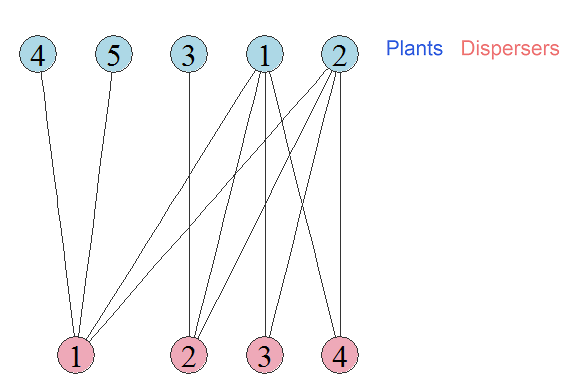
\includegraphics[scale=0.33]{Figures/VIS_SD_030_bipartita.png}
\caption{Diagrama bipartito de la red de dispersores de semillas que se usó como ejemplo de cálculo de las \textit{k magnitudes}. Véase la figura \ref{fig:ESTATICA_red_example}.}
\label{fig:Figures/VIS_SD_030_bipartita}
\end{figure}

En el ejemplo de la figura \ref{fig:Figures/VIS_SD_030_bipartita} puede distinguirse el núcleo de especies más conectadas (especies de plantas $1$ y $2$ y todos los polinizadores) y como las especialistas se conectan a él. Los enlaces se ven con claridad. No obstante, es difícil captar la estructura interna de la red como en la representación que utilizamos en la figura \ref{fig:ESTATICA_red_example}. El diagrama bipartito es ideal para redes de afiliación, en las que el dato clave es la conexión entre los nodos de ambas clases, pero no permite apreciar las interacciones indirectas entre elementos de una misma clase que comparten enlace con un nodo de la contraria.

\begin{figure}[h!]
\centering
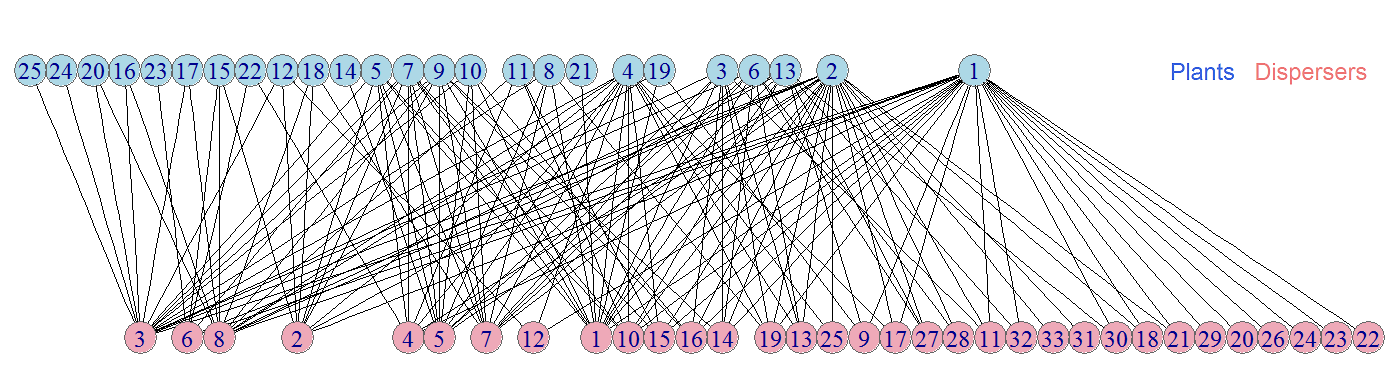
\includegraphics[scale=0.4]{Figures/VIS_bipartito_SD_020.png}
\caption{Red de dispersores en Nava Correhuelas, Sierra de Cazorla, España. Compilada por Pedro Jordano, no publicada.}
\label{fig:VIS_bipartito_SD_020}
\end{figure}

Cuando el número de especies supera unas pocas decenas, el diagrama bipartito se vuelve confuso. La red de la figura \ref{fig:VIS_bipartito_SD_020} tiene $58$ especies y $150$ enlaces, frente a $9$ especies y $11$ enlaces de la anterior. Es una red de dimensiones moderadas, pero es muy complicado seguir los detalles del gráfico. A pesar de ello, algunos autores consiguen resultados excelentes con redes de dimensiones similares a las de este segundo ejemplo, jugando con formas, colores y tamaños \cite{dakos2014critical}. Cuando se llega al centenar de especies, la zona central degenera en una mancha en la que es imposible distinguir los enlaces. Por este motivo, en la literatura sobre mutualismo no aparecen diagramas bipartitos de redes grandes. 

La matriz de adyacencia ofrece una visión más rica si los nodos se ordenan de la forma adecuada. Colocando los más conectados en la parte superior izquierda, es fácil localizar el núcleo de especies generalistas. Para redes pequeñas, el resultado es muy satisfactorio.

\begin{figure}[h!]
\centering
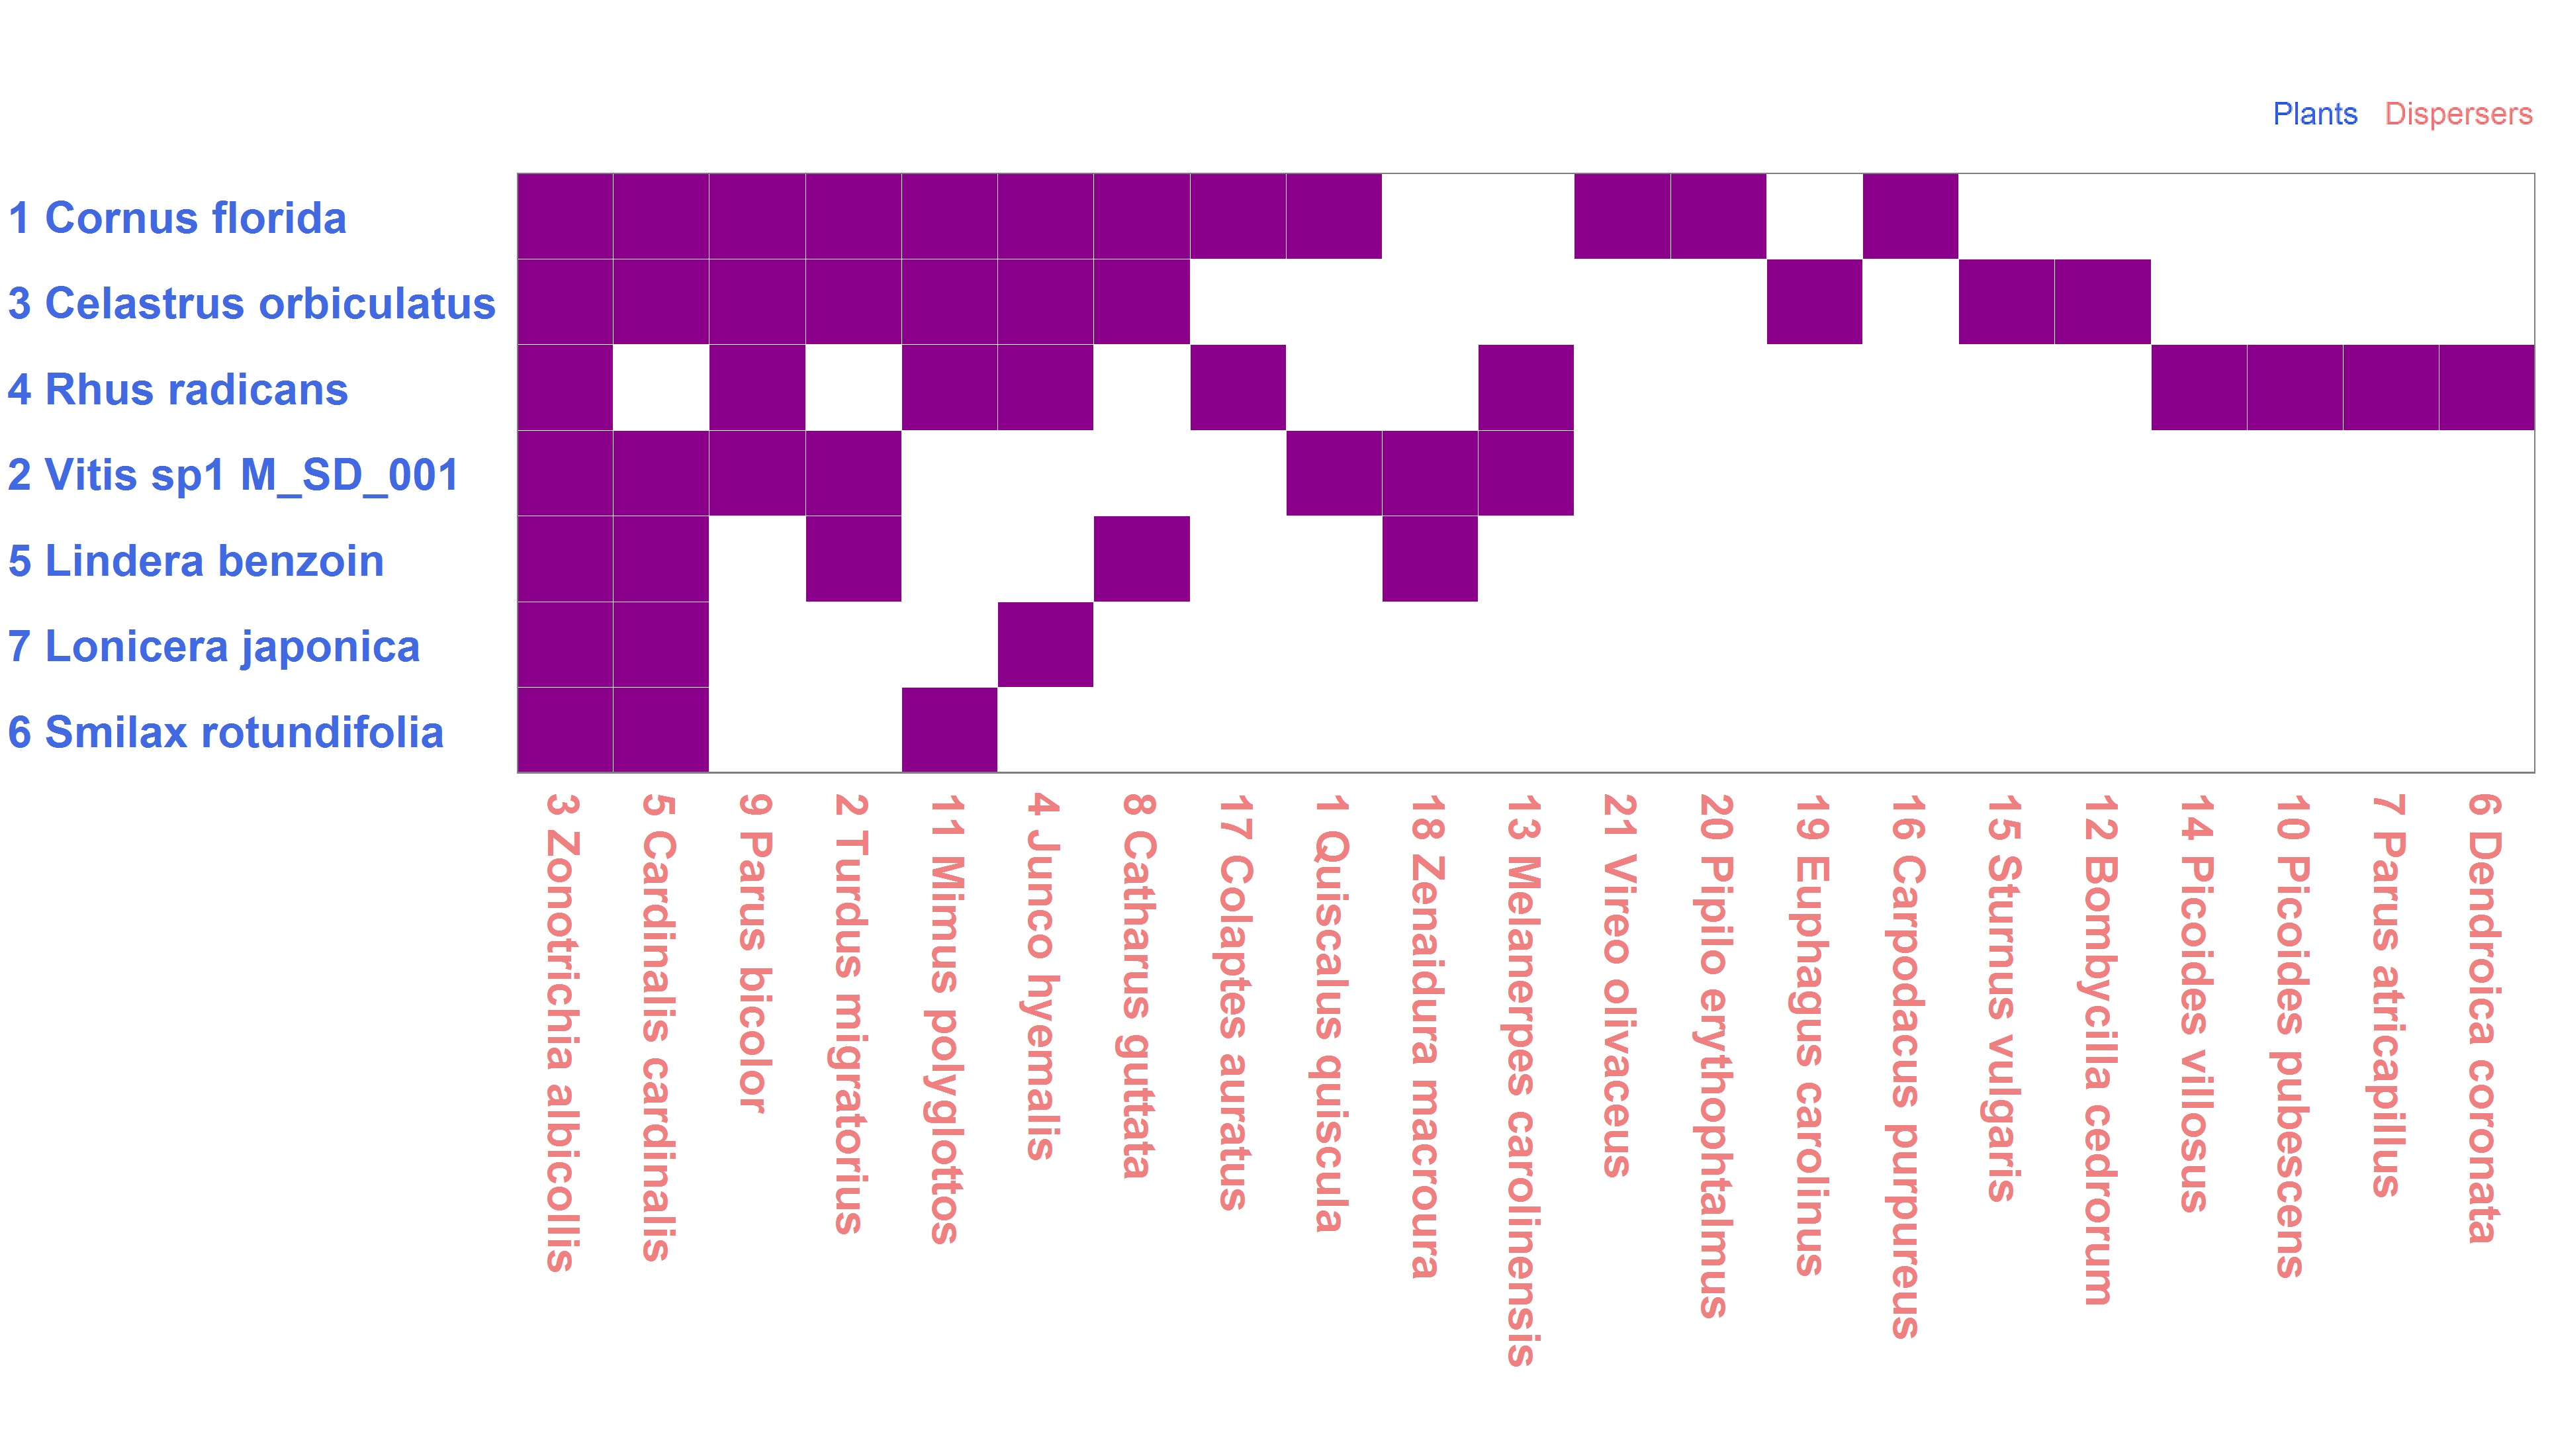
\includegraphics[scale=0.14]{Figures/VIS_matrix_SD_001.png}
\caption{Matriz de adyacencia de una red de dispersores en New Jersey \cite{baird1980selection}. Las casillas coloreadas indican la existencia de enlace.}
\label{fig:VIS_matrix_SD_001}
\end{figure}

Por el contrario, esta representación gráfica se vuelve también muy confusa para redes grandes, como muestra la figura \ref{fig:VIS_matrix_PL_001}.

\begin{figure}[hp!]
\centering
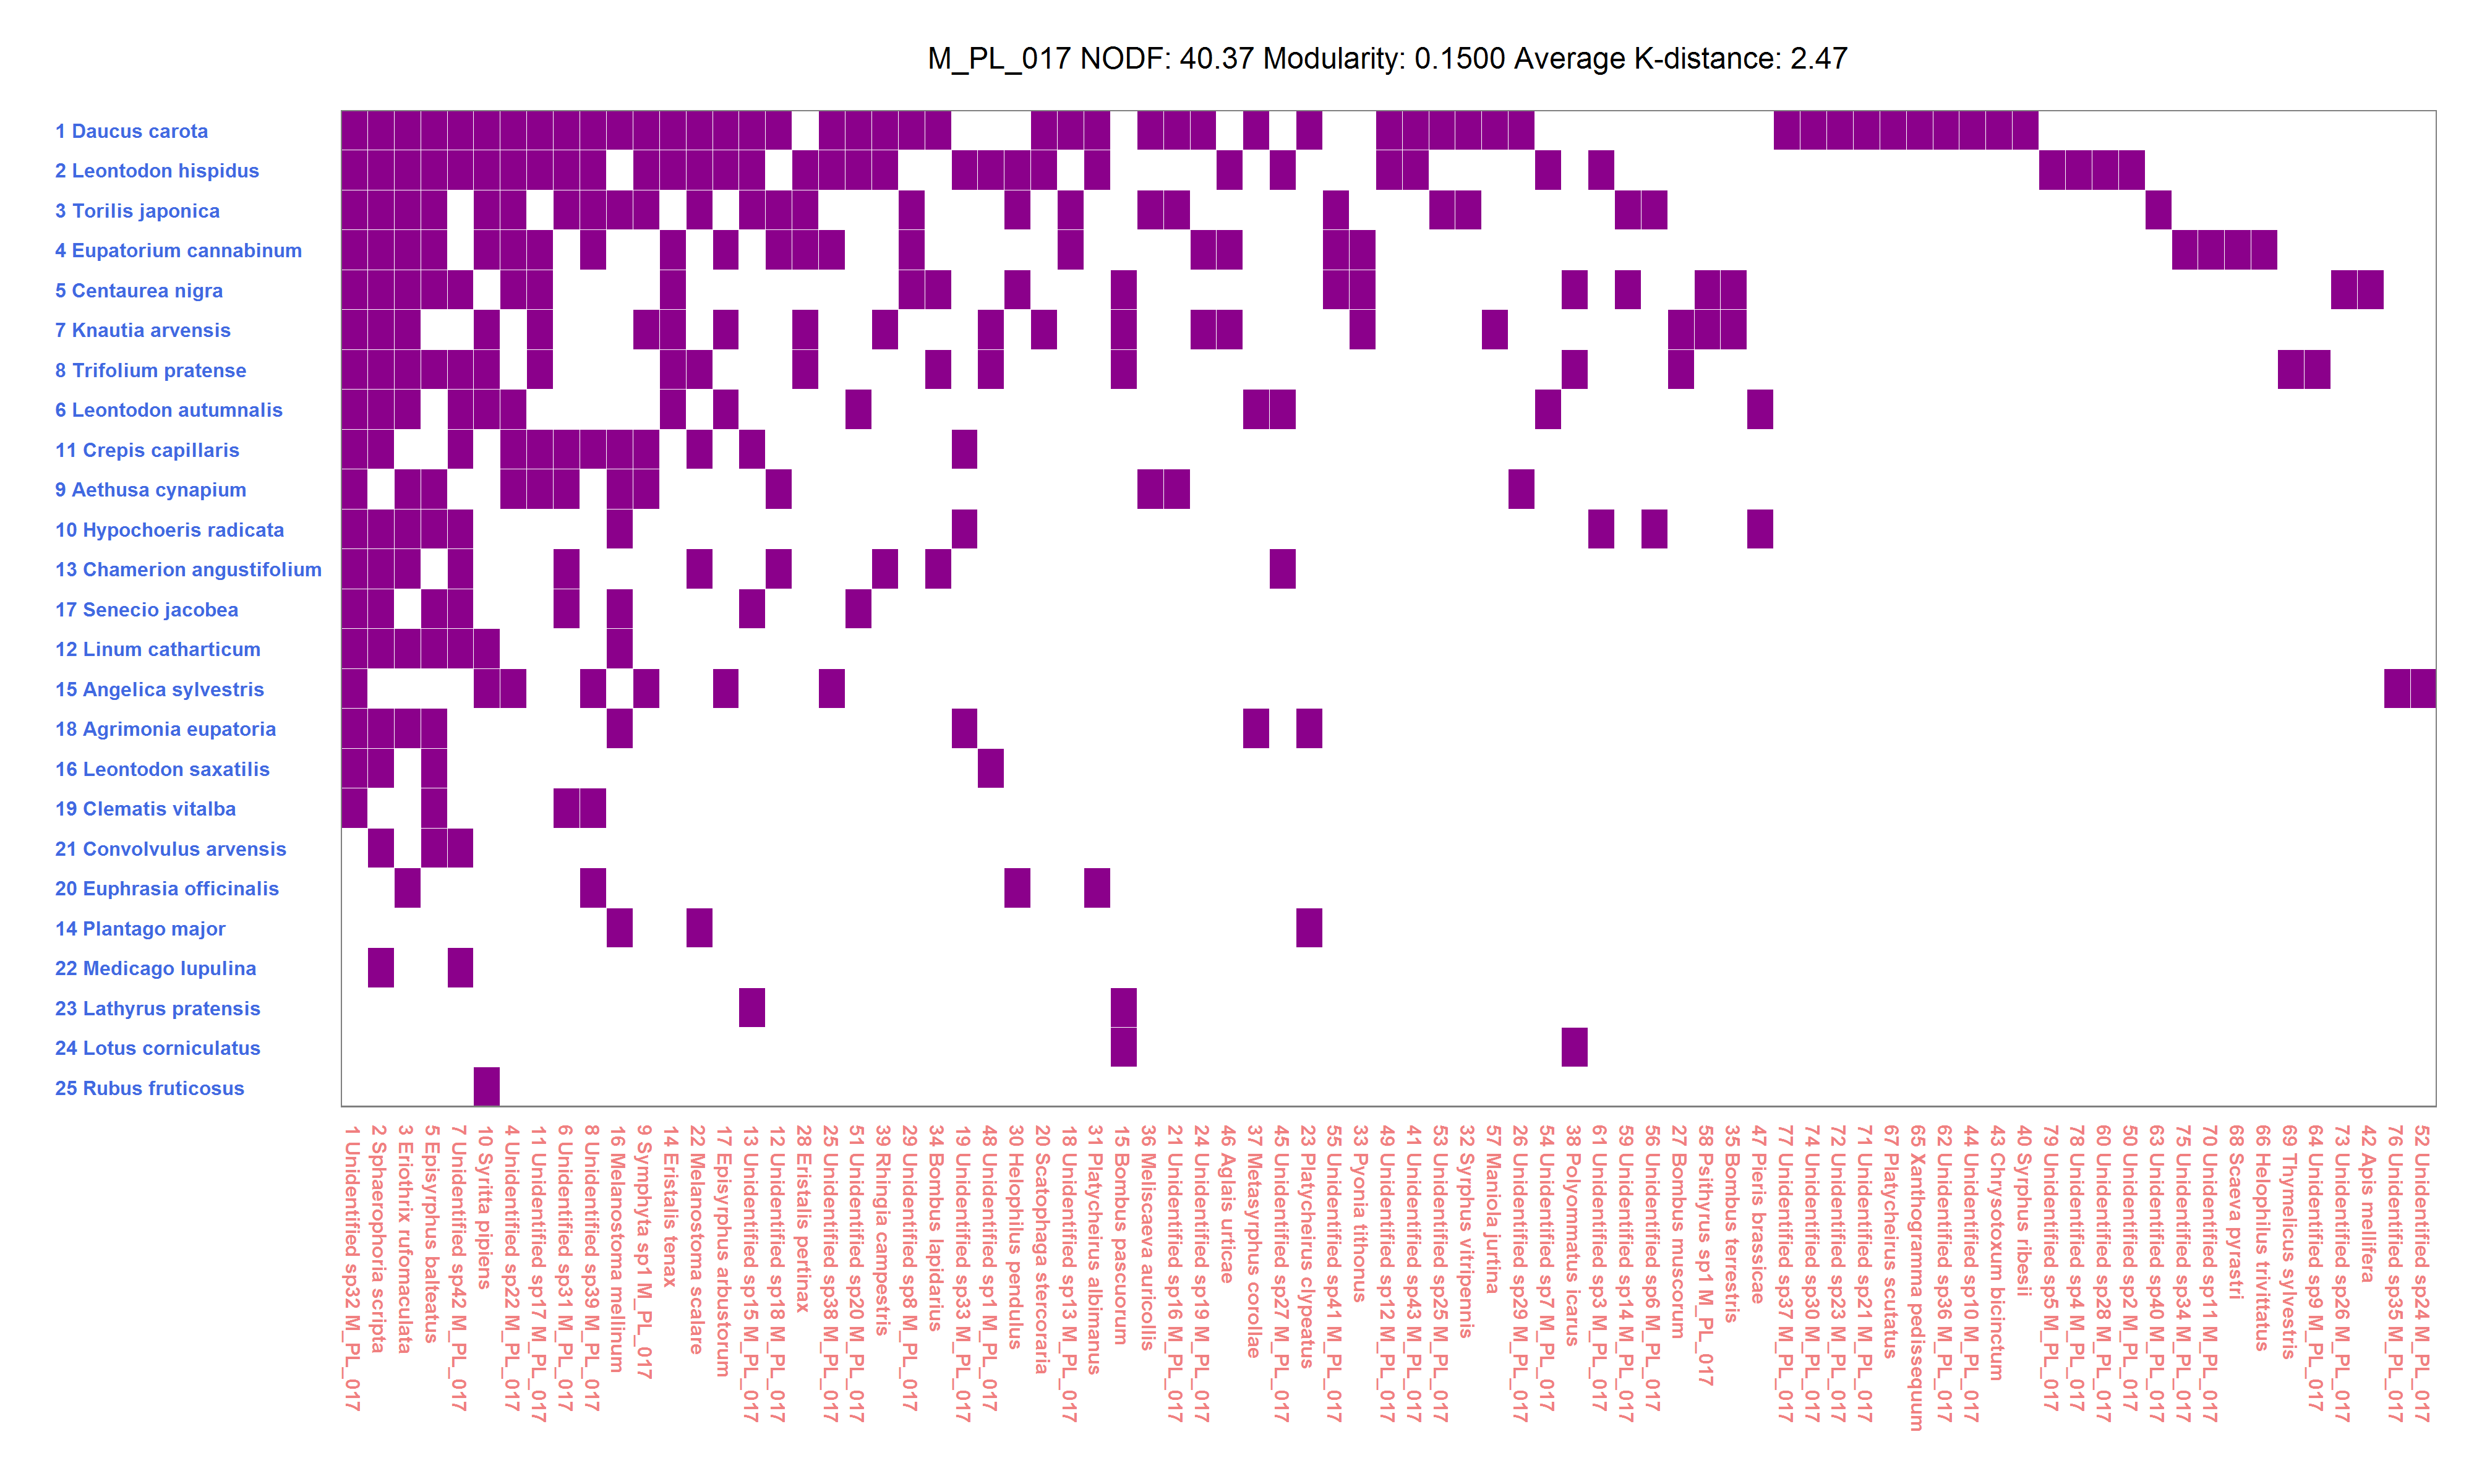
\includegraphics[scale=0.45]{Figures/VIS_M_PL_017_matrix.png}
\caption{Matriz de adyacencia de una red de polinizadores en Bristol, Inglaterra \cite{memmott1999structure}.}
\label{fig:VIS_matrix_PL_001}
\end{figure}

Una alternativa que algunos autores han explorado es utilizar representaciones convencionales para redes no bipartitas, asignando un color o forma específicos para cada clase \cite{mello2011missing,genini2010cheaters,toju2014assembly}. Esta solución tiene la ventaja de que se percibe mucho mejor la red y las relaciones indirectas que hemos mencionado. El precio que se paga es que los diagramas se vuelven muy complicados de entender con redes de tamaño medio (figura \ref{fig:VIS_grafos_weboflife}).

\begin{figure}[hp!]
\centering
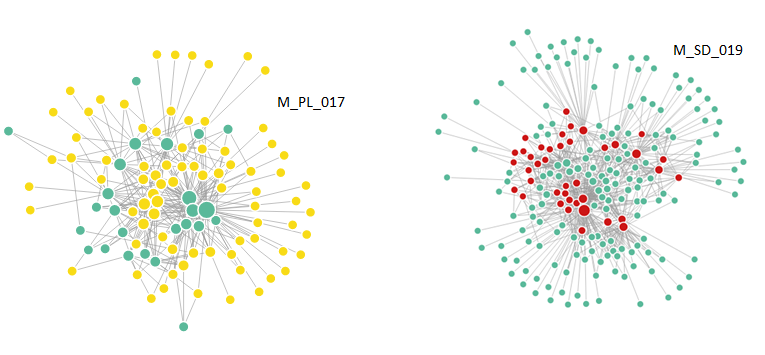
\includegraphics[scale=0.75]{Figures/VIS_grafos_weboflife.png}
\caption{Representación de dos redes de la colección \textit{web of  life} mediante la herramienta de visualización que ofrece la página web.}
\label{fig:VIS_grafos_weboflife}
\end{figure}

Estas limitaciones nos han llevado a diseñar visualizaciones específicamente adaptadas a las características de las redes mutualistas: bipartitas, con una fuerte jerarquía y en el rango de centenares de enlaces. 

\clearpage
\section{Visualizaciones basadas en \textit{k-magnitudes}}

En esta sección se describen dos nuevos tipos de visualización que se basan en las \textit{k magnitudes} definidas en el capítulo anterior: el diagrama polar y el diagrama zigurat.

\subsection{El diagrama polar}

El diagrama polar se inspira en el \textit{fingerprint plot}, desarrollado por Álvarez-Hamelin \textit{et al} y que se basa en la descomposición \textit{k-core} \cite{alvarez2005k}. Los autores emplearon esta técnica para reducir la información y poder visualizar redes muy grandes con índice $k$ máximo del orden de varias decenas. Los nodos se ubican de manera concéntrica, a una distancia que depende de su \textit{k-shell} y de las de sus vecinos. El tamaño de los nodos es proporcional al logaritmo del grado y el color indica la \textit{shell} a la que pertenecen. No se dibujan todos los enlaces, solo un pequeño porcentaje elegido al azar.

\begin{figure}[h!]
\centering
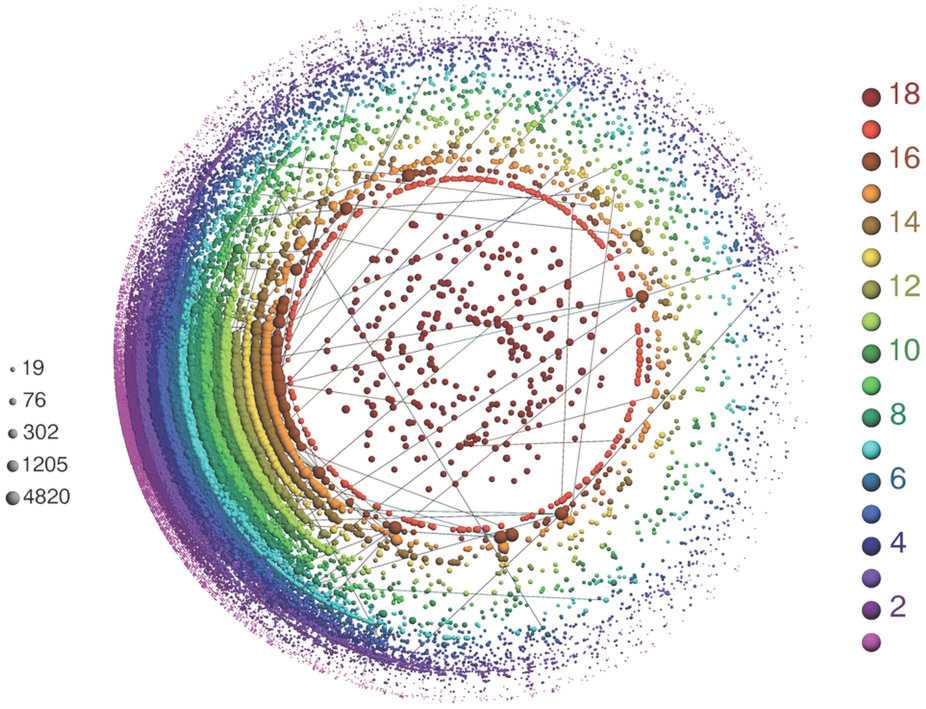
\includegraphics[scale=0.5]{Figures/VIS_fingerprint_plot.png}
\caption{\textit{Fingerprint plot} de la difusión de la noticia del descubrimiento del bosón de Higgs en Twitter \cite{de2013anatomy}. La imagen se generó con el software \texttt{LaNet-vi}, desarrollado por el equipo que creó este tipo de diagrama \cite{alvarez2008low}.}
\label{fig:VIS_M_PL_034_polar}
\end{figure}

Una versión evolucionada de esta forma de representar redes grandes usando la descomposición \textit{k-core} utiliza las \textit{k-shell} en lugar de los nodos. Estas se dibujan como círculos que se disponen en espiral alrededor de la \textit{shell} máxima (figura \ref{fig:VIS_taksim}).

\begin{figure}[h!]
\centering
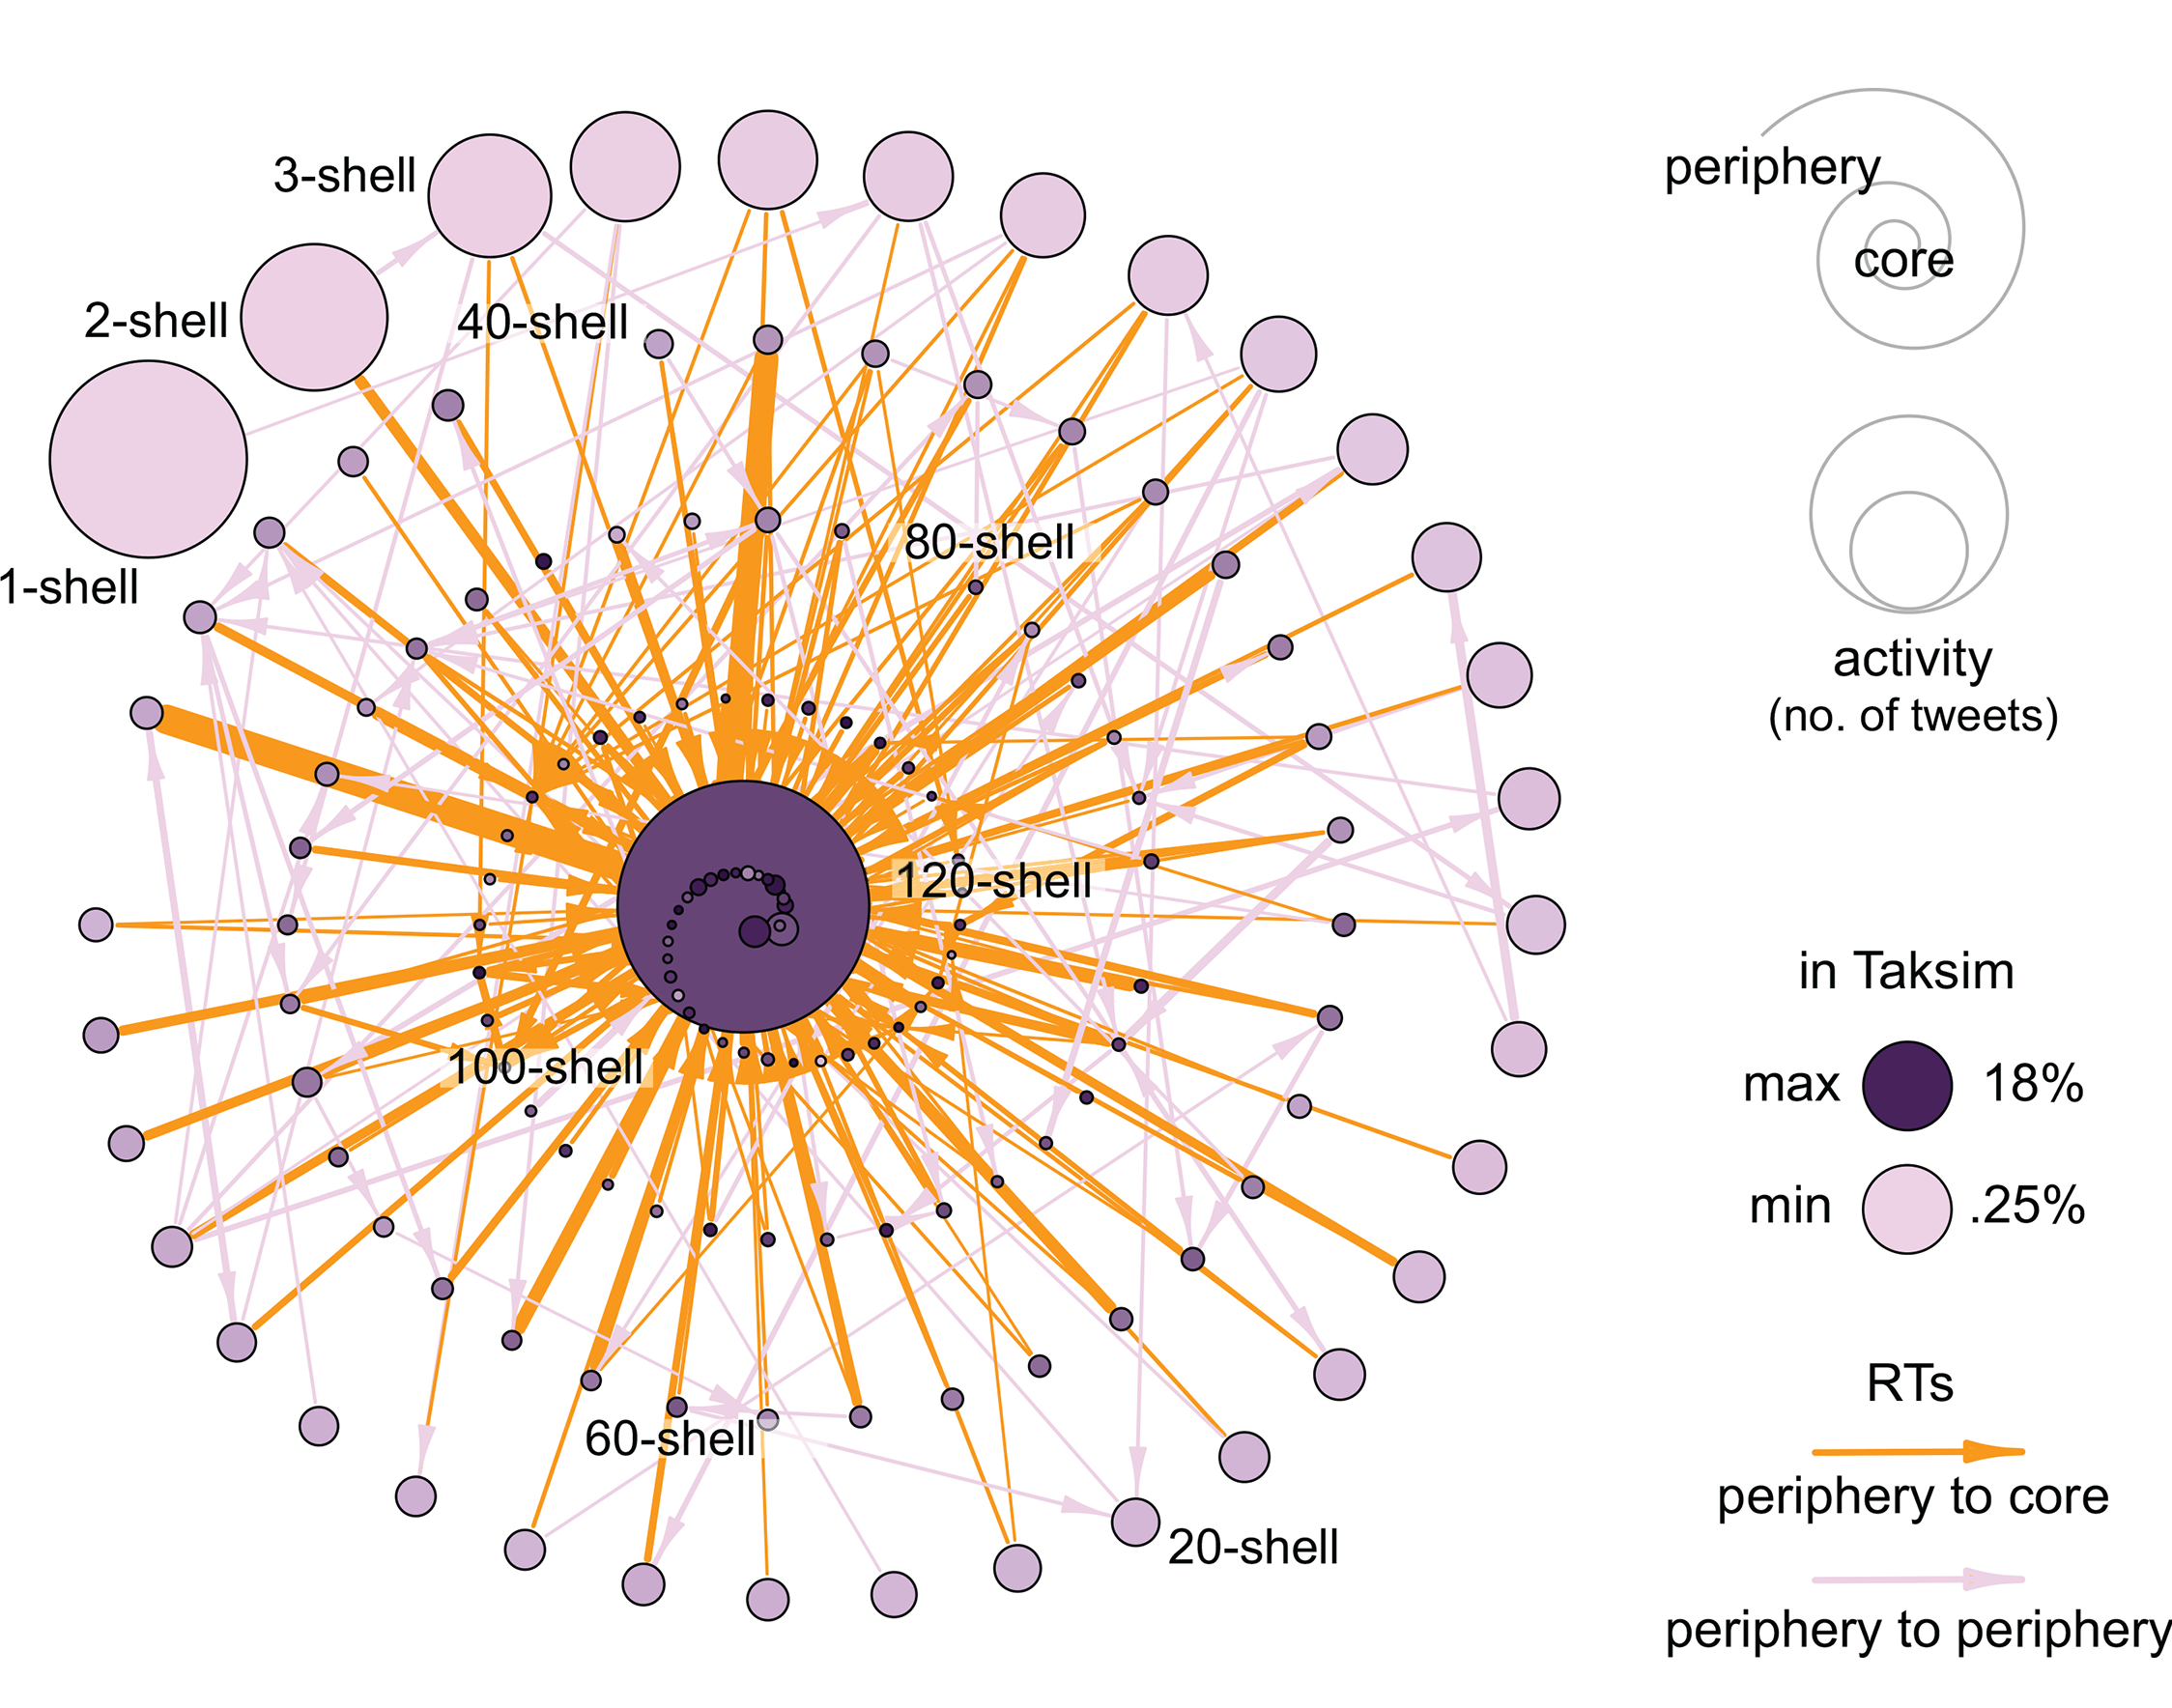
\includegraphics[scale=0.6]{Figures/VIS_taksim.png}
\caption{Diagrama de relaciones entre las \textit{k shells} de retweets de los participantes en las protestas del parque Taksim Gezi en Estamnul en 2013   \cite{barbera2015critical}.}
\label{fig:VIS_taksim}
\end{figure}


En el \textit{diagrama polar} se conservan las ideas de diagrama concéntrico y la coloración en función del \textit{k-shell}, pero hay cambios profundos en el resto de detalle. La naturaleza bipartita de las redes mutualistas es la principal diferencia con el \textit{fingerprint plot} original. En el diagrama polar cada clase ocupa uno de los semiplanos, divididos horizontalmente. La forma de los nodos se emplea para remarcar esta diferencia. 

El centro de cada especie se sitúa a una distancia $k_{radius}$ del origen de coordenadas. Recordemos que el valor mínimo de esta magnitud es $1$. El tamaño de los nodos es proporcional a su $k_{degree}$ y el color propio de la \textit{k-shell}. El algoritmo de representación asigna el ángulo que se distribuye para evitar al máximo la superposición de nodos. Una diferencia sustancial con el  \textit{fingerprint plot} es que en este tipo de visualizació no se representan los enlaces.

\begin{figure}[h!]
\centering
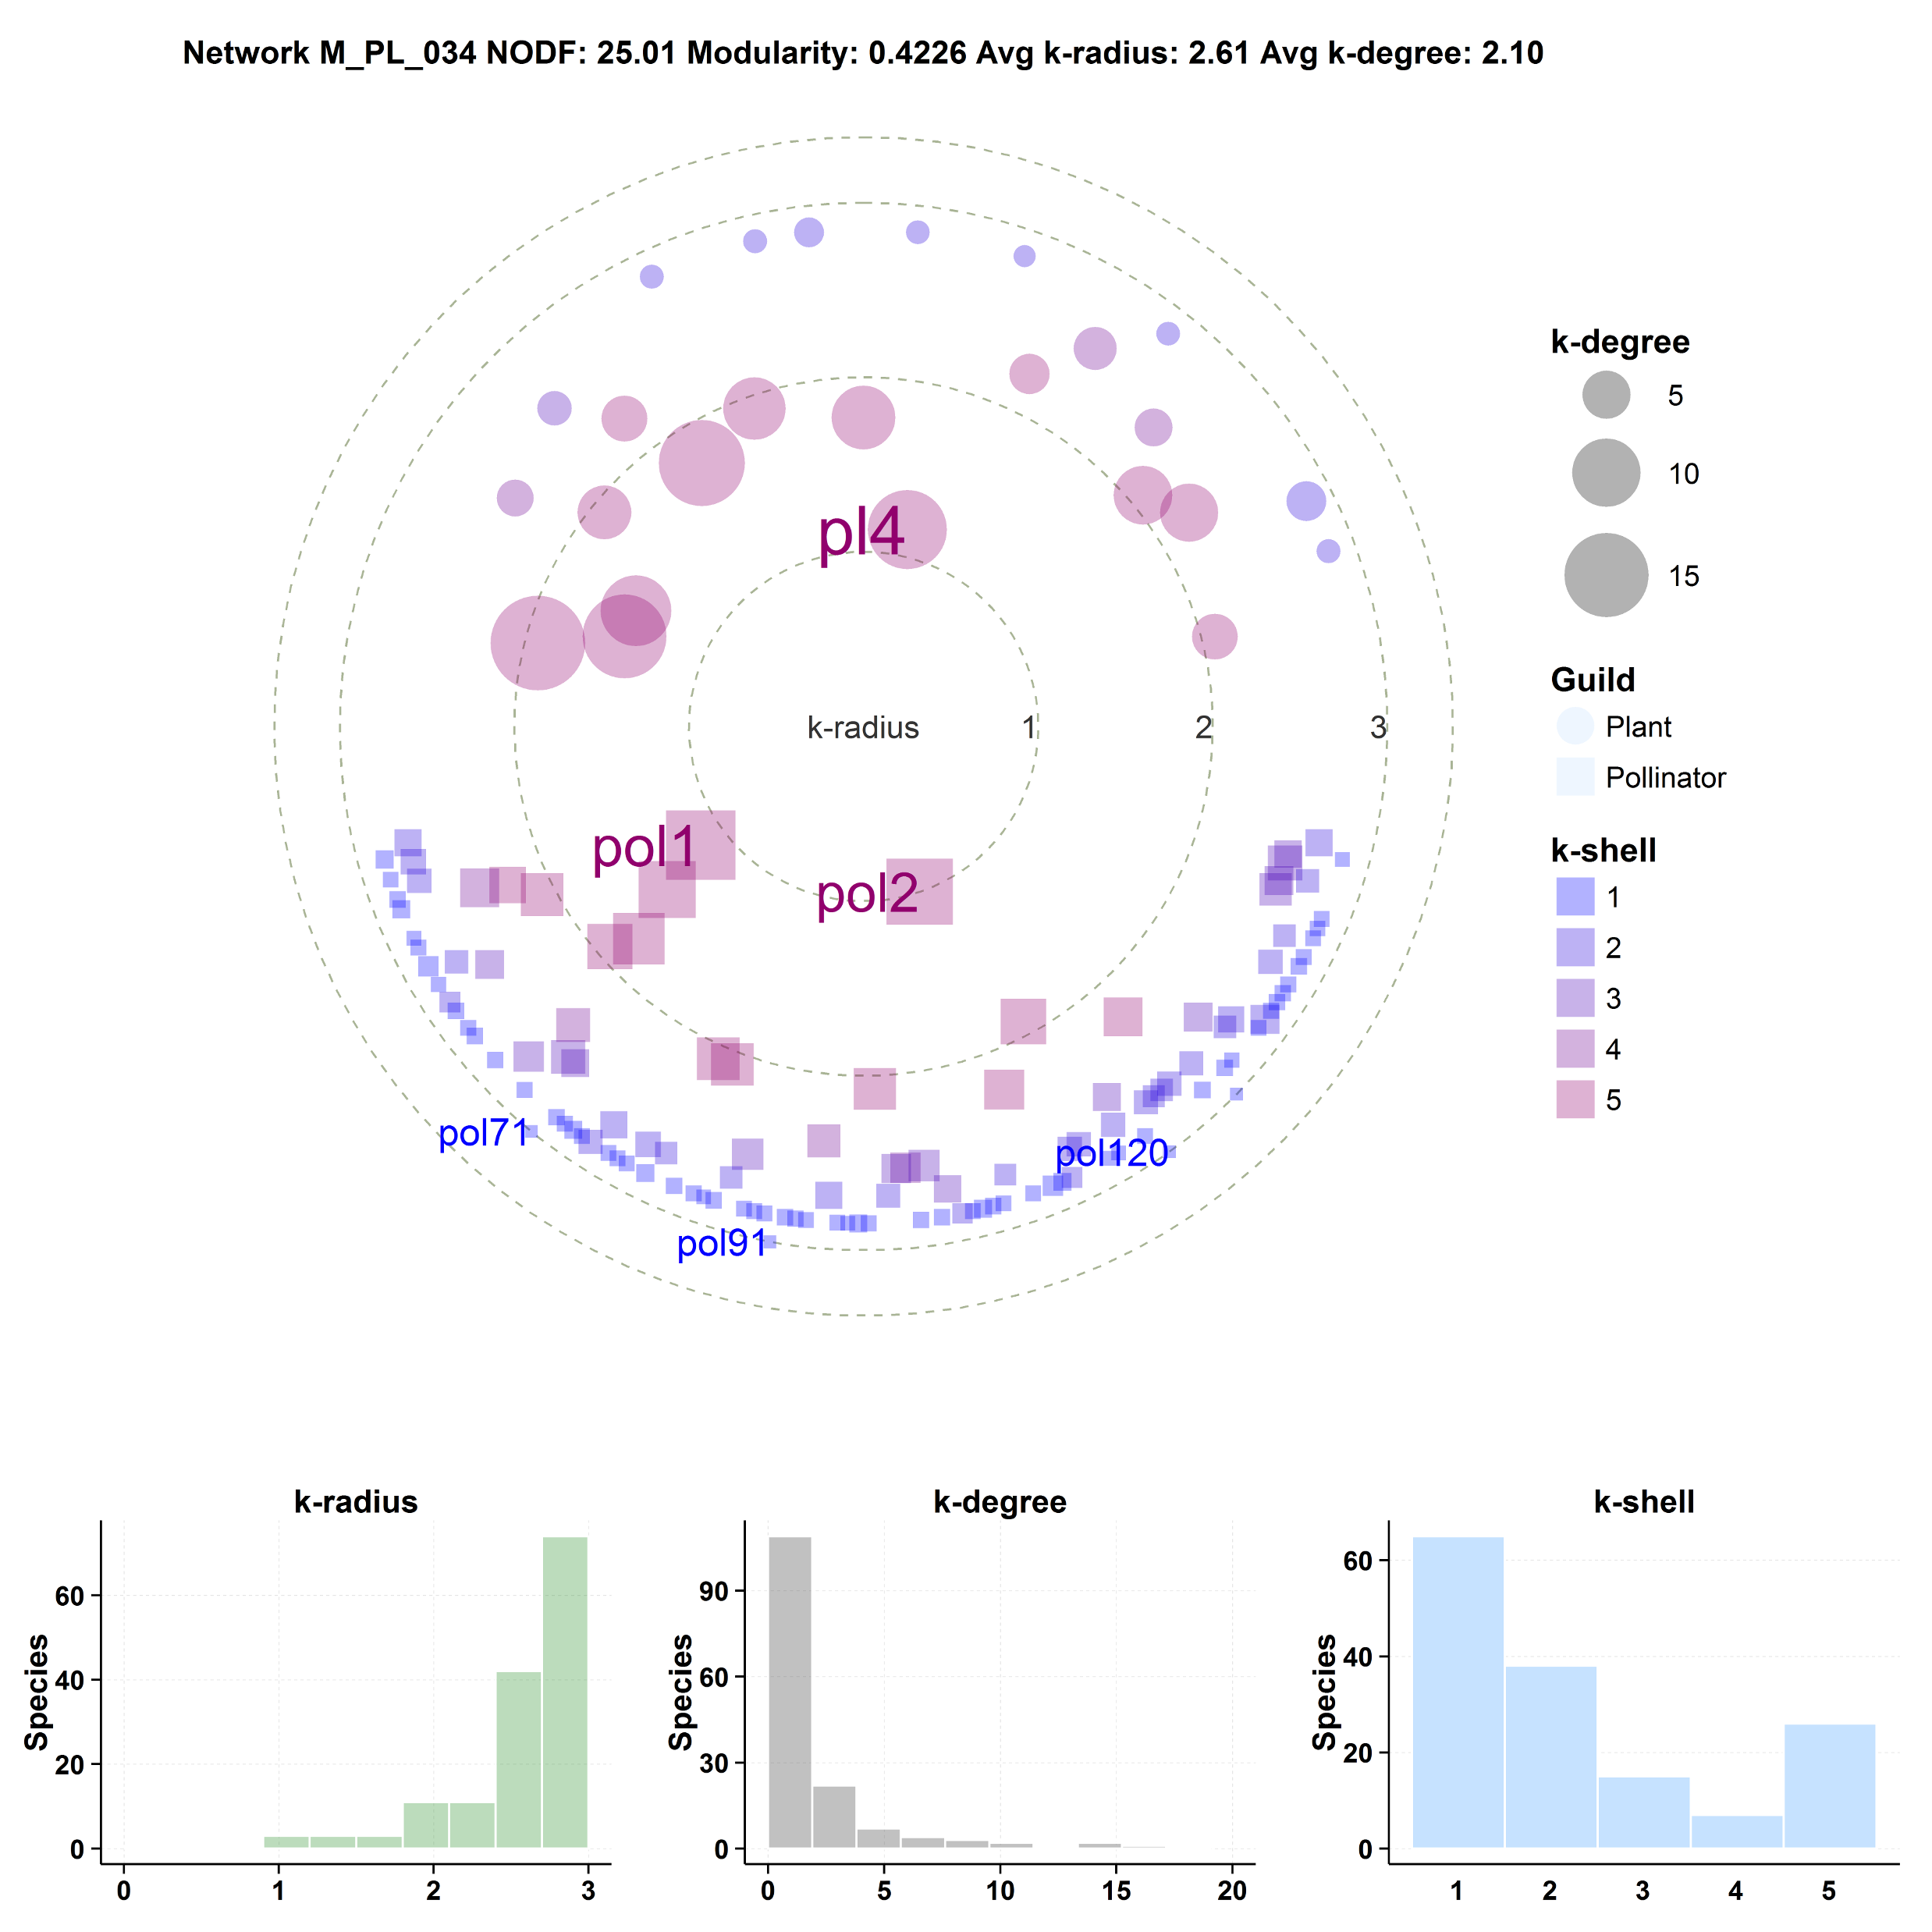
\includegraphics[scale=0.4]{Figures/VIS_M_PL_034_polar.png}
\caption[PolarExample]{Diagrama polar de una comunidad de polinizadores en la isla de Chiloé (Chile) \cite{smith2005diversity}.}
\label{fig:VIS_M_PL_034_polar}
\end{figure}

Se puede elegir incluir los nombres de todas las especies, de ninguna, o de un pequeño número, por defecto las tres más centrales y las tres más alejadas. Además, el usuario puede decidir que se añadan los histogramas de las tres \textit{k-magnitudes}, que contienen información muy valiosa.

La figura \ref{fig:VIS_M_PL_034_polar} es la representación polar de una red de polinizadores, que hemos elegido por ser una red mutualista tipo tanto por tamaño, anidamiento, modularidad y valores de las \textit{k magnitudes}, todos ellos no demasiado alejados de la media (tabla \ref{table:table_results}). El histograma de la distribución por \textit{k shells} tiene forma de bañera, muy repetido en estas redes. Hay unos pocos nodos dominantes y centrales, de índice $k = 5$ y un número importante de especies en las \textit{shells} exteriores. Es una red de elevada asimetría de especies ($0.66$), véase tabla \ref{table:table_results_recableados}).

La utilidad del diagrama polar se descubre al comparar varias redes, incluso si son de tamaños muy dispares. En la figura \ref{fig:VIS_Modvskdegree3}, se han escogido tres redes situadas en ambos extremos y en el centro del diagrama \ref{fig:ESTATICA_corrfigs} (derecha). La red de polinizadores $PL\_010$  tiene un valor de $Modularity$ bajo $(0.25)$, y alto el de $\overline {k}_{degree}$ $(4.57)$. El diagrama polar muestra la estructura en capas del mutualismo. Esta es mucho más evidente en la red $SD\_007$ ($Modularity: 0.28$, $\overline {k}_{degree}: 2.34$). La distribución de $\overline {k}_{degree}$ es más abrupta, con dos especies muy dominantes. La imagen transmite la idea de que esta red tiene una mayor organización jerárquica que $PL\_010$.

La red $PL\_021$ es grande y fuertemente modular ($Modularity: 0.57$, $\overline {k}_{degree}: 1.23$). La distribución de $\overline {k}_{degree}$ es aun más abrupta. Se ha incluido en la parte inferior izquierda la distribución de densidades que ya aparecía en la figura \ref{fig:ESTATICA_density_plots} porque la escala logarítmica en el eje horizontal permite ver mejor las diferencias.

\begin{figure}[h!]
\centering
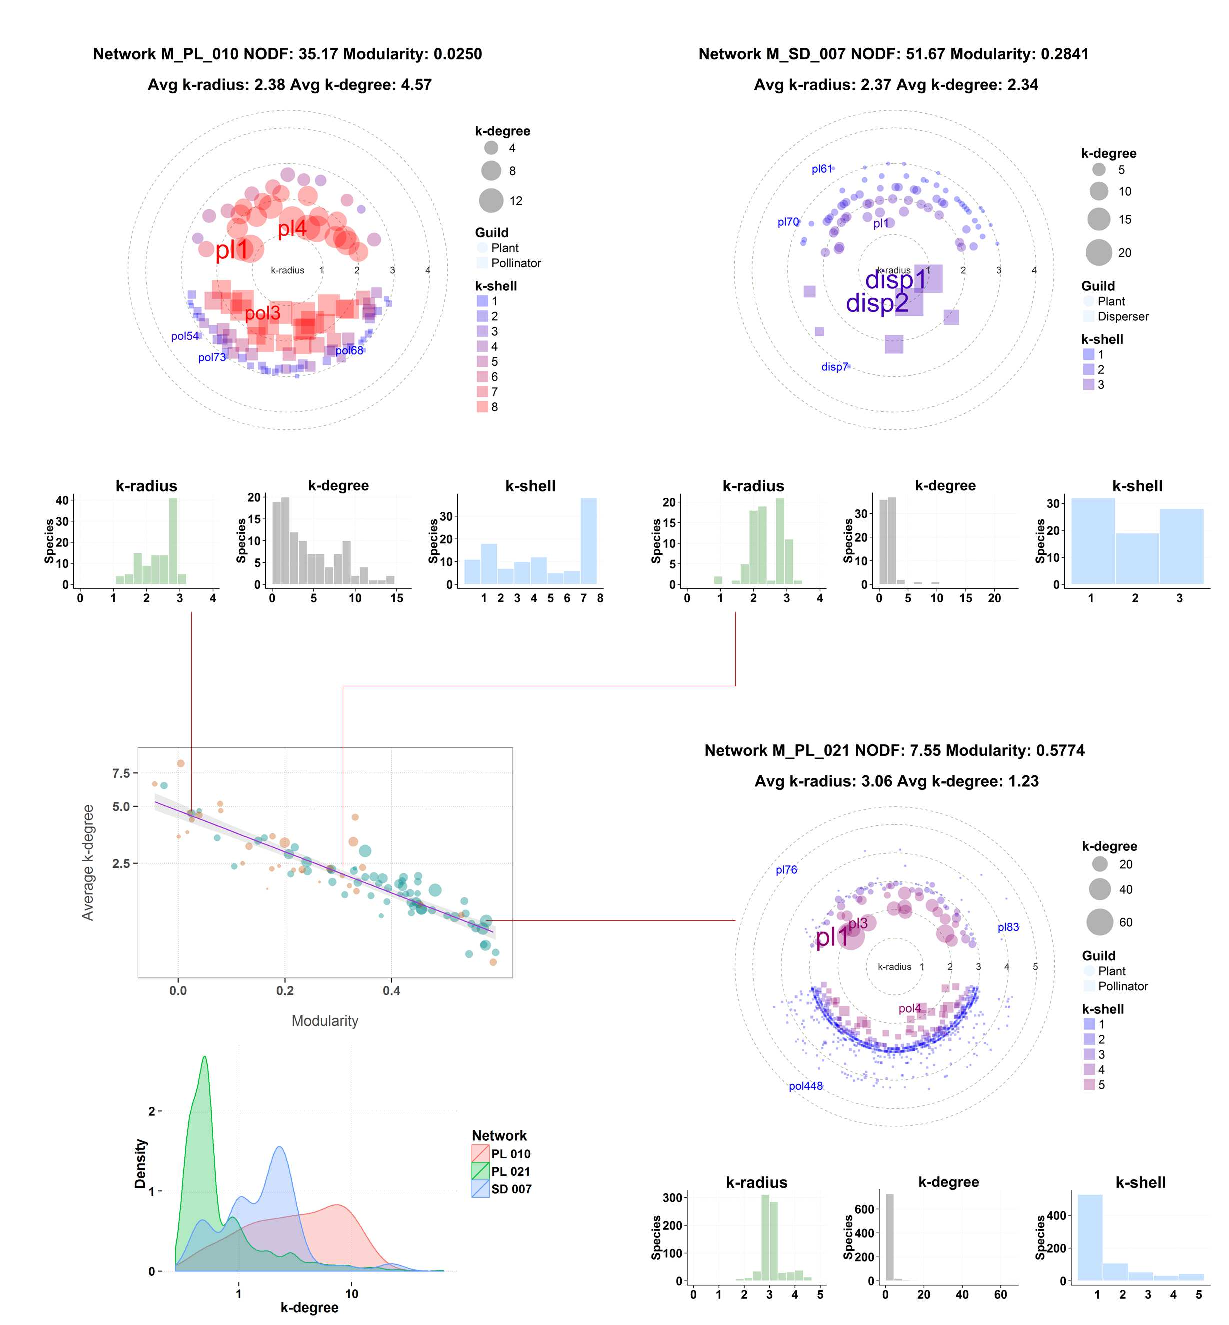
\includegraphics[scale=0.75]{Figures/VIS_Modvskdegree3.PDF}
\caption[PolarExample]{Comparación de tres redes mediante sus diagramas polares.}
\label{fig:VIS_Modvskdegree3}
\end{figure}

A pesar de que el diagrama polar ofrece una nueva visión de las comunidades mutualistas, tiene limitaciones. Como en toda estrategia de reducción de la información hay que renunciar a representar detalles en favor de una mejor visibilidad, en este caso los enlaces. No se trata de un detalle menor, así que se ha desarrollado un segundo tipo de diagrama que los toma como base de su construcción.

\clearpage
\subsection{El diagrama zigurat}
\label{sec:diagrama_zigurat}

El diagrama zigurat se ha creado para mostrar la estructura de \textit{k shells} de una red bipartita y los enlaces entre sus nodos. La idea básica consiste en agrupar las especies en \textit{shells} que se representan como pequeños zigurats\footnote{Según el DRAE: Torre escalonada y piramidal, característica de la arquitectura religiosa asiria y caldea.}. Las dos \textit{shells} máximas se colocan en el eje de simetría horizontal, ligeramente hacia la izquierda. El resto, se distribuyen siguiendo una disposición en forma de almendra, que deja un gran espacio libre para dibujar los enlaces.

\begin{figure}[h!]
\centering
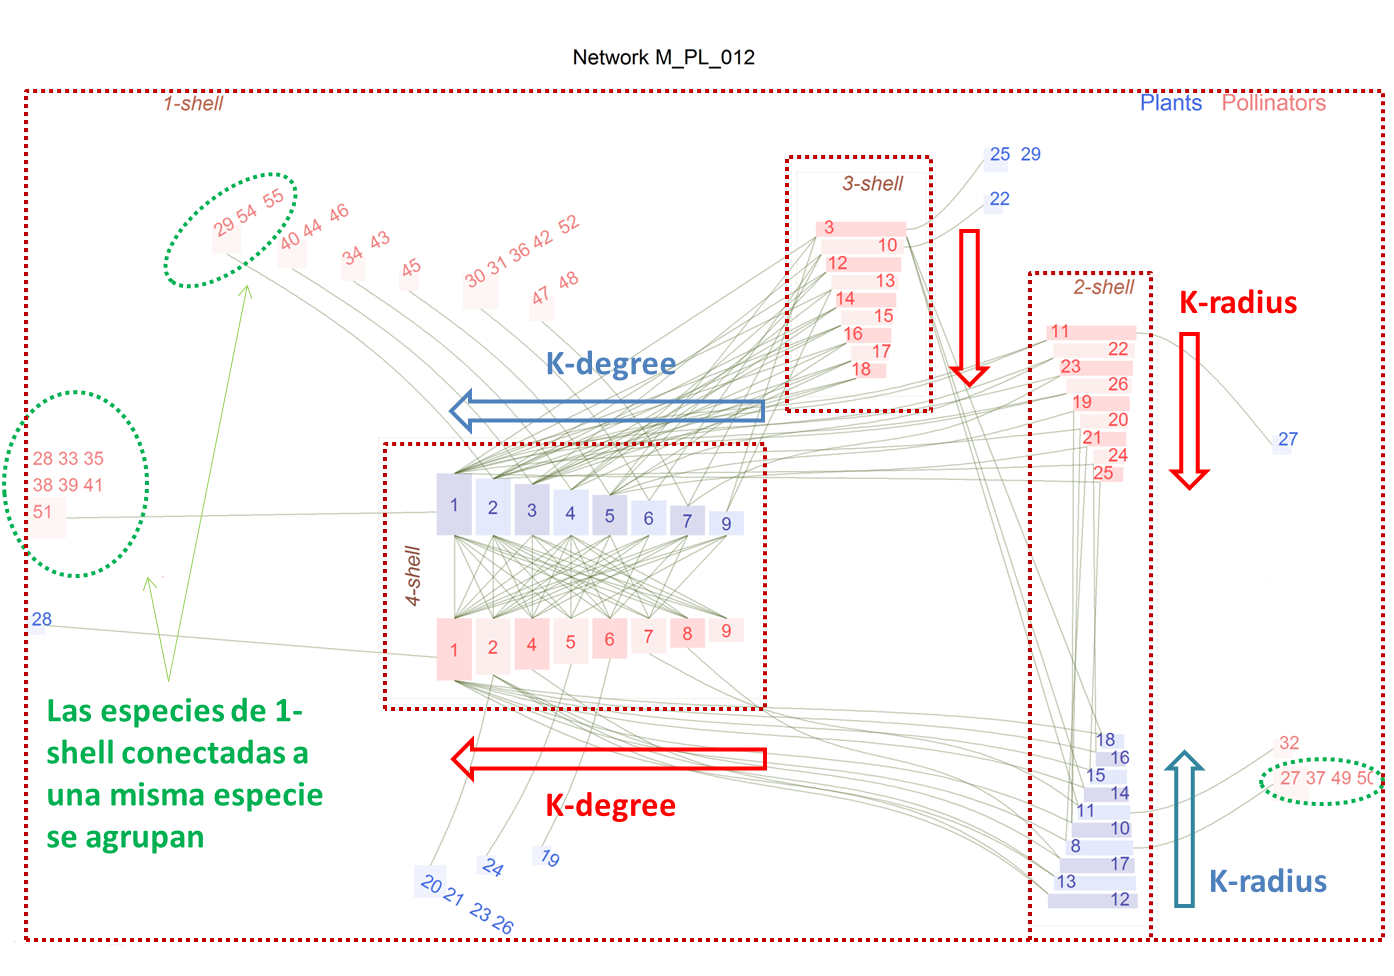
\includegraphics[scale=0.4]{Figures/VIS_explicacion_zigurat.png}
\caption {Estructura del diagrama zigurat para la red  $M\_PL\_012$.}
\label{fig:VIS_explicacion_zigurat}
\end{figure}

Las clases se diferencian por el color de relleno. Para cada una se emplean dos tonalidades del mismo color lo que facilita la lectura del diagrama. Las especies se indican por el número
con el que figuran en el fichero de datos, de $1$ a $m$ para una clase y de $1$ a $n$ para la otra.

En la \textit{shell} máxima las especies se ordenan por $k_{degree}$, con el valor mayor en el extremo izquierdo. Esta disposición facilita la colocación a su altura del grupo de especies de la $1$-$shell$ con las que se conecta, que pueden llegar a ser muy numerosas. En el resto de \textit{shell}, las especies se ordenan por $k_{radius}$, correspondiendo la base del zigurat a la de menor $k_{radius}$.

\begin{figure}[hb!]
\centering
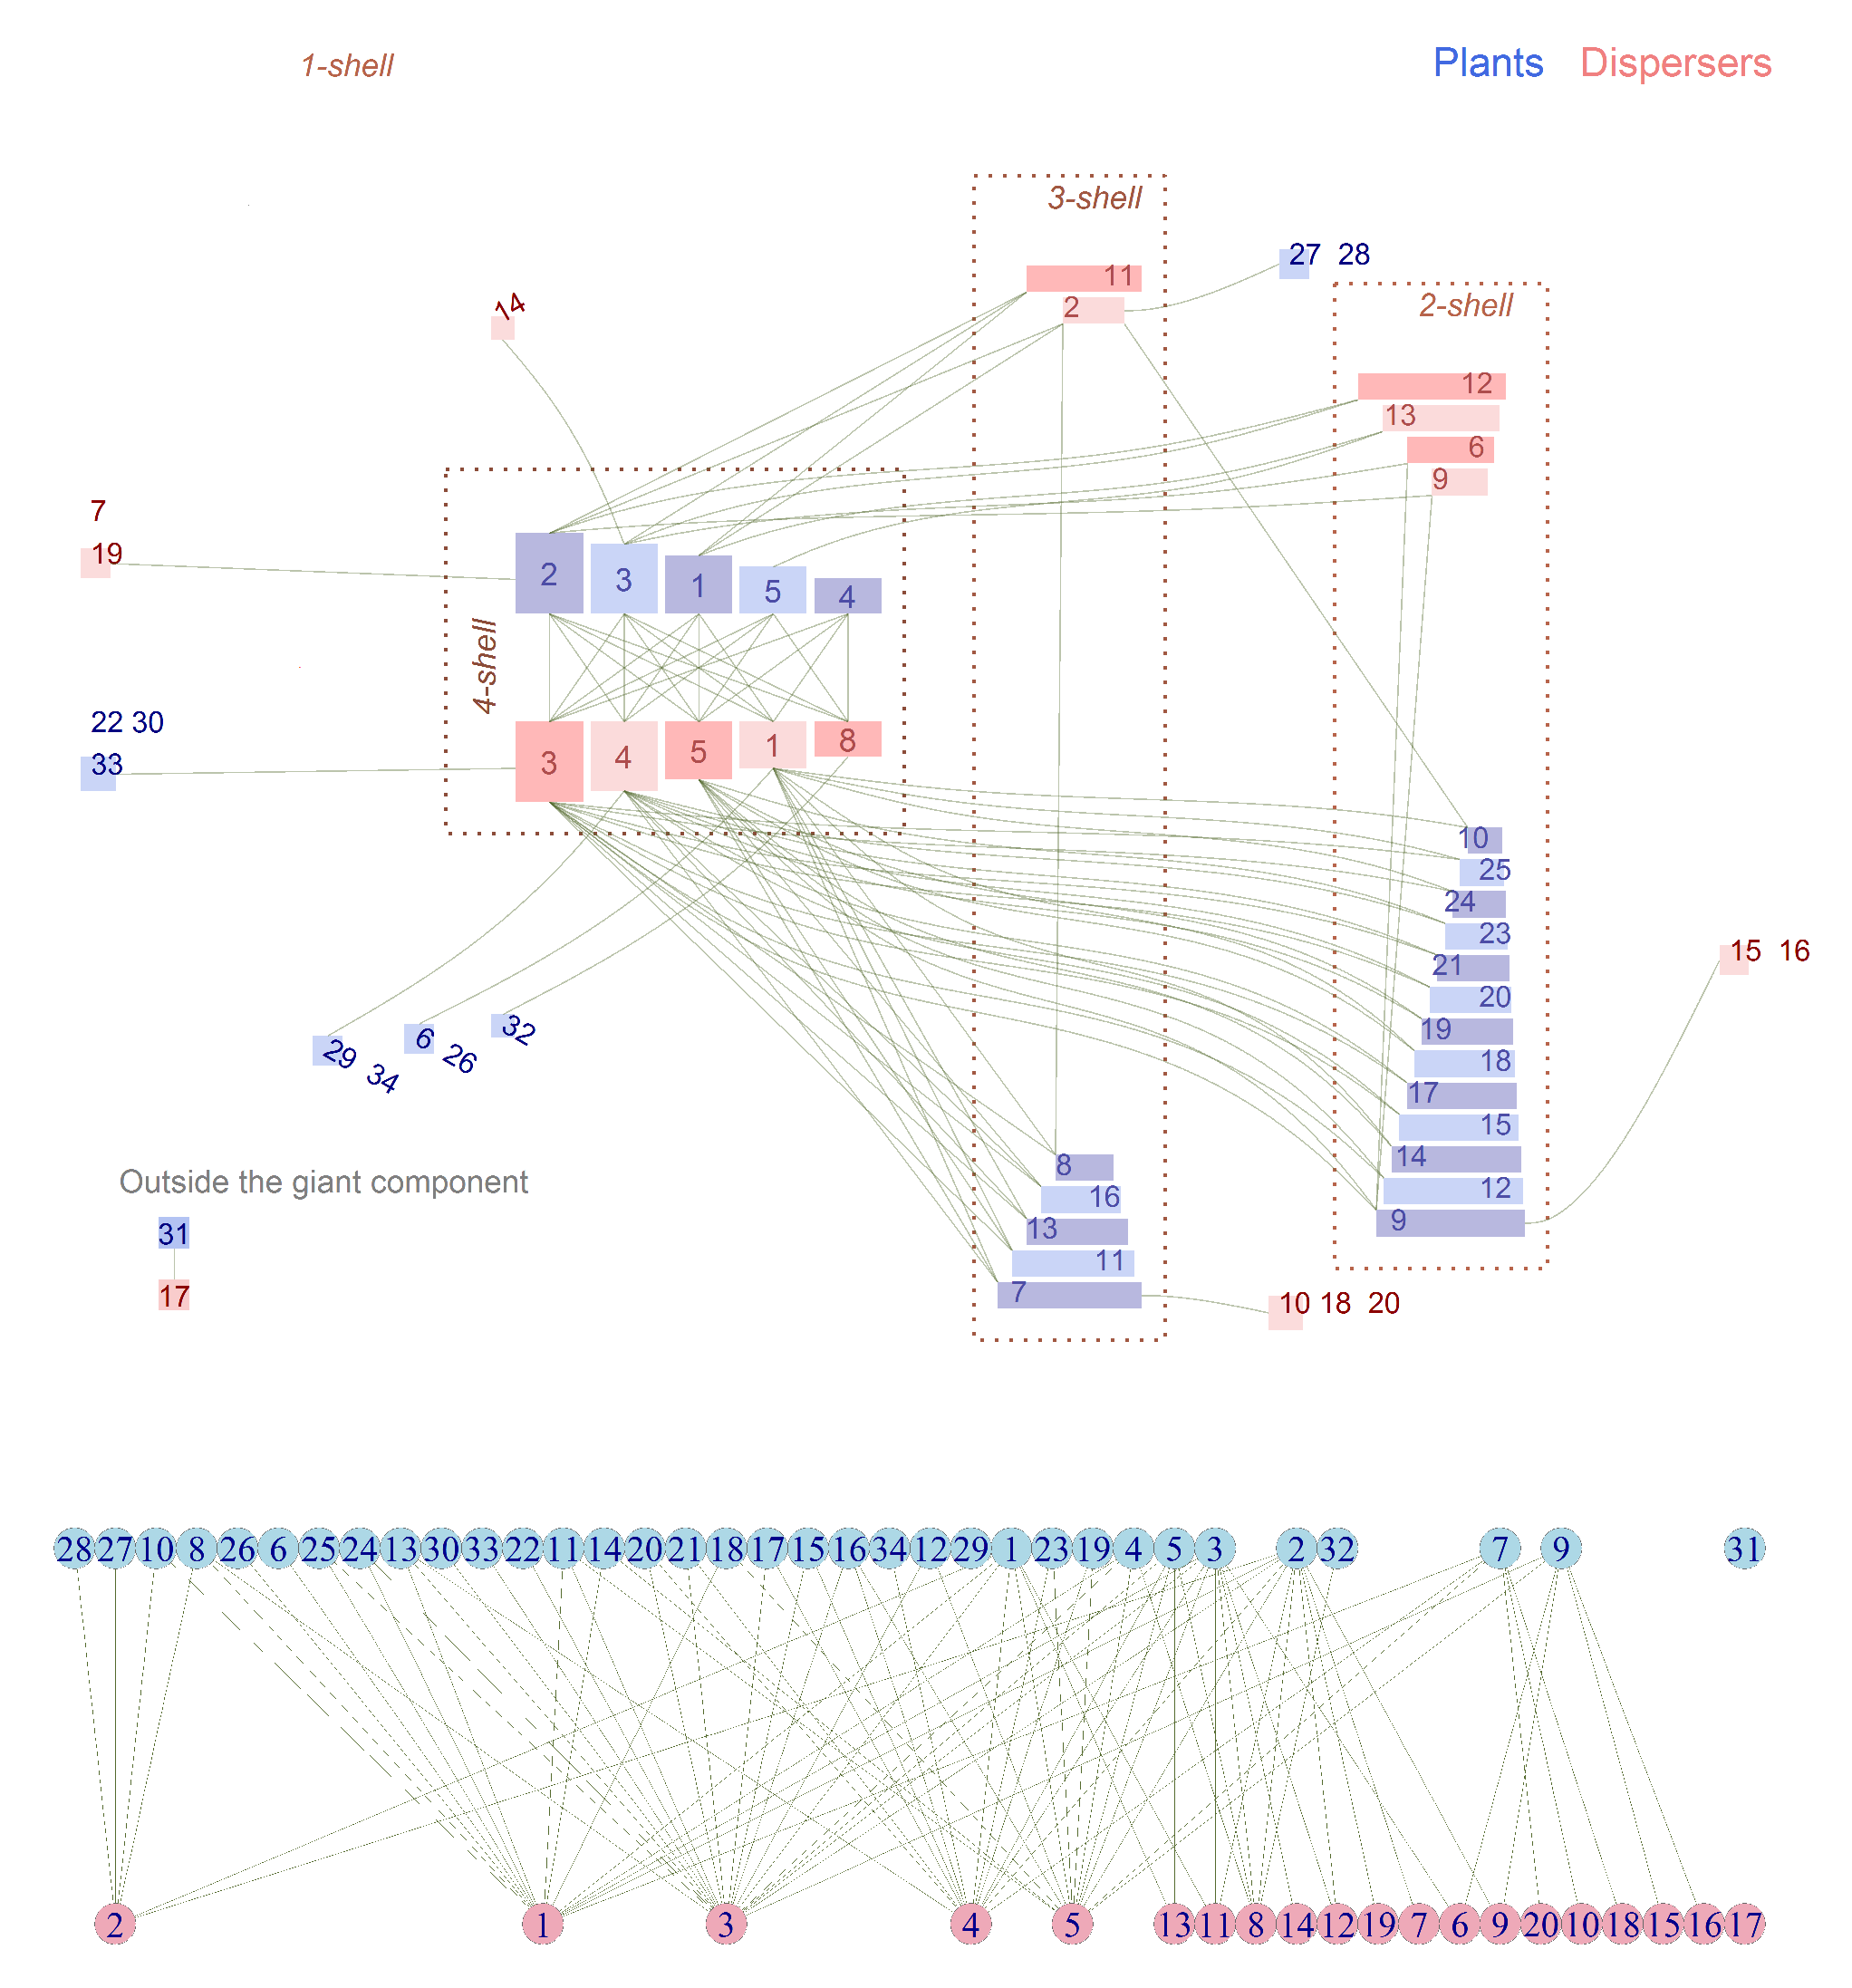
\includegraphics[scale=0.45]{Figures/VIS_ALL_SD_004.eps}
\caption {Diagrama zigurat de una comunidad de aves frugívoras de Puerto Rico  $M\_SD\_004$, con $54$ especies y $95$ enlaces \cite{carlo2003avian}. $\overline k_{radius} = 2,19$; $\overline k_{degree} = 2,37$; $NODF = 39,82$; $Modularity = 0.34$. Abajo el diagrama bipartito.}
\label{fig:ziggurat}
\end{figure}

Los enlaces entre especies de la \textit{shell} máxima se representan entre las bases de sus rectángulos. El enlace entre dos especies de \textit{shells} de distinto índice conecta el lado izquierdo de la de índice inferior y el derecho de la de la de índice superior, salvo que sea la máxima, en cuyo caso se usa el extremo superior. Los enlaces entre especies de la misma \textit{shell} conectan los extremos izquierdos de ambas.

Las especies de la $1$-$shell$ se disponen como una nube el torno a los zigurats de la almendra central. Si, como sucede a menudo, varias especies de esta \textit{shell} comparten la única especie con la que se conectan, se dibujan de forma agrupada y con un único enlace. Puede verse en los ejemplos dentro de las elipses punteadas en verde de la figura \ref{fig:VIS_explicacion_zigurat}. Pueden distinguirse las tres ubicaciones características de estos grupos: a la izquierda de la \textit{k shell} máxima (para los conectados a la especie de mayor $k_{degree}$), encima del resto de las especies de esta \textit{shell} y a la derecha de los demás zigurats.


En algunas redes se incluyen observaciones de especies que no están conectadas con la componente gigante. En ese caso, se representa el fragmento inconexo, pero no se tiene en cuenta para la \textit{k descomposición}.

Un detalle importante es que en el diagrama zigurat, las áreas no transmiten información. Se han dispuesto así por conveniencia para poder representar con la mayor claridad posible los enlaces y las agrupaciones en \textit{k shells}.

La red de la figura \ref{fig:ziggurat} es de pequeño tamaño y produce una figura que recuerda a un pez con su boca y aletas. Esta imagen se repite en numerosos ejemplos. En el gráfico bipartito todavía se pueden seguir los enlaces individuales. Sin embargo, el zigurat ofrece una visión mucho más rica de la organización con cuatro \textit{shells} internas y la $1$-$shell$ con pocas especies. Se pueden descubrir con facilidad algunos patrones, como la baja conectividad entre especies de las \textit{shells} de menor índice $k$, o la relativa importancia de la especie dispersora $2$ que en el bipartito aparece en el extremo izquierdo. Hay dos especies desconectadas de la componente gigante, pueden verse en la parte inferior izquierda del diagrama.

\begin{figure}[hp!]
\centering
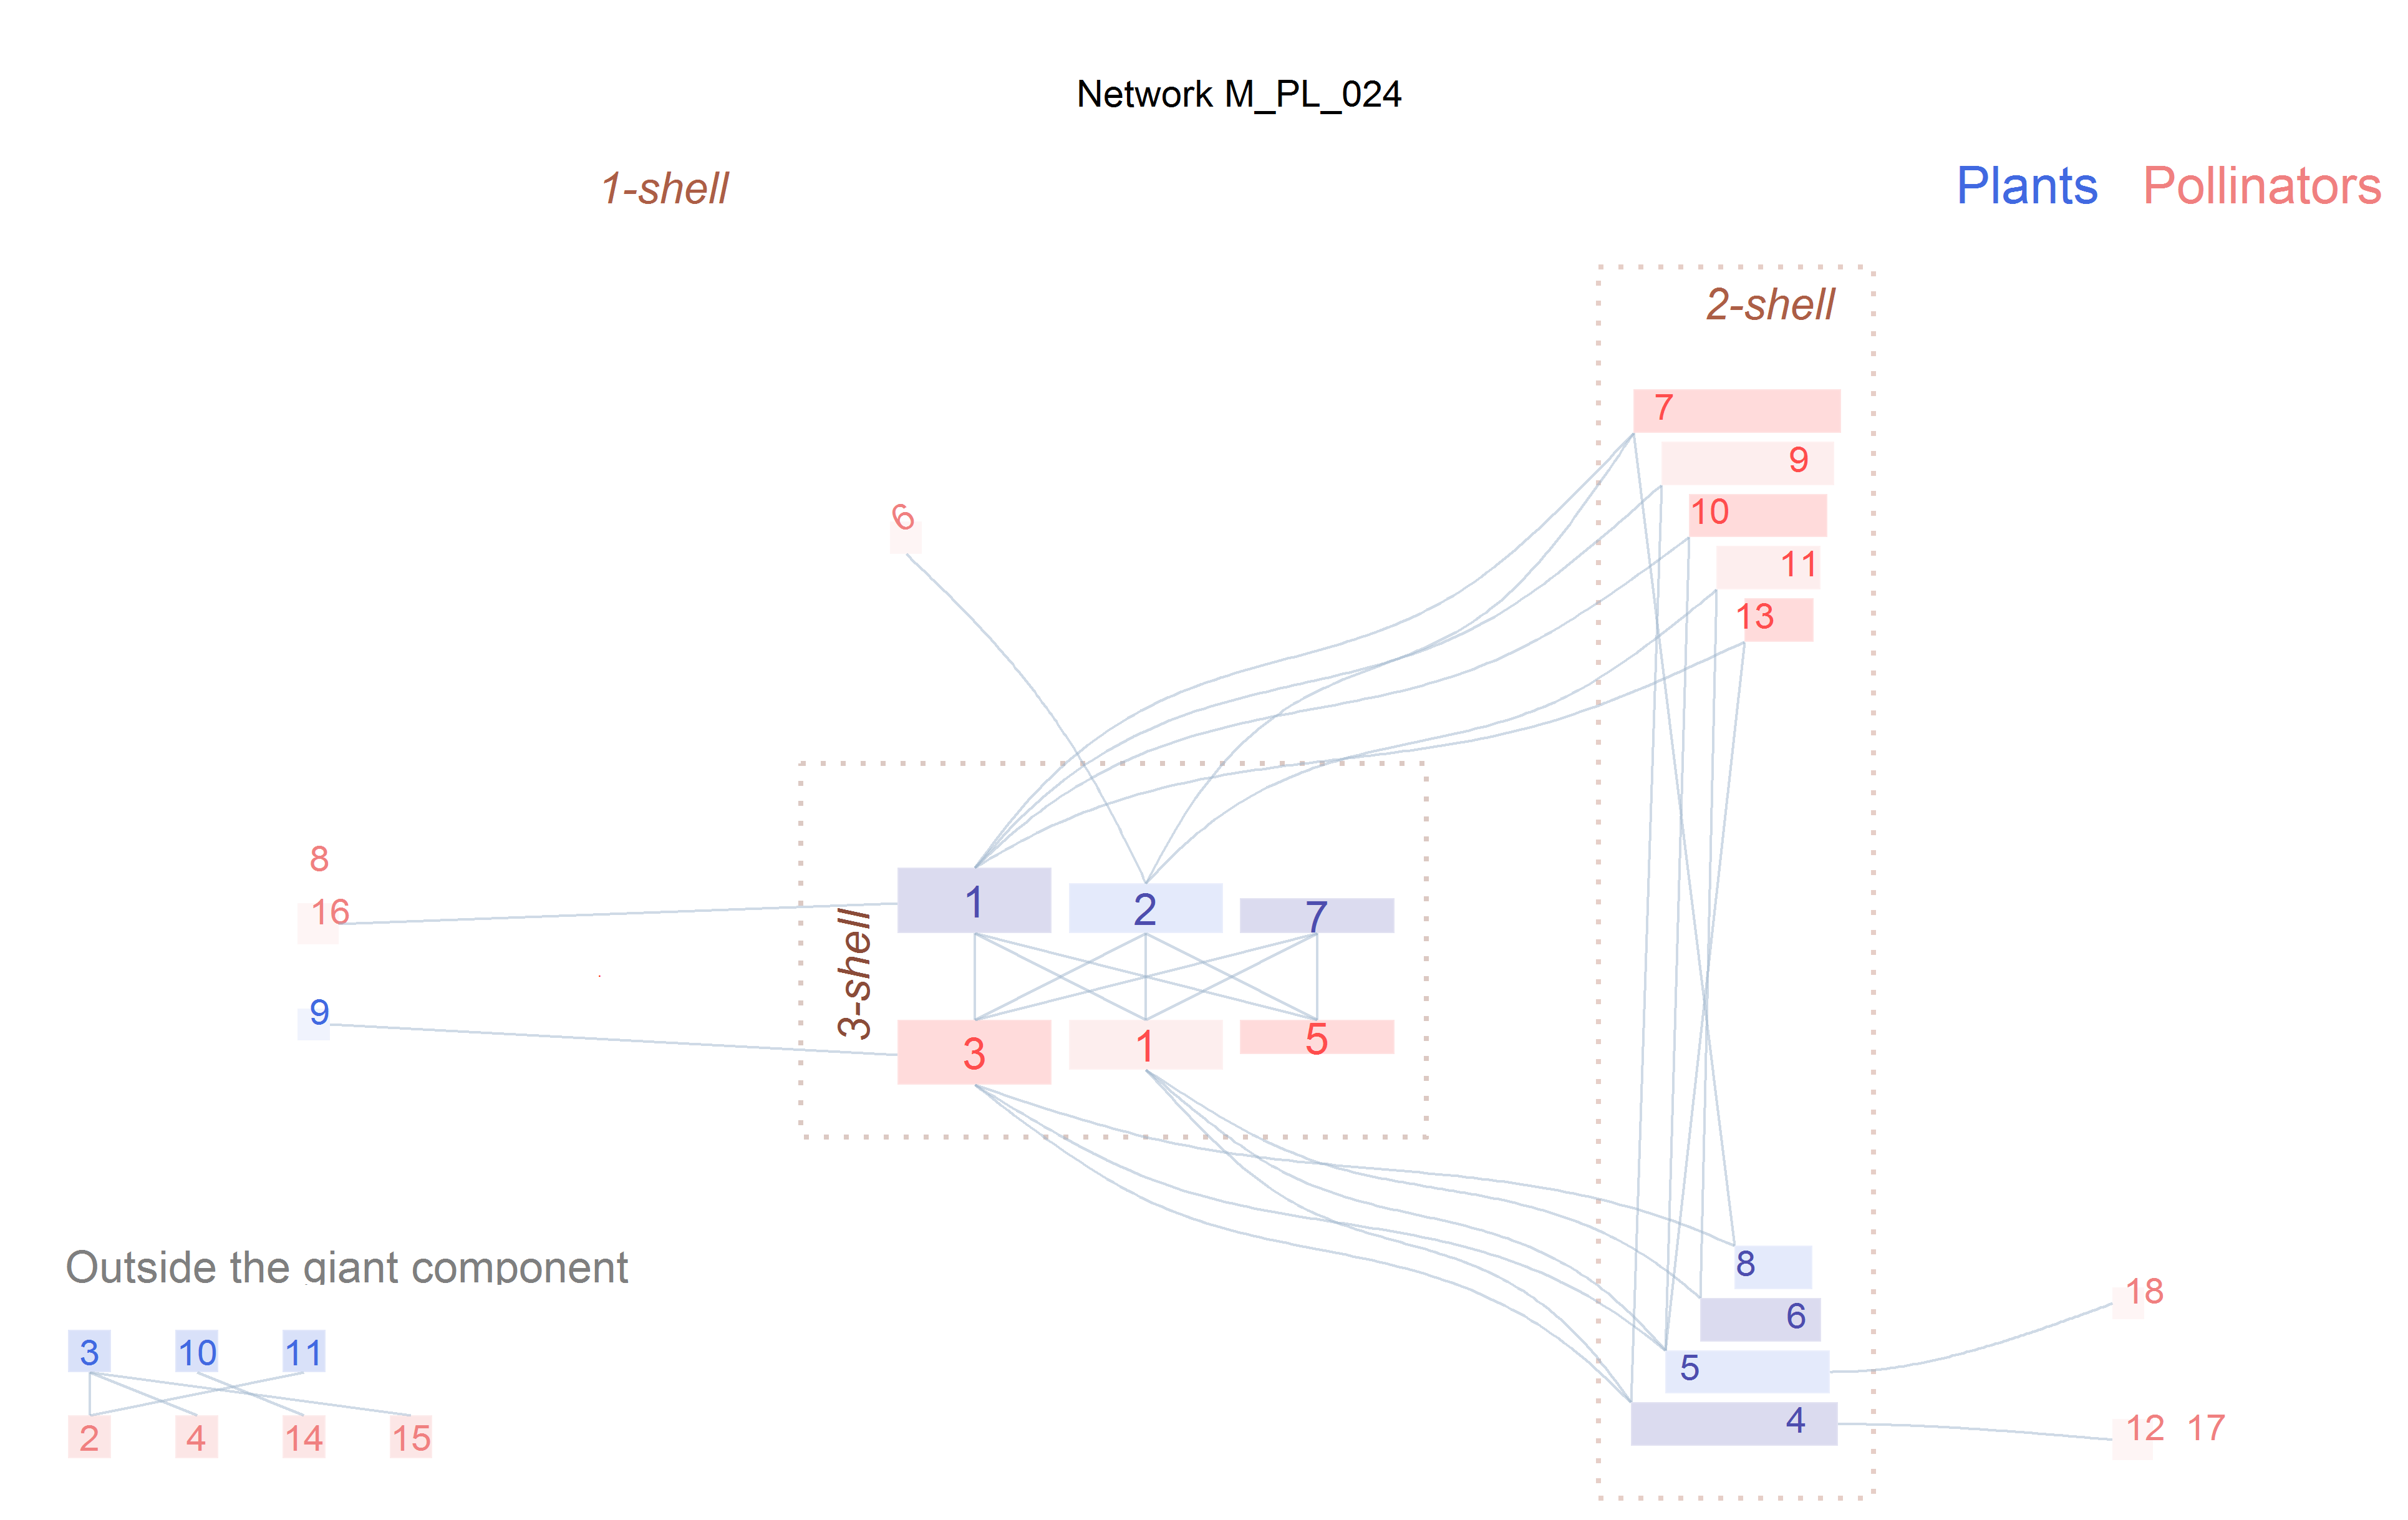
\includegraphics[scale=0.45]{Figures/VIS_M_PL_024_ziggurat.png}
\caption {Red de polinizadores $M\_PL\_024$, Melville Island, Canadá \cite{mosquin1967observations}, con $29$ especies y $38$ enlaces}
\label{fig:VIS_zig_pl_024}
\end{figure}

El diagrama zigurat funciona bien para los tamaños típicos de las redes mutualistas documentadas en la literatura. La red de la figura \ref{fig:VIS_zig_pl_024} es pequeña, muy simétrica y con valores intermedios de $NODF$ y de las \textit{k magnitudes} (véase la tabla \ref{table:table_results}). La especie con mayor $k_{degree}$ $(5,74)$ es la planta $1$. En esta red todas las especies de las \textit{shells} máximas están conectadas entre sí, por lo que sus $k_{radius}$ valen $1,0$, pero esto no tiene por qué suceder siempre. Las más distantes de la $3$-$shell$ (descartando las que no están conectadas con la componente gigante) son los polinizadores $12$, $17$ y $18$, con  $k_{radius}$ $3,0$, que aparecen conectadas al extremo derecho del zigurat de la $2$-$shell$ de plantas.

\begin{figure}[h!]
\centering
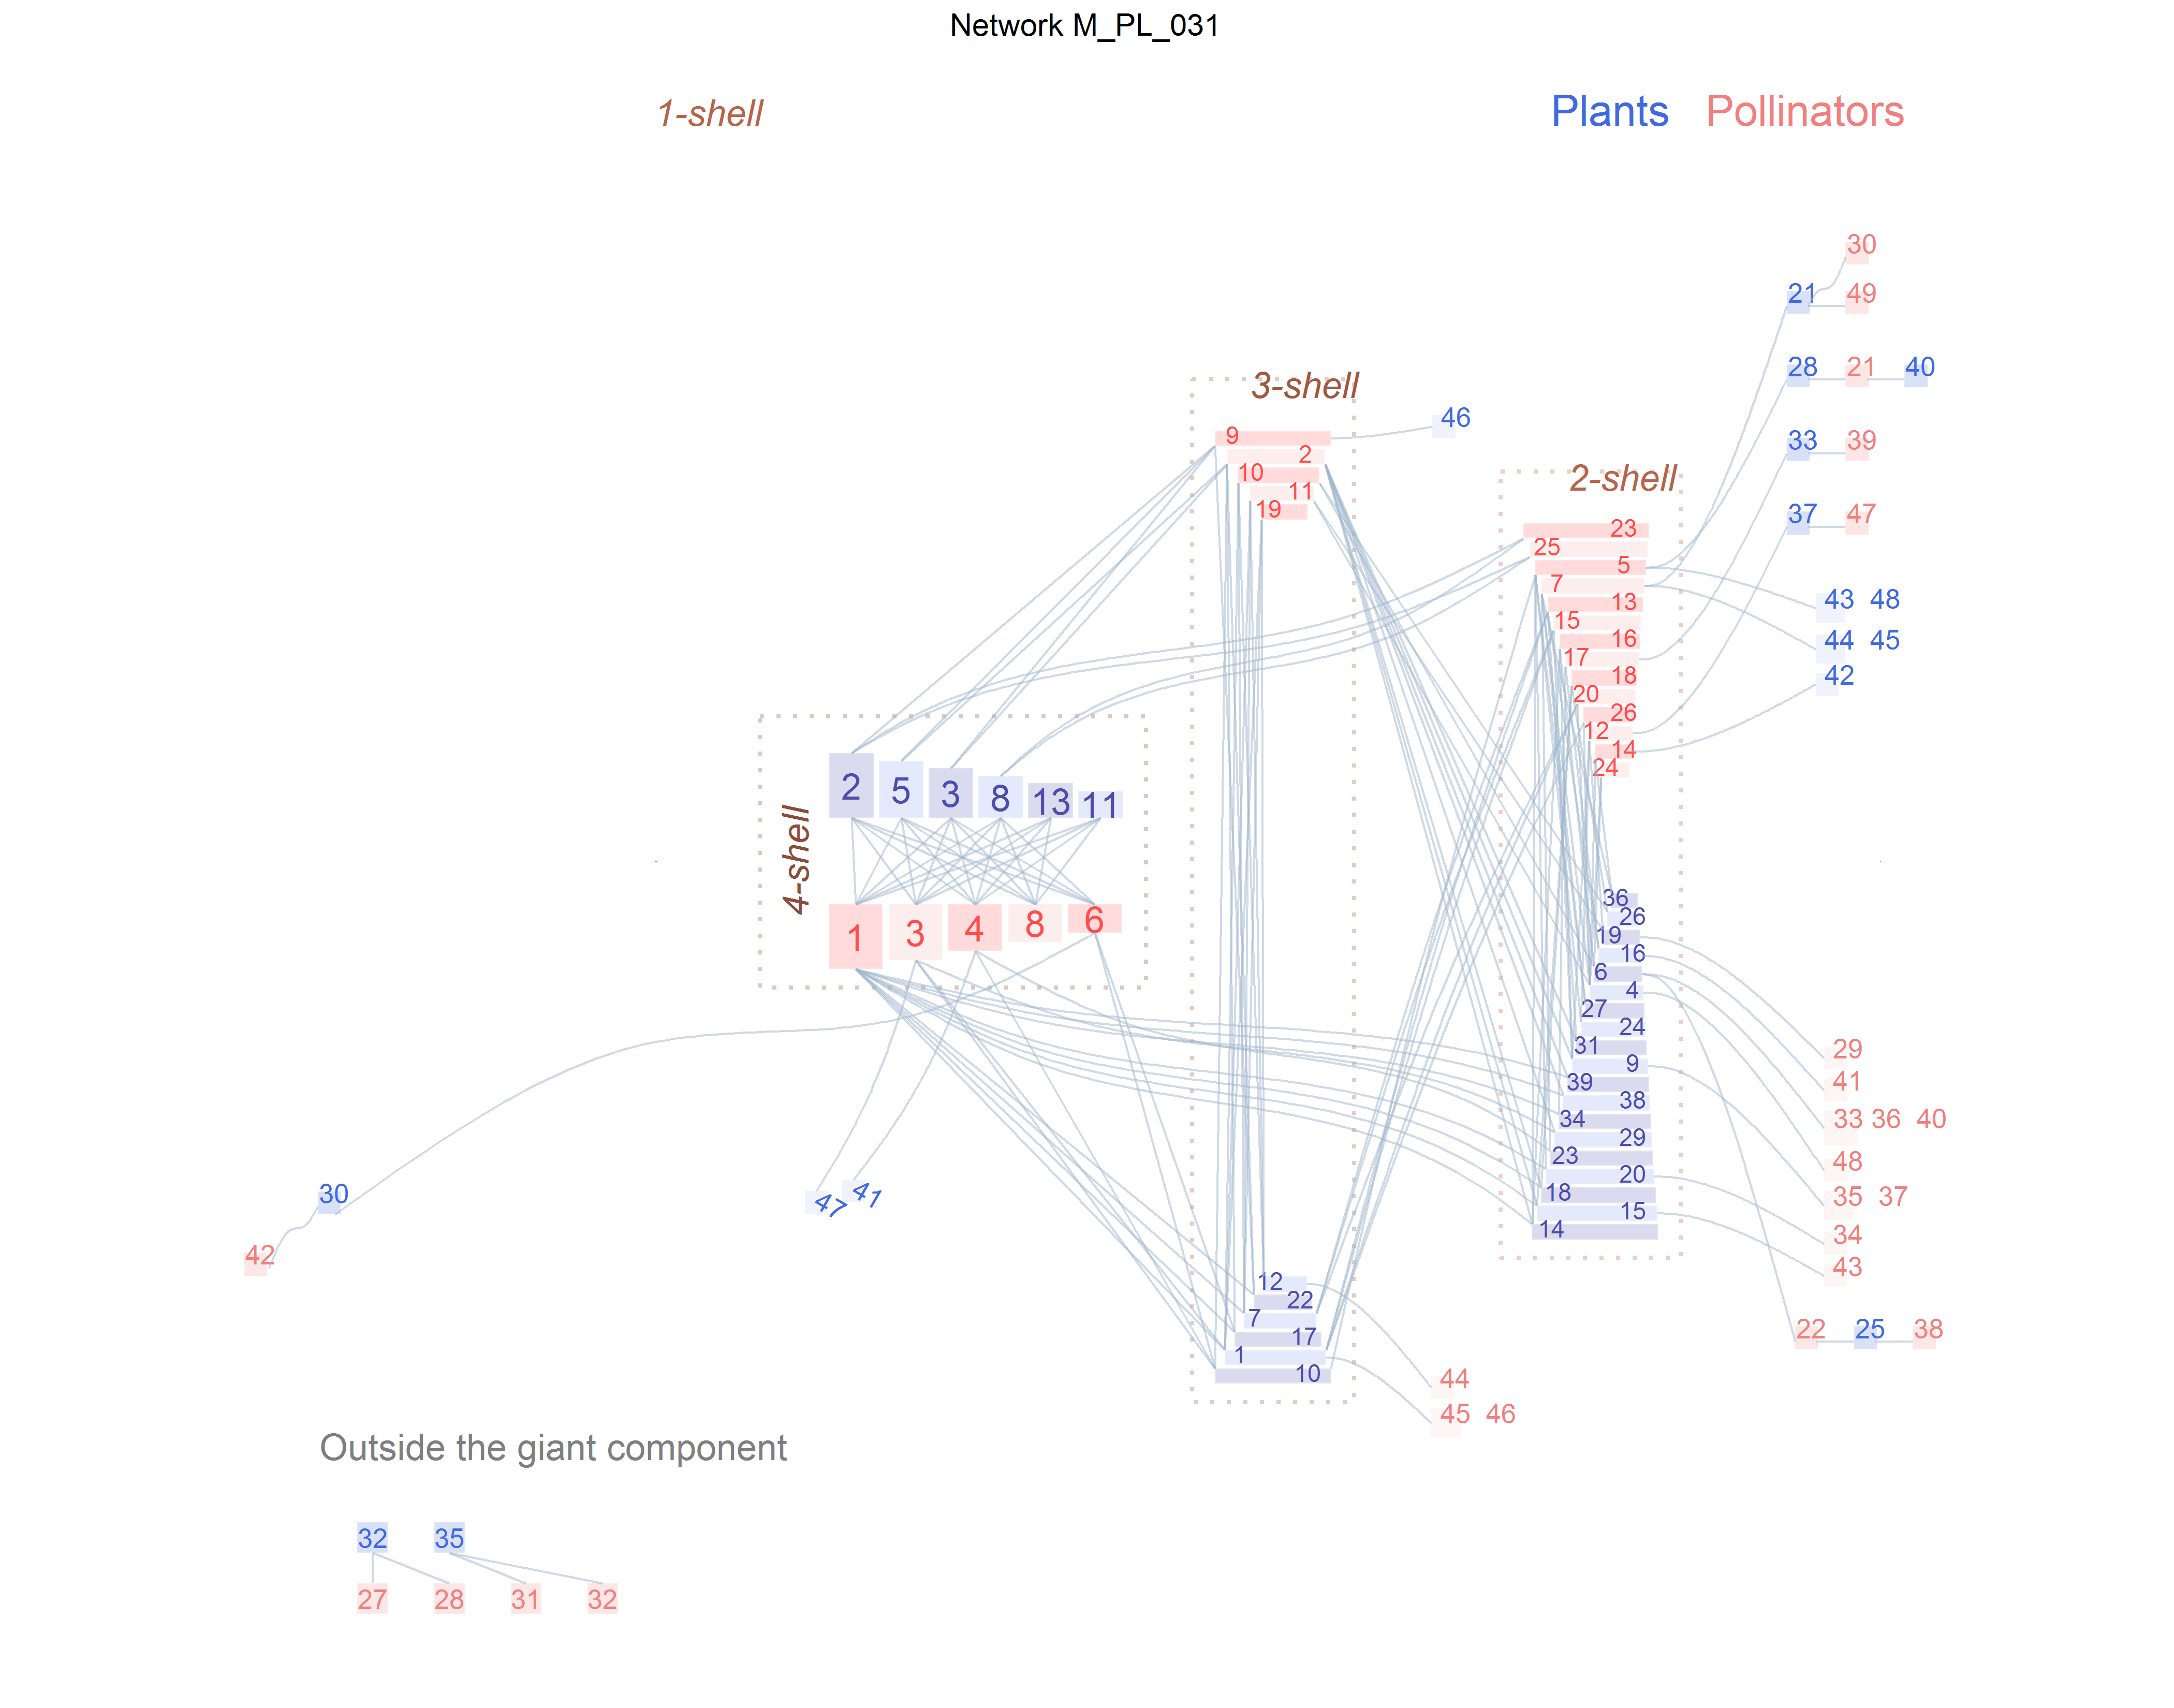
\includegraphics[scale=1]{Figures/VIS_M_PL_031_ziggurat.png}
\caption {Red de polinizadores $M\_PL\_031$ del Parque Nacional de Canaima, Venezuela, con $97$ especies y $156$ enlaces \cite{ramirez1989biologia}.}
\label{fig:VIS_M_PL_031_ziggurat}
\end{figure}

La red de la figura \ref{fig:VIS_M_PL_031_ziggurat} es de un tamaño intermedio, y muestra abundancia de especialistas conectadas a otras especialistas, una circunstancia poco común. A diferencia del caso anterior, no todas las especies del las \textit{shells} máximas tienen enlaces directos con todas las de la clase contraria. Así, mientras el $k_{radius}$ del polinizador $1$ o la planta $2$ es $1,0$, el de la planta $13$ es $1,4$ y el del polinizador $6$ es $1.66$ (tabla \ref{table:kmag_pl_031}). La existencia de especialistas ultraperiféricos se traduce en valores elevados del $k_{radius}$, por ejemplo $7.0$ para el polinizador $38$ ó $6.2$ para la planta $25$ que es el primer enlace de su camino más corto hacia el centro de la red.

\begin{figure}[ht!]
\centering
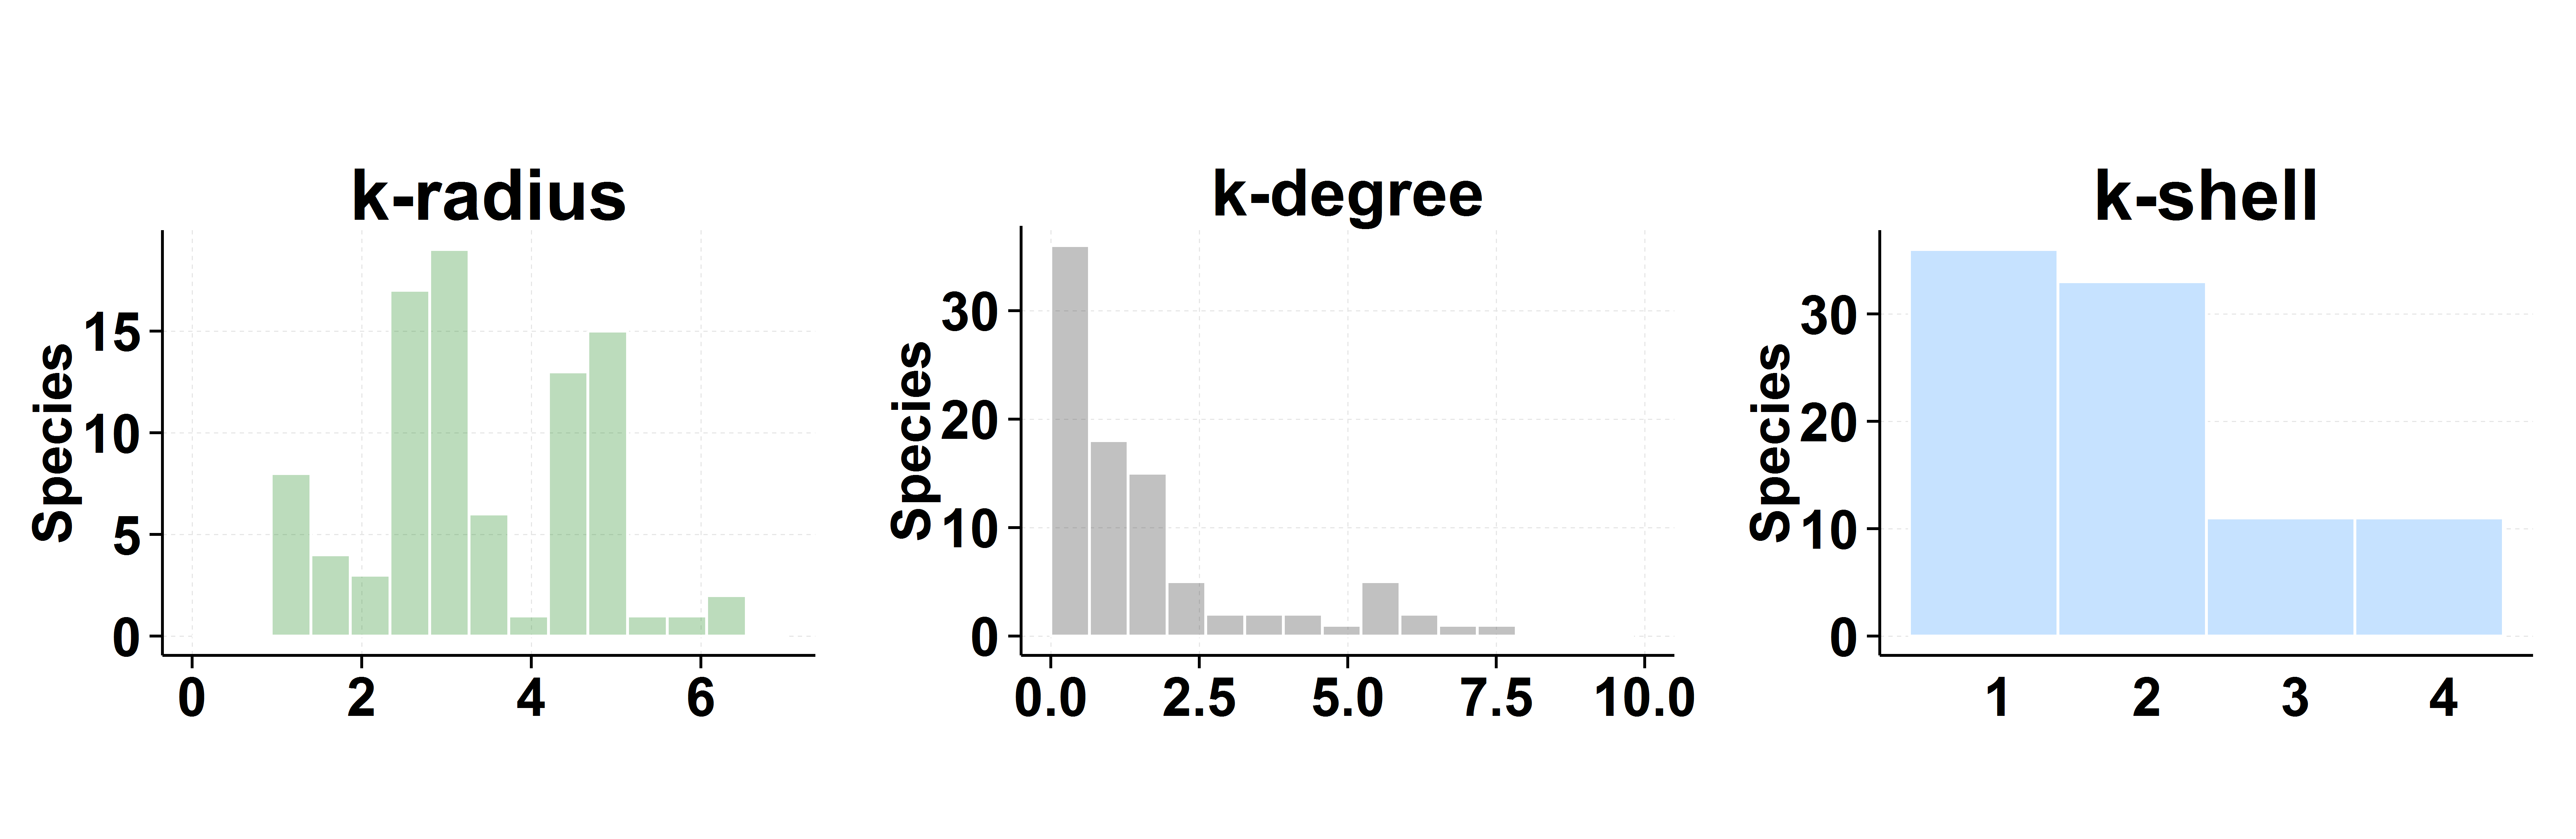
\includegraphics[scale=0.5]{Figures/VIS_M_PL_031_polar.png}
\caption {Histograma de las \textit{k magnitudes} de polinizadores del Parque Nacional de Canaima, Venezuela \cite{ramirez1989biologia}.}
\label{fig:VIS_M_PL_031_polar}
\end{figure}

Estas especies tan alejadas del centro corren el peligro de extinción por arrastre que se describió en el apartado \ref{results_K_constante}. Supongamos que el polinizador número $7$ se extingue por una plaga. En la parte superior derecha de la figura \ref{fig:VIS_M_PL_031_ziggurat} puede verse la tripleta planta $21$, polinizadores $30$ y $49$ que quedarían desconectados de la componente gigante y posiblemente se extinguirían también. En el mejor de los casos, si por el peso de sus enlaces superaran el mínimo vital de la nueva red formada por las tres, podrían sobrevivir aisladas pero mucho más expuestas a cualquier perturbación posterior. Las plantas $44$ y $45$ desaparecerían con seguridad porque el polinizador $7$ es su única especie benefactora. De esta manera, la destrucción de un polinizador podría arrastrar cinco especies más a la extinción. En el diagrama se puede ver también la gran conectividad entre especies de las \textit{shells} de índices $2$ y $3$, lo que reduce el anidamiento bajo y aumenta la modularidad. Por el contrario, la red de la figura \ref{fig:ziggurat} es mucho más anidada, con pocos enlaces que no terminen en la $4$-$shell$ y compacta, con un $\overline k_{radius}$ reducido ($2,19$ frente a $3,39$).


El tamaño de una red se puede medir en número de nodos o en número de enlaces, pero es esta segunda cifra la que predomina a la hora de fijar la complejidad de la estructura de \textit{k shells}. La red de la figura \ref{fig:VIS_M_PL_010_ziggurat}, tiene $107$ especies y $456$ enlaces y su índice $k$ máximo es $8$. Se aprecia asimetría importante con predominio de los polinizadores. En contraste con los ejemplos anteriores, hay muy pocas especies que pertenezcan a la $1$-$shell$. Las conexiones entre las distintas \textit{shells} forman un entramado visualmente complejo.

Con menos especies $(85)$ y solo un $10\%$ más de enlaces, la comunidad de frugívoros de la selva malaya de la figura \ref{fig:VIS_M_PL_047_ziggurat}, tiene un índice $k$ máximo de $11$, ninguna otra de la colección \textit{web of life} lo alcanza. Es muy asimétrica y el valor de $\overline k_{degree}$ es excepcional ($8,4$), por la circunstancia de tener ese $k$ máximo, la elevada conectividad de las especies y su cercanía a la $11$-$shell$.

La red de polinizadores de un brezal danés (figura \ref{fig:VIS_M_PL_047_ziggurat}), tiene $205$ especies y $425$ enlaces. El $k$ máximo es solo $6$. La asimetría es también muy marcada pero lo que más destaca es la extraordinaria cantidad de polinizadores en la $1$-$shell$. Con este ejemplo se aprecia mejor el valor de agrupar todas las especies de la $1$-$shell$ que se conectan a una especie de las \textit{shells} más internas y dibujar solo un enlace. 

\begin{figure}[ht!]
\centering
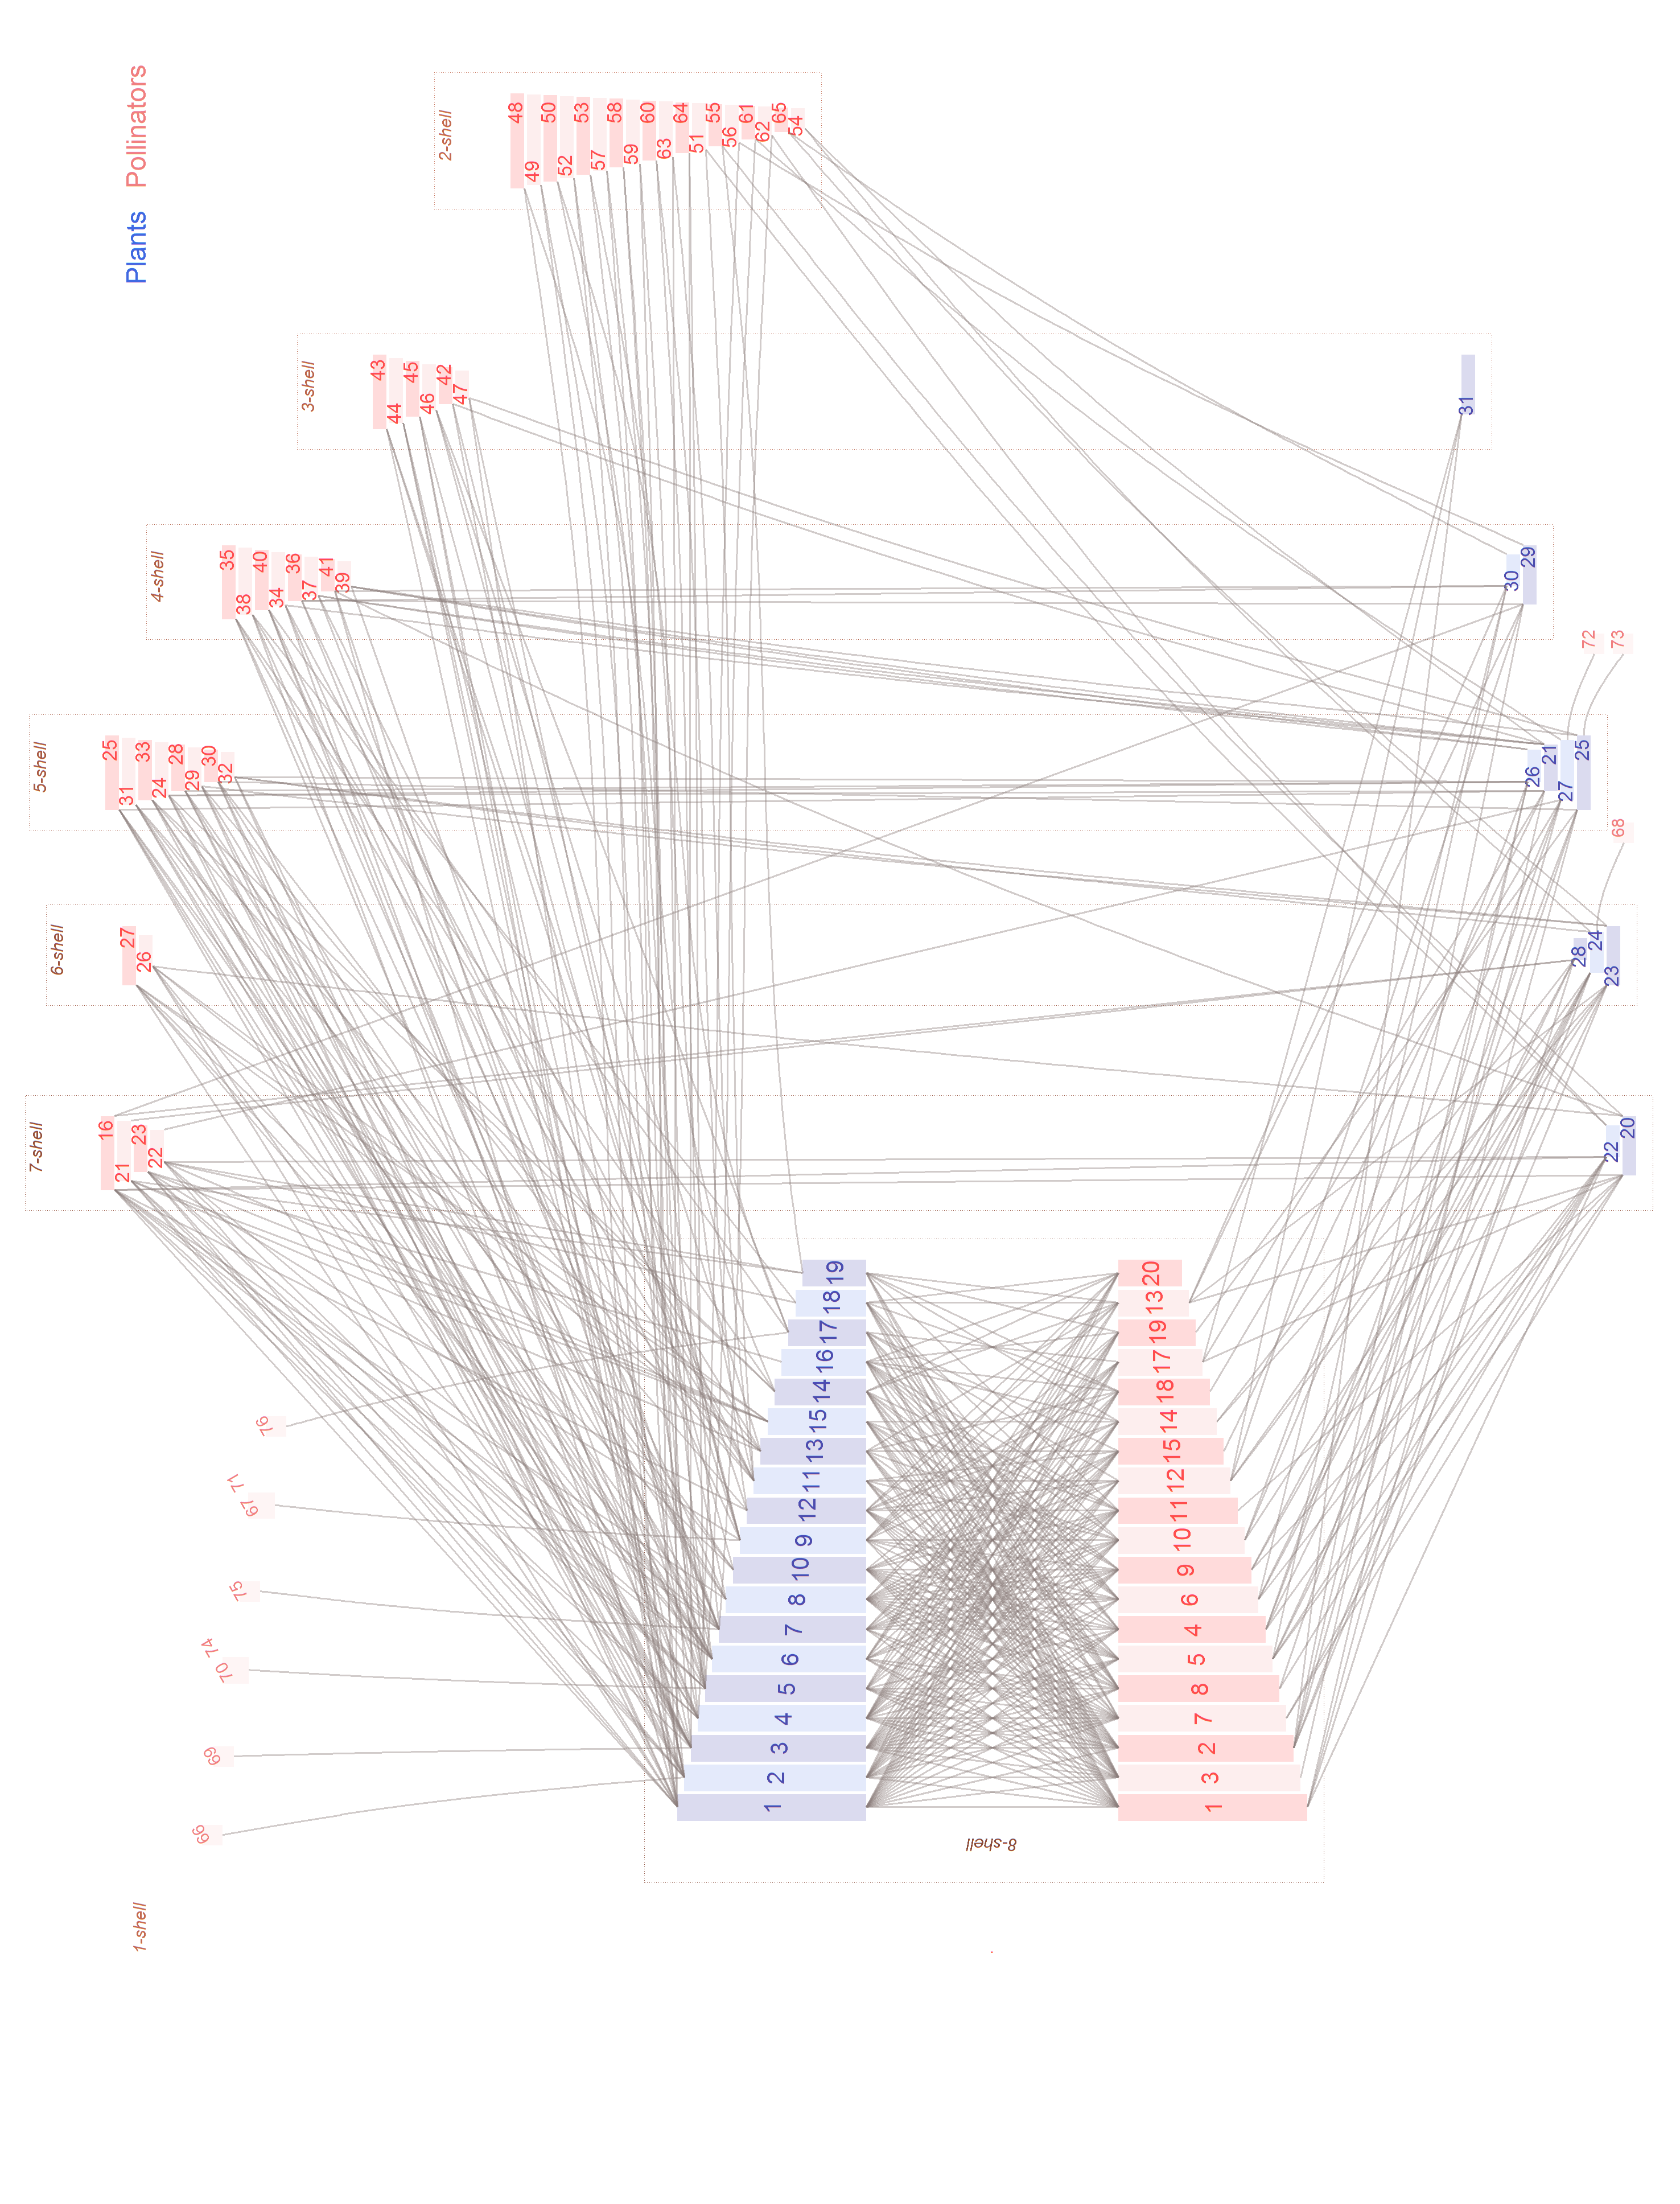
\includegraphics[scale=0.5]{Figures/VIS_M_PL_010_ziggurat.png}
\caption {Red de polinizadores $M\_PL\_010$ (Elberling \& Olesen, no publicada), con $107$ especies y $456$ enlaces. Su diagrama polar puede verse en la figura \ref{fig:VIS_Modvskdegree3}.}
\label{fig:VIS_M_PL_010_ziggurat}
\end{figure}

\clearpage
\begin{figure}[ht!]
\centering
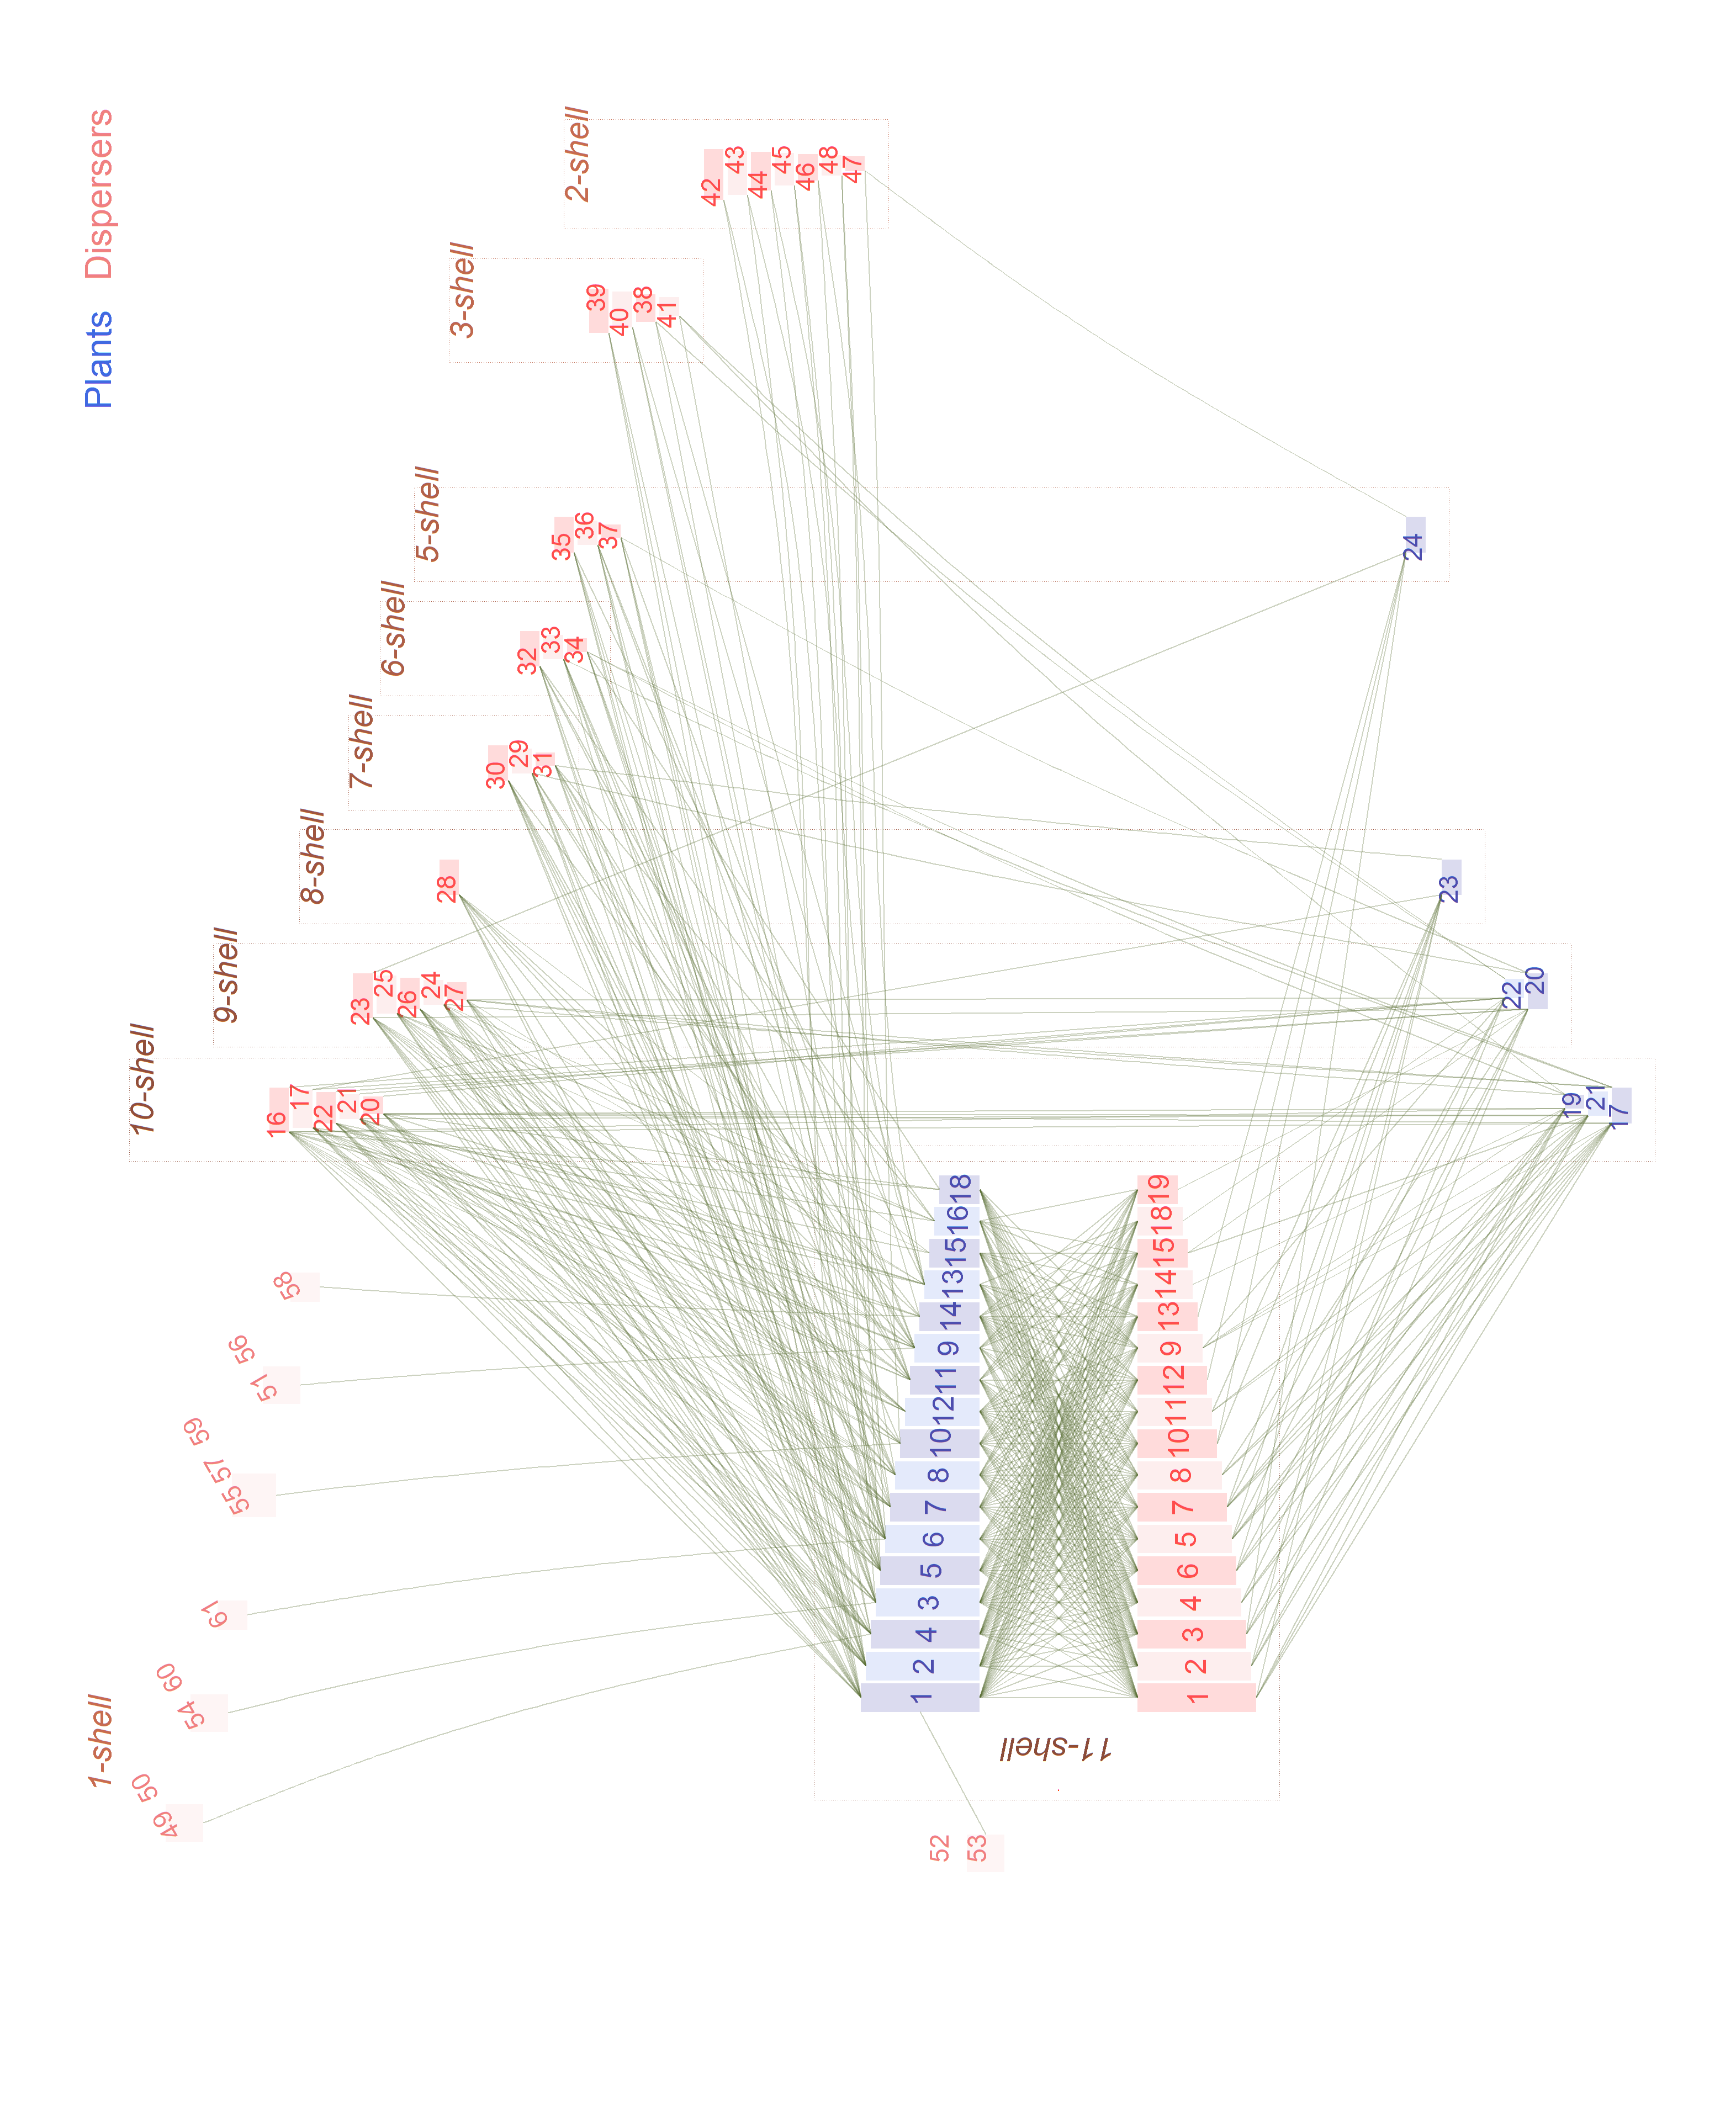
\includegraphics[scale=0.20]{Figures/VIS_M_SD_016_ziggurat.png}
\caption {Red de aves frugívoras $M\_SD\_016$ en la selva Kuala Lompat, Reserva de Krau Game, Malasia \cite{lambert1989fig}, con $85$ especies y $500$ enlaces.}
\label{fig:VIS_M_SD_016_ziggurat}
\end{figure}

\clearpage
\begin{figure}[ht!]
\centering
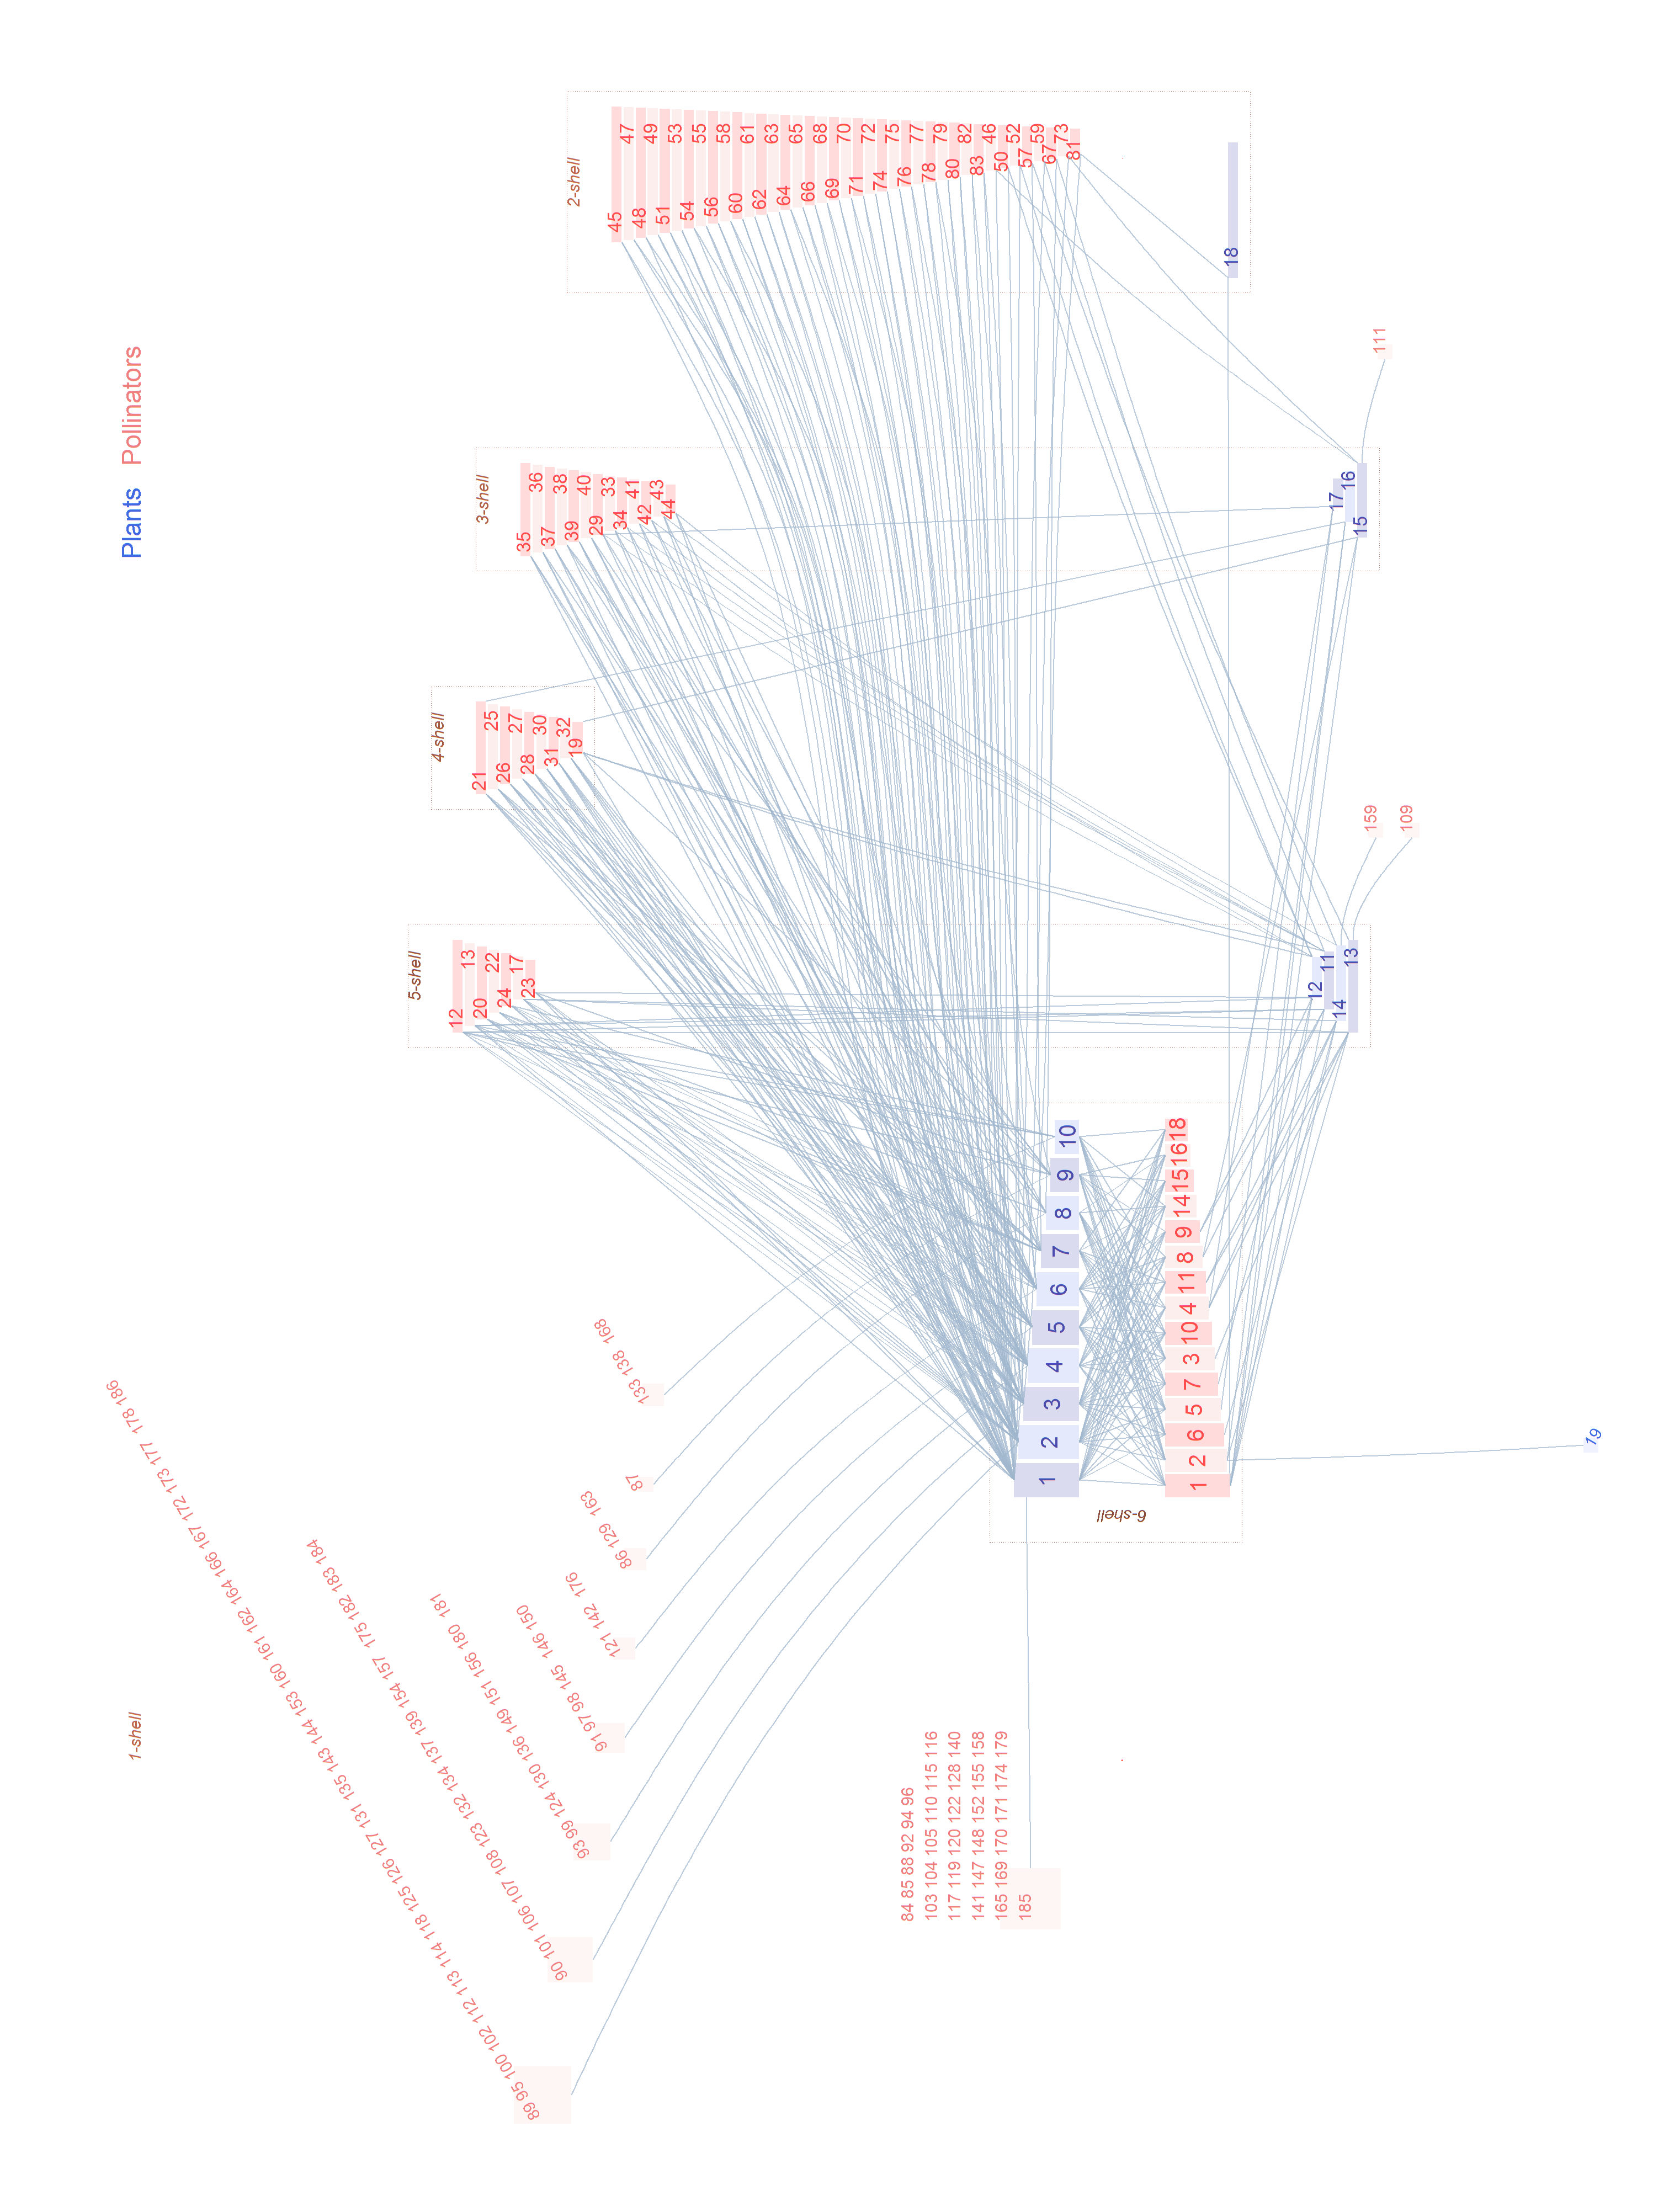
\includegraphics[scale=0.20]{Figures/VIS_M_PL_047_ziggurat.png}
\caption {Red de polinizadores $M\_PL\_047$, de un brezal en Isen Bjerg, Dinamarca \cite{dupont2009ecological}, con $205$ especies y $425$ enlaces.}
\label{fig:VIS_M_PL_047_ziggurat}
\end{figure}


\clearpage
\section{Visualización de la estructura}

El diagrama zigurat no solo sirve para captar la riqueza y variedad de las comunidades mutualistas, también puede ayudar a entender algunas de sus propiedades. En el capítulo precedente se llevó a cabo un análisis de modelo nulo que reveló importantes diferencias en las redes de la colección \ref{fig:ESTATICA_zscore_all}. Se comprobó que la mayoría de las que tienen matriz de adyacencia pesada no son significativamente anidadas usando un modelo nulo restrictivo. Pese a ello, tres sí mostraban fuerte anidamiento y una de ellas además era compacta, la red de polinizadores $059$ (figura \ref{fig:VIS_M_PL_059_ziggurat}).

\begin{figure}[h!]
\centering
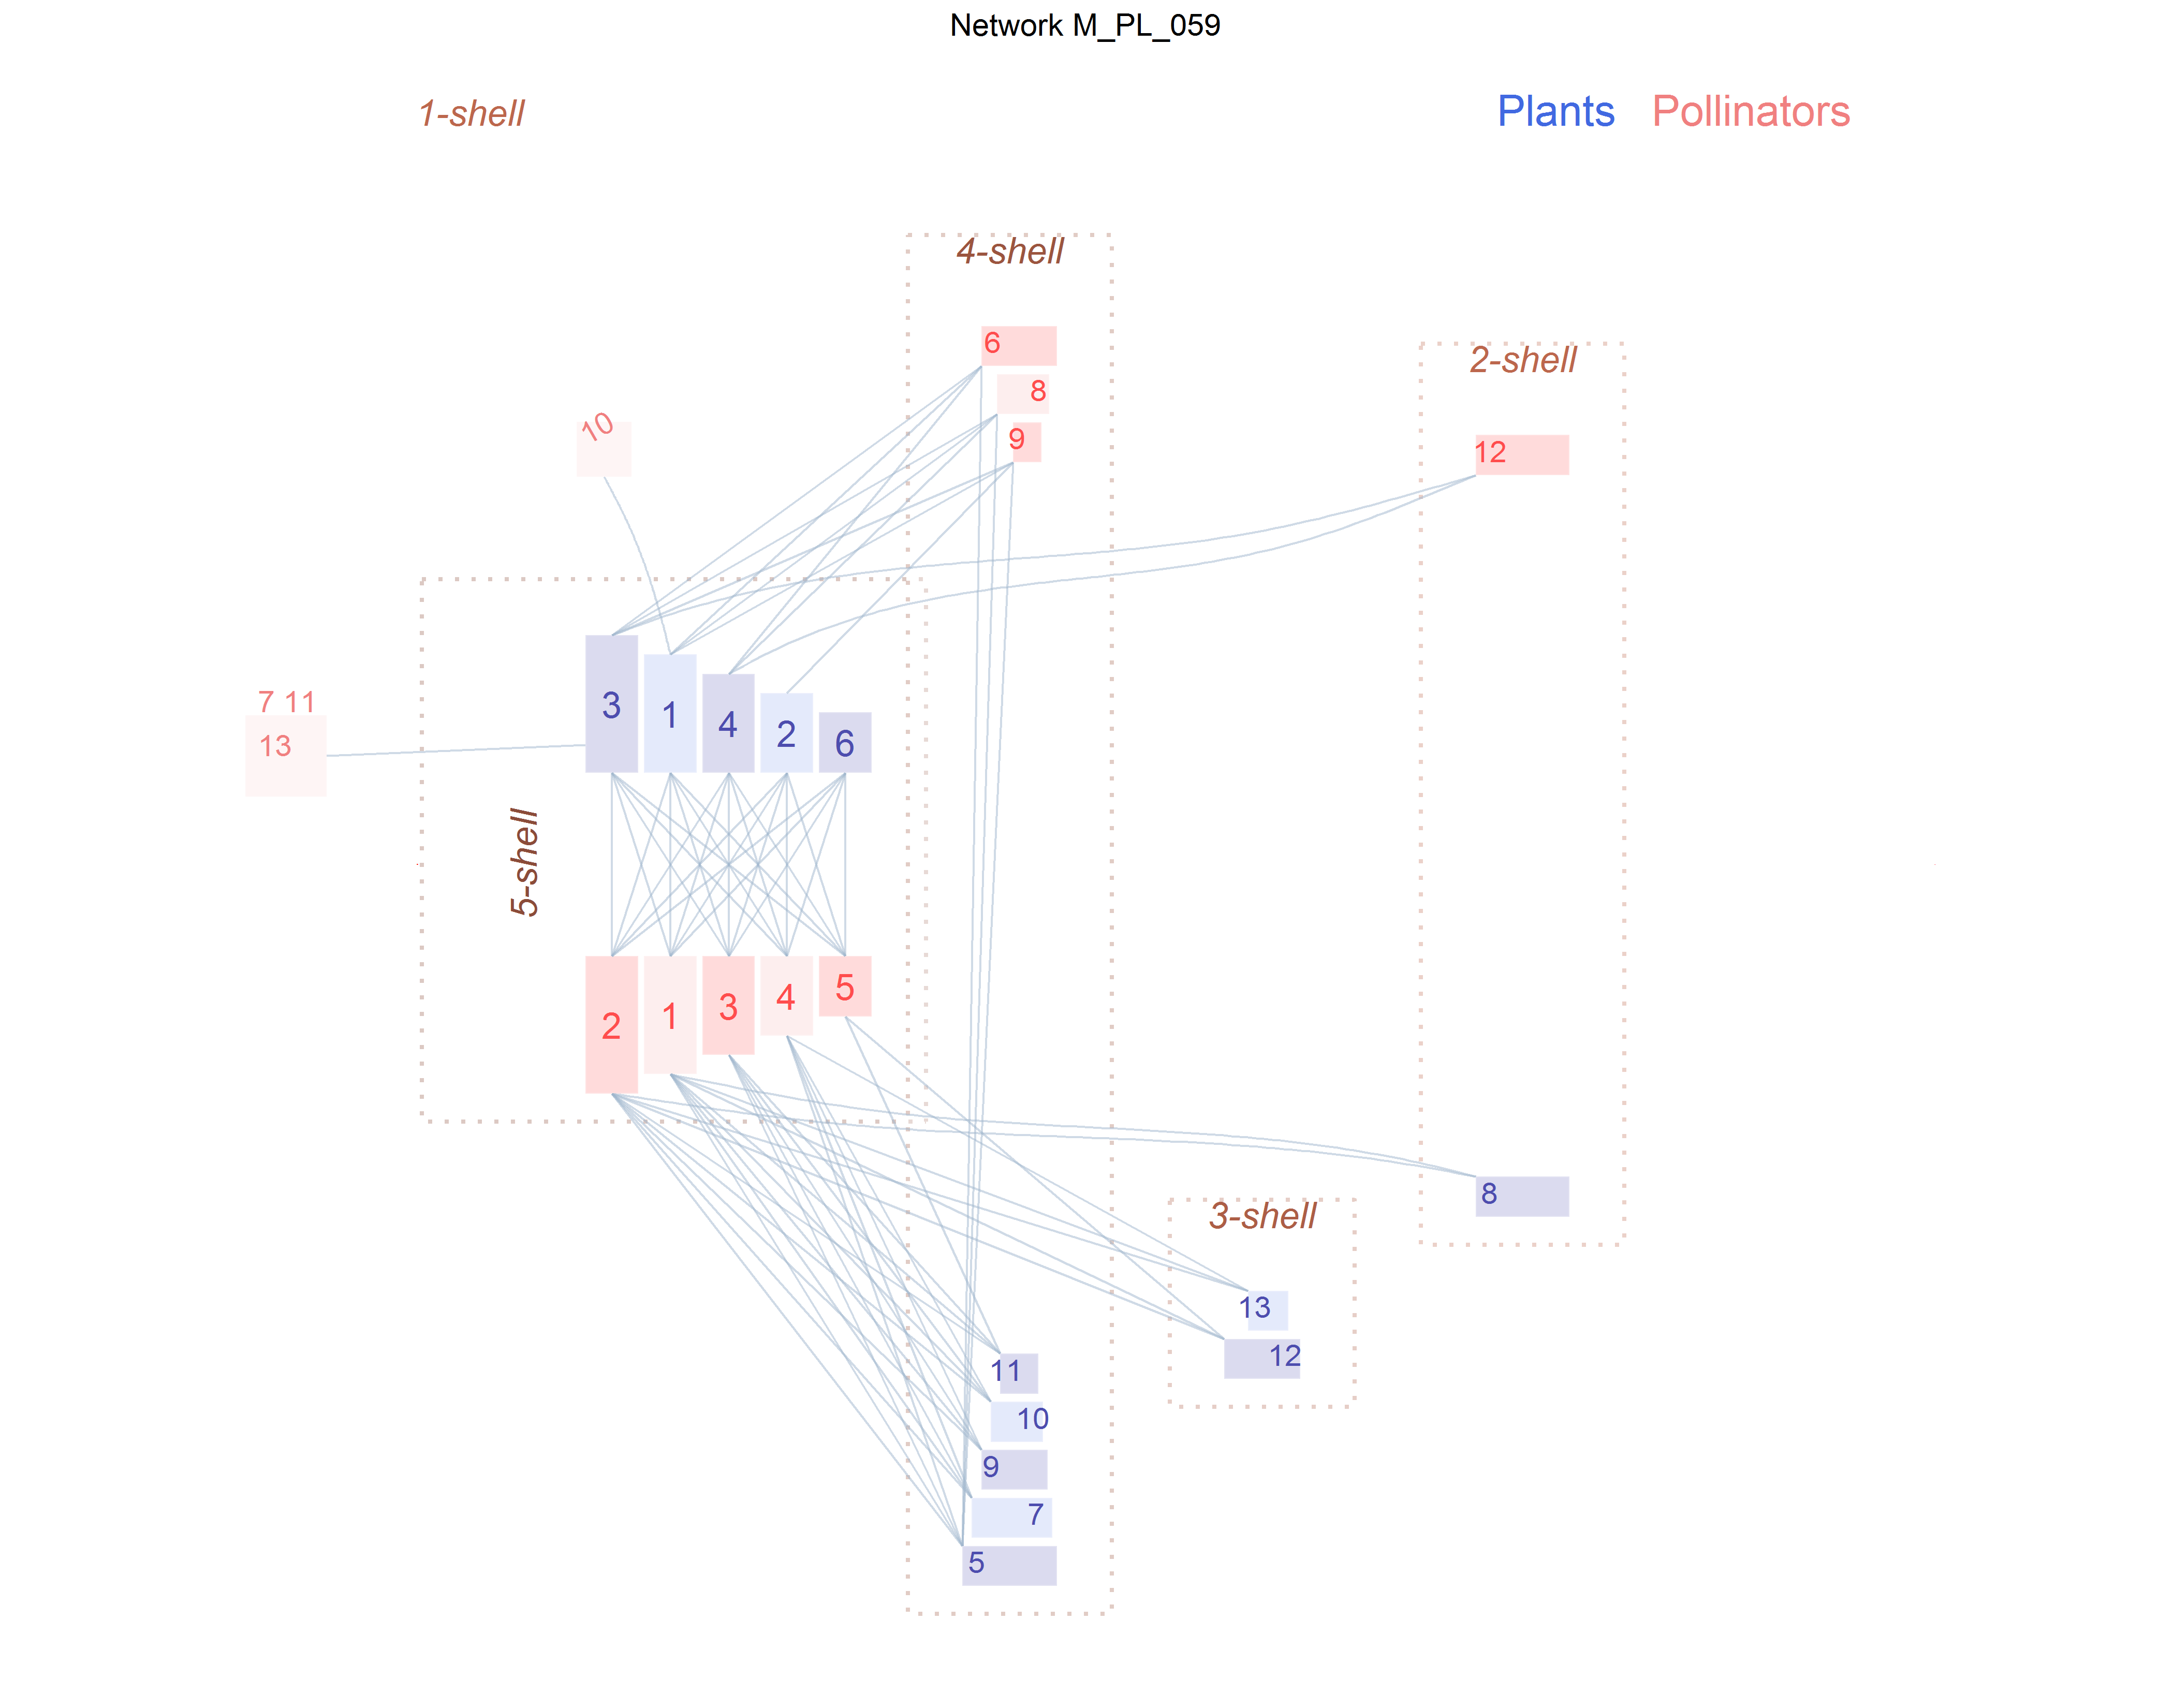
\includegraphics[scale=0.42]{Figures/VIS_M_PL_059_ziggurat.png}
\caption {Red de polinizadores $M\_PL\_059$, Parque Nacional do Catimbau, Brasil, con $26$ especies y $71$ enlaces \cite{bezerra2009pollination}. $NODF = 76,88$, $\overline {k}_{radius} = 1,57$ .}
\label{fig:VIS_M_PL_059_ziggurat}
\end{figure}

Con este gráfico se entiende fácilmente por qué $zNODF = 6,84$ y $z \overline {k}_{radius} = -7,34$ alcanzan valores tan extremos. Todas las especies tienen enlaces directos con la \textit{shell} máxima y apenas hay $3$ enlaces entre nodos de la $4$-$shell$. Es un caso de anidamiento y compacidad altísimos.

La red $M\_PL\_024$ (figura \ref{fig:VIS_zig_pl_024}) no es anidada ($zNODF = -1,79$) pero está al límite de ser compacta ($\overline {k}_{radius} = -1,98$). Esta configuración, con forma de campanilla recostada, es bastante habitual y aparece en los procesos de destrucción. Hay un número no despreciable de enlaces dentro de la $2$-$shell$. Esto reduce el valor del anidamiento, pero no afecta al ${k}_{radius}$ de las especies porque tienen también conexión directa con la \textit{shell} máxima.

Entre las redes con matriz binaria la que se sitúa en el extremo de máximo anidamiento y compacidad en la de dispersores de semillas número $016$ (figura \ref{fig:VIS_M_SD_016_ziggurat}). La hemos utilizado como ejemplo en el apartado anterior y es patente como una gran mayoría de los enlaces tienen extremo en la $11$-$shell$. Por esto, los índices reducidos toman también
valores excepcionales: $zNODF = 16,65$ y $\overline {k}_{radius} = -7,99$.

En el extremo opuesto se encuentra la red de polinizadores $031$ (figura \ref{fig:VIS_M_PL_031_ziggurat}), debido a su peculiar configuración de cadenas de especialistas, que hacen que sea anidada ($zNODF = 3,98$), pero no compacta ($\overline {k}_{radius} = 0,22$). Un caso interesante es el de las redes en las que el índice $k$ máximo es $2$, como la de polinizadores número $022$. Son también anidadas ($zNODF = 3,93$) pero no compactas ($\overline {k}_{radius} = 0,58$).

\begin{figure}[h!]
\centering
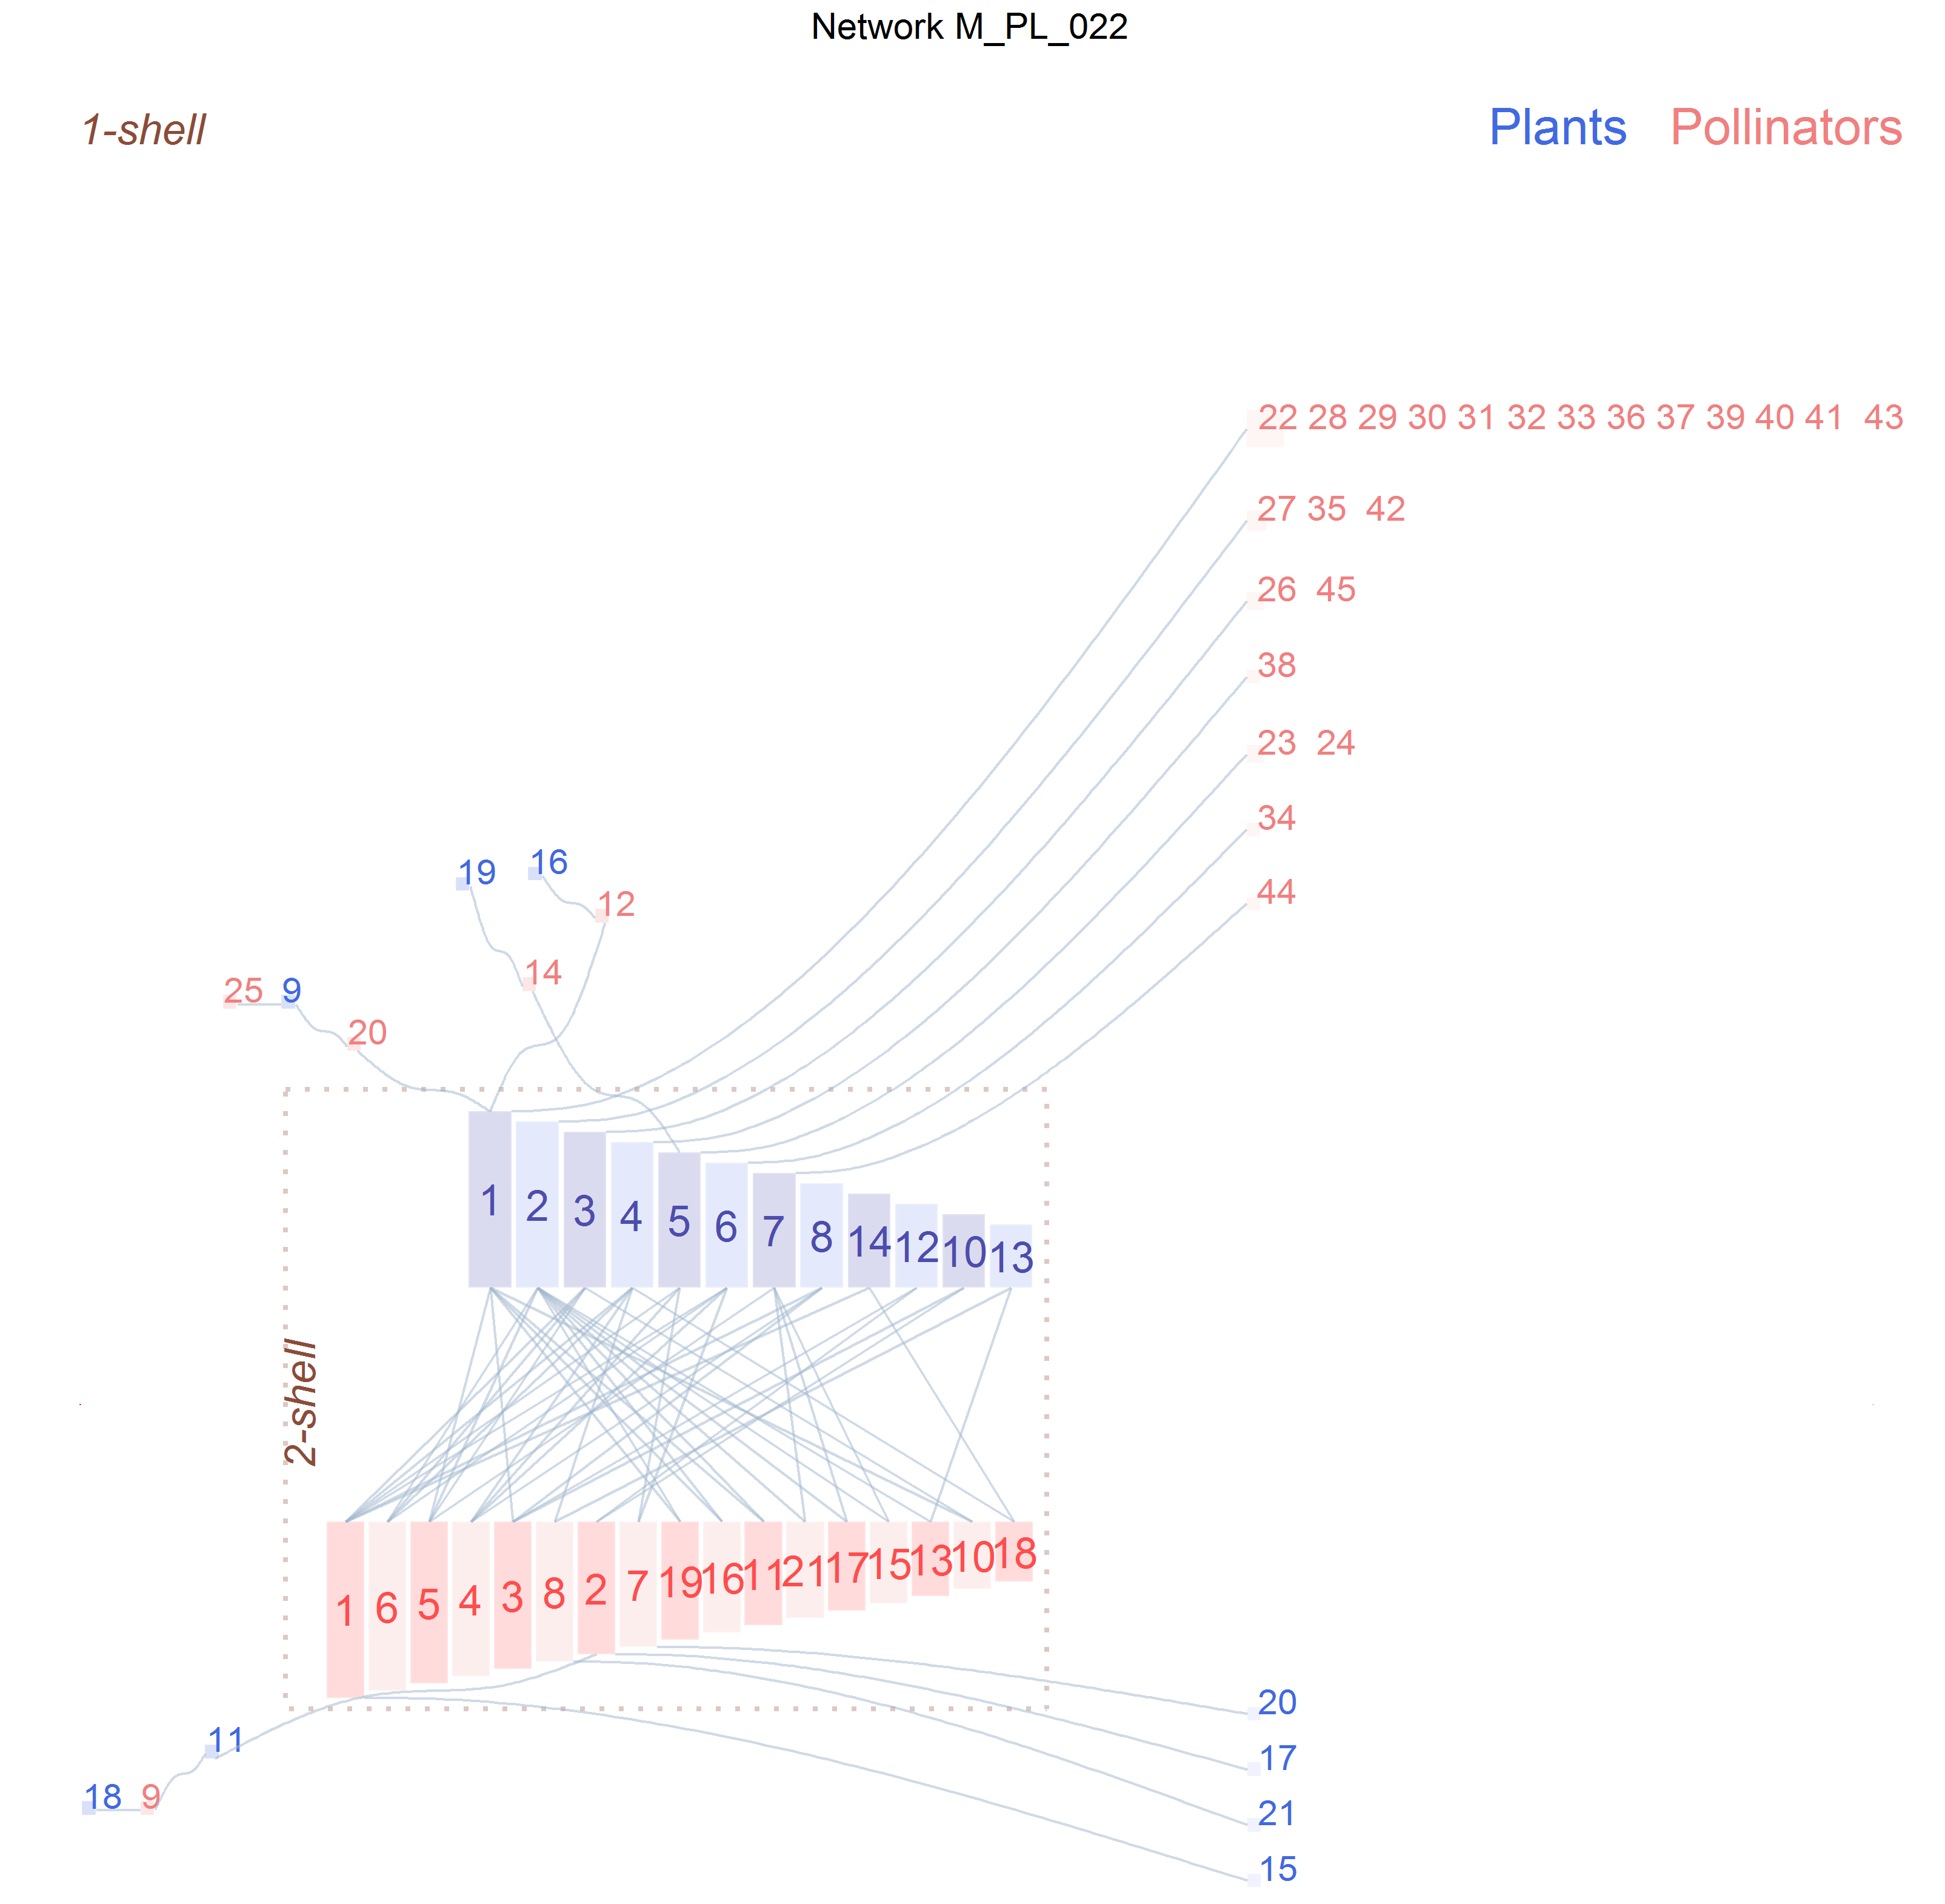
\includegraphics[scale=0.5]{Figures/VIS_M_PL_022_ziggurat.png}
\caption {Red de polinizadores $M\_PL\_022$, Los Andes, Argentina, con $66$ especies y $83$ enlaces \cite{medan2002plant}. $NODF = 18,02$, $z \overline {k}_{radius} = 3,68$ .}
\label{fig:VIS_M_PL_022_ziggurat}
\end{figure}

\clearpage
En el capítulo anterior también se describió un experimento que consiste en recablear al azar un porcentaje de los enlaces y medir su efecto en la correlación entre $NODF$ y $\overline k_{radius}$ (figura \ref{fig:ESTATICA_histo_corr_rewiring}). La mayoría de las redes experimentan una degradación lineal por la que el anidamiento, medido con $NODF$, decrece y el $\overline k_{radius}$ aumenta. Se llega a un estado similar al que se obtendría si las especies interactuasen al azar, lo que sabemos que está lejos de la realidad.

No obstante, un pequeño porcentaje se salía de este patrón. En general, eran redes pequeñas o con una marcada asimetría. En los dos ejemplos que se incluyen a continuación, los diagramas zigurat permiten entender el por qué de este comportamiento.

El primero (figura \ref{fig:VIS_PL_012}) corresponde a una red de tamaño mediano, con una estructura compleja. La red original se representa con los colores habituales, las correspondientes a los distintos grados de recableado en otros tonos, para recalcar que no se trata de redes reales. 

En la red sin alterar, se observa un índice $k$ máximo de $4$, y una gran conectividad directa con esas \textit{shells}. Hay un importante número de especies en la $1$-$shell$. En el gráfico de correlación general entre $NODF$ y $\overline k_{radius}$ (figura \ref{fig:ESTATICA_corrfigs}) esta red se sitúa en una zona intermedia.

Cuando se reconectan al azar seis enlaces, la estructura cambia poco, aunque puede verse como aparece una $2$-$shell$ de plantas y aumenta la conectividad entre las \textit{k shells} inferiores. Es importante recalcar que esta red alterada es resultado de una realización aleatoria, la configuración puede variar entre distintos intentos, por eso las gráficas de la figura \ref{fig:ESTATICA_corrfigs} se obtuvieron repitiendo veinte veces el recabledado para un mismo número de enlaces. No obstante, un recableado mínimo como el del ejemplo, tiene pocas consecuencias para las medidas globales de esta red.

Al aumentar a diecisiete los enlaces reconectados, la degradación es más notable. El índice $k$ máximo baja a $3$. Si sigue creciendo la cantidad de reconexiones, la modificación es aun más evidente. En la imagen, para treinta y dos cambios al azar, las $2$-$shells$ han crecido a costa de la $3$ y aparecen muchas más conexiones, en proporción, entre ellas. La $NODF$ ha bajado desde el original $30,40$ a $12,22$ y el $\overline k_{radius}$ pasa de $2,51$ a $2,82$.

Obsérvese la forma de campanilla recostada que revela el diagrama zigurat de la red con la mitad de sus enlaces recableados, con  muchas conexiones entre especies de la $2$-$shell$. Esta figura es la de una red mutualista poco estructurada.

En el segundo ejemplo se presenta un caso extremo de comportamiento fuera de la norma  (figura \ref{fig:VIS_SD_007}). Esta red de frugívoros es muy asimétrica con solo $7$ especies de plantas por $72$ de animales. Las especies $1$ a $6$ de plantas forman la $3$-$shell$, solo la número $7$ tiene un lugar marginal en la $1$-$shell$.

\clearpage
\begin{figure}[ht!]
\centering
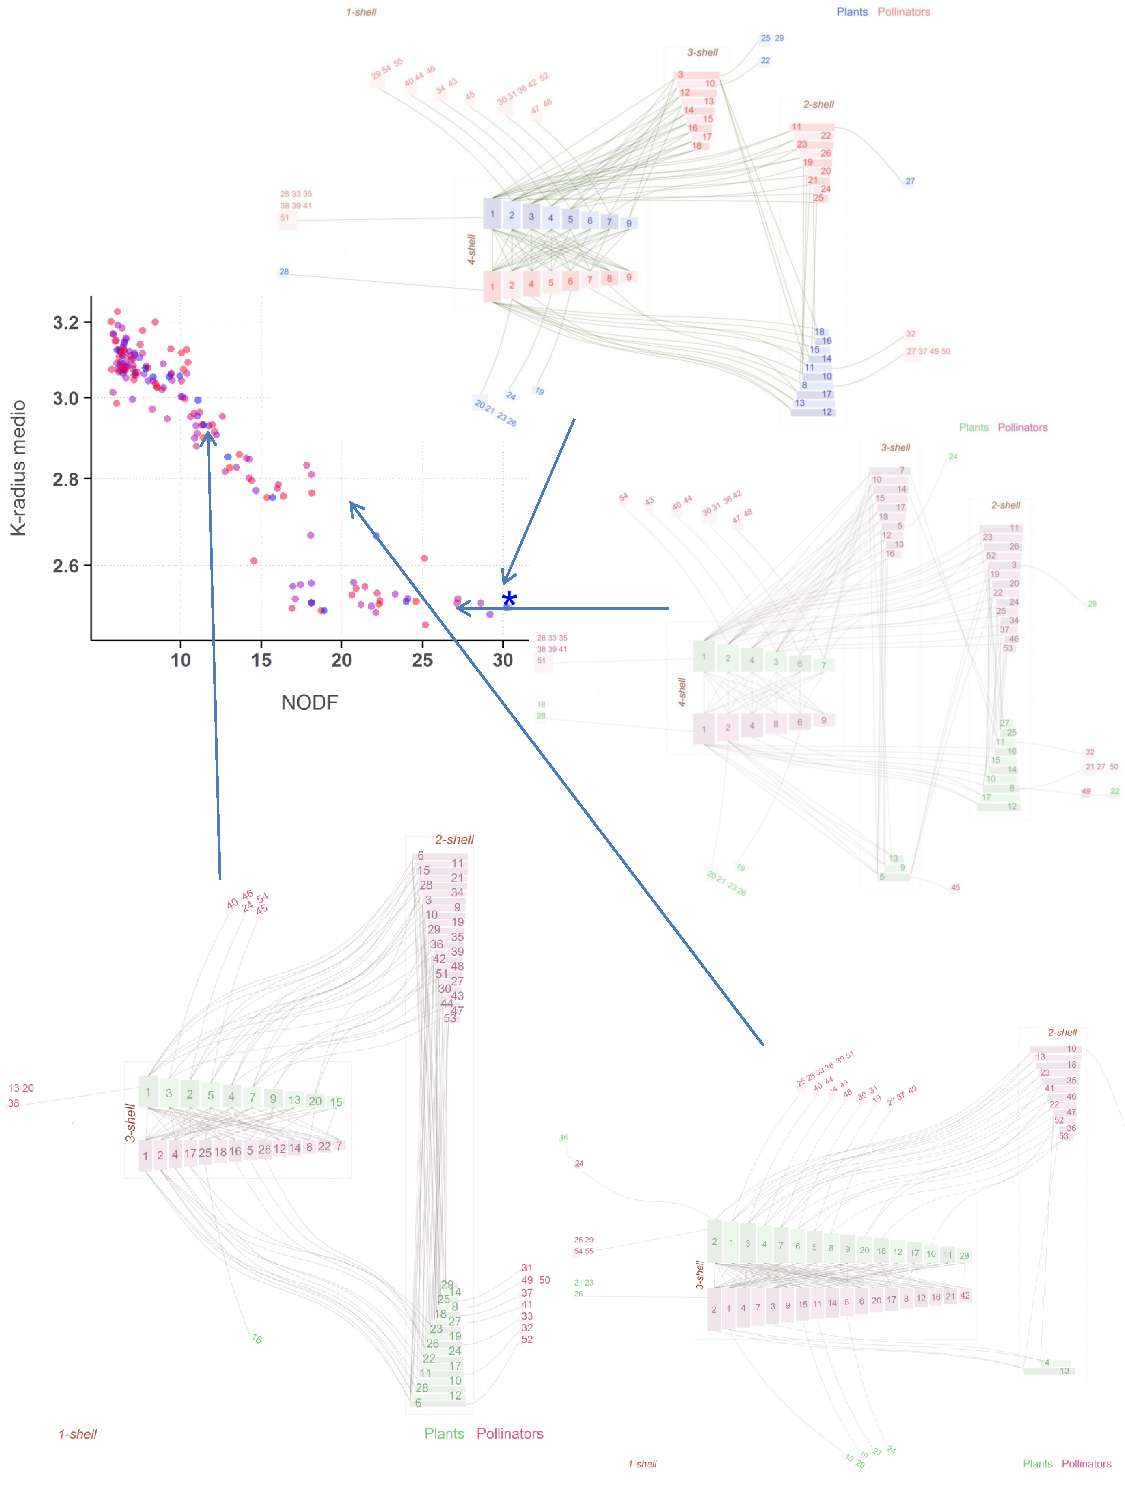
\includegraphics[scale=0.80]{Figures/VIS_PL_012.pdf}
\caption {Red de polinizadores $M\_PL\_012$, en el Parque Nacional de Garajonay, La Gomera (España), compilada por Olesen y no publicada, con $84$ especies y $145$ enlaces. Arriba, la red original, $NODF = 30,40$, $\overline k_{radius} = 2,51$. En sentido horario, red con siete enlaces recableados al azar, $NODF = 26,62$, $\overline k_{radius} = 2,48$; con diecisiete enlaces recableados, $NODF = 22,62$, $\overline k_{radius} = 2,77$ y con treinta y dos, $NODF = 13,22$, $\overline k_{radius} = 2,82$.}
\label{fig:VIS_PL_012}
\end{figure}

\clearpage
\begin{figure}[ht!]
\centering
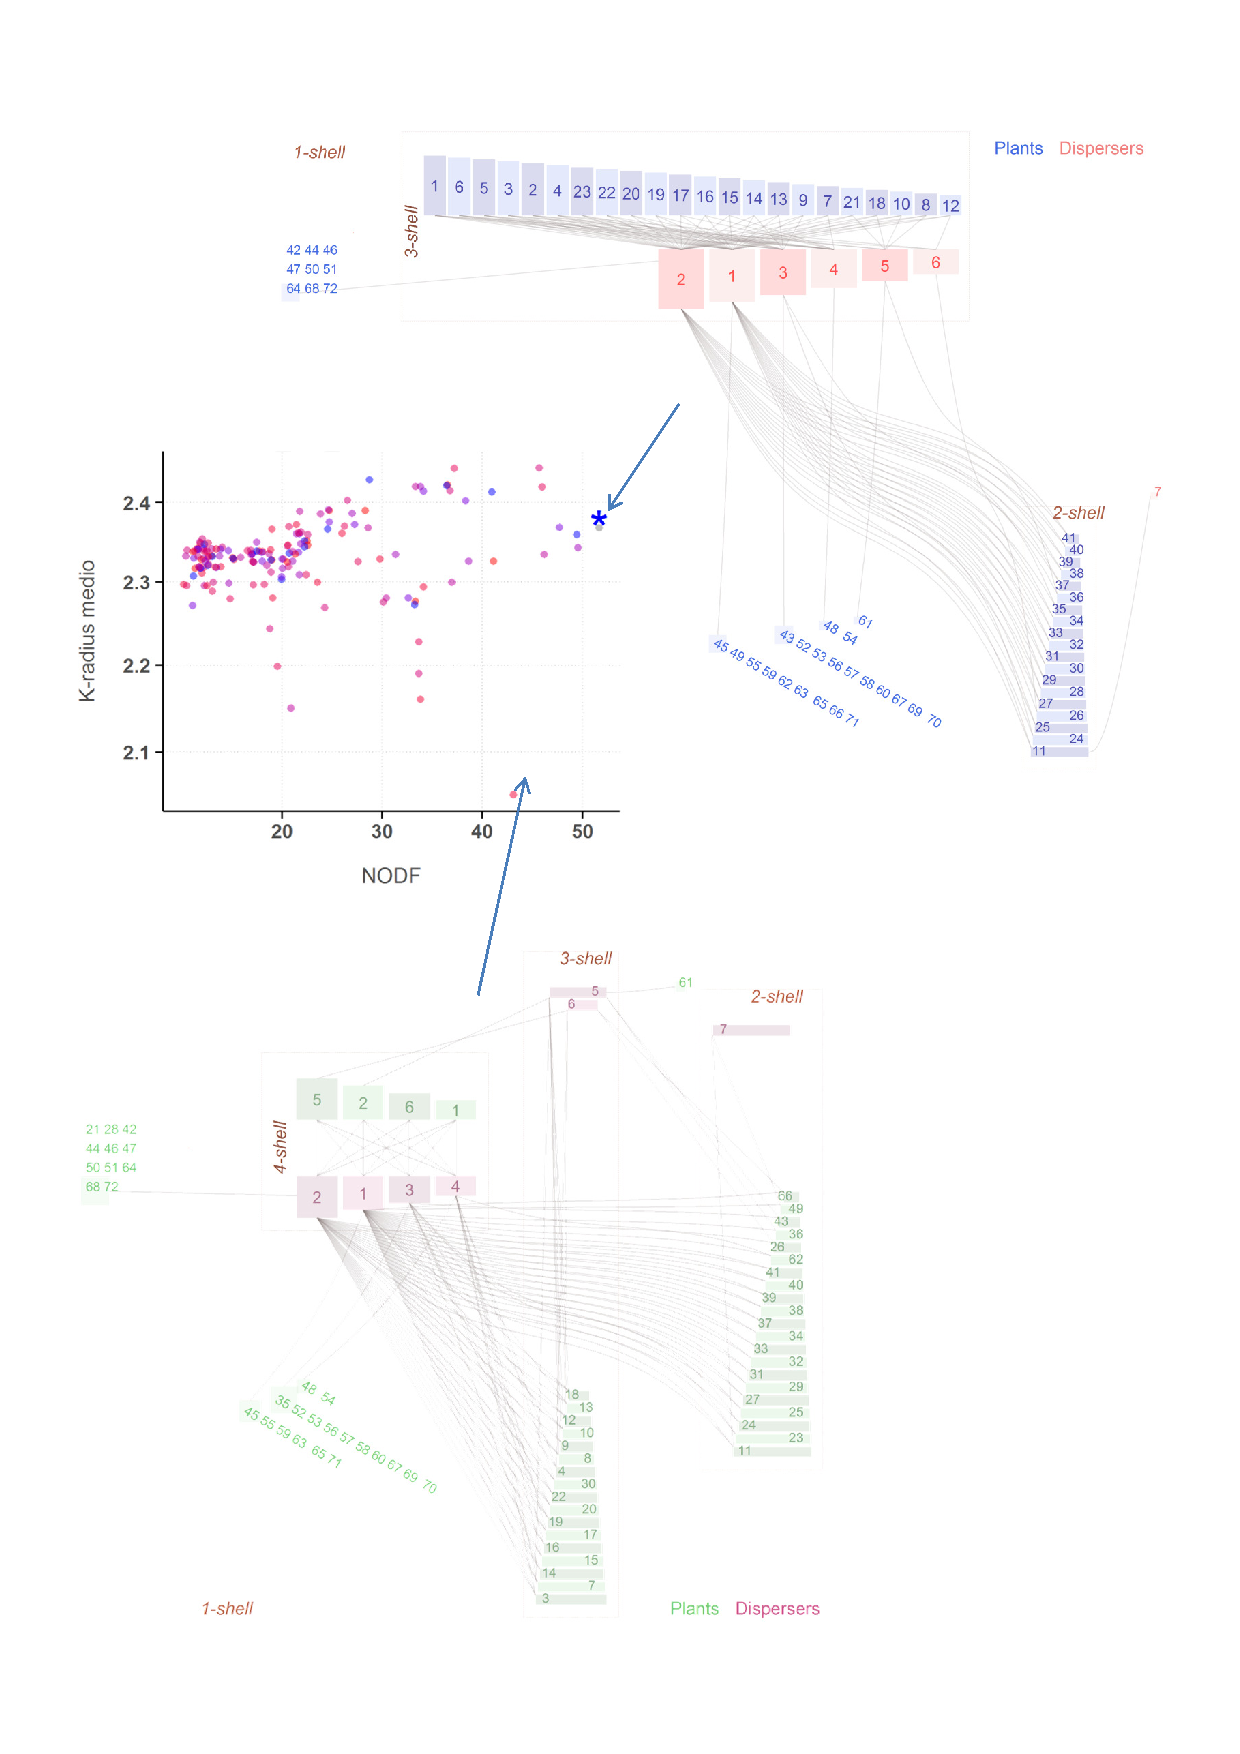
\includegraphics[scale=0.8]{Figures/VIS_SD_007.pdf}
\caption {Red de frugívoros $M\_SD\_007$, en el norte de Queensland, Australia \cite{crome1975ecology}, con $79$ especies y $143$ enlaces. Arriba, la red original, $NODF = 51,67$, $\overline k_{radius} = 2,37$. Abajo, red con seis enlaces recableados al azar, $NODF = 44,75$, $\overline k_{radius} = 2,09$. En el centro el comportamiento de los índices reducidos ante el proceso de recableado.}
\label{fig:VIS_SD_007}
\end{figure}

\clearpage
Con esta configuración parece claro que una alteración mínima de las conexiones de las plantas tendrá un impacto sensible en la estructura global. Es lo que sucede recableando al azar solo seis enlaces. Aparece una $4$-$shell$ y disminuyen a la vez $NODF$ y  $\overline k_{radius}$. En el diagrama de correlación de los índices reducidos se ve que cualquier cambio disminuye el primer parámetro, pero esa información no basta para intuir los profundos cambios de estructura que se desencadenan.

Una situación real en la que las redes cambian de forma drástica se produce por la extinción de una o más especies. En la figura \ref{fig:VIS_M_SD_004_pol3_pol4_ziggurat} se representa la red $M\_SD\_004$ (figura \ref{fig:ziggurat}), en la que se han eliminado únicamente los dos polinizadores de mayor $k_{degree}$, los números $3$ y $4$. El resultado es la reducción en $1$ del índice $k$ máximo, $NODF$ baja desde $39,82$ a $22,46$ y $\overline k_{radius}$ pasa de $2,19$ a $2,26$. La degradación de la red se asemeja a la que se ha visto con el experimento de recableado, con la fusión del $k$ máximo con el $k$-$1$ y el crecimiento de la proporción de enlaces entre especies fuera del $k$ máximo resultante. La red resultante adopta la ya conocida forma de campanilla.

\begin{figure}[ht!]
\centering
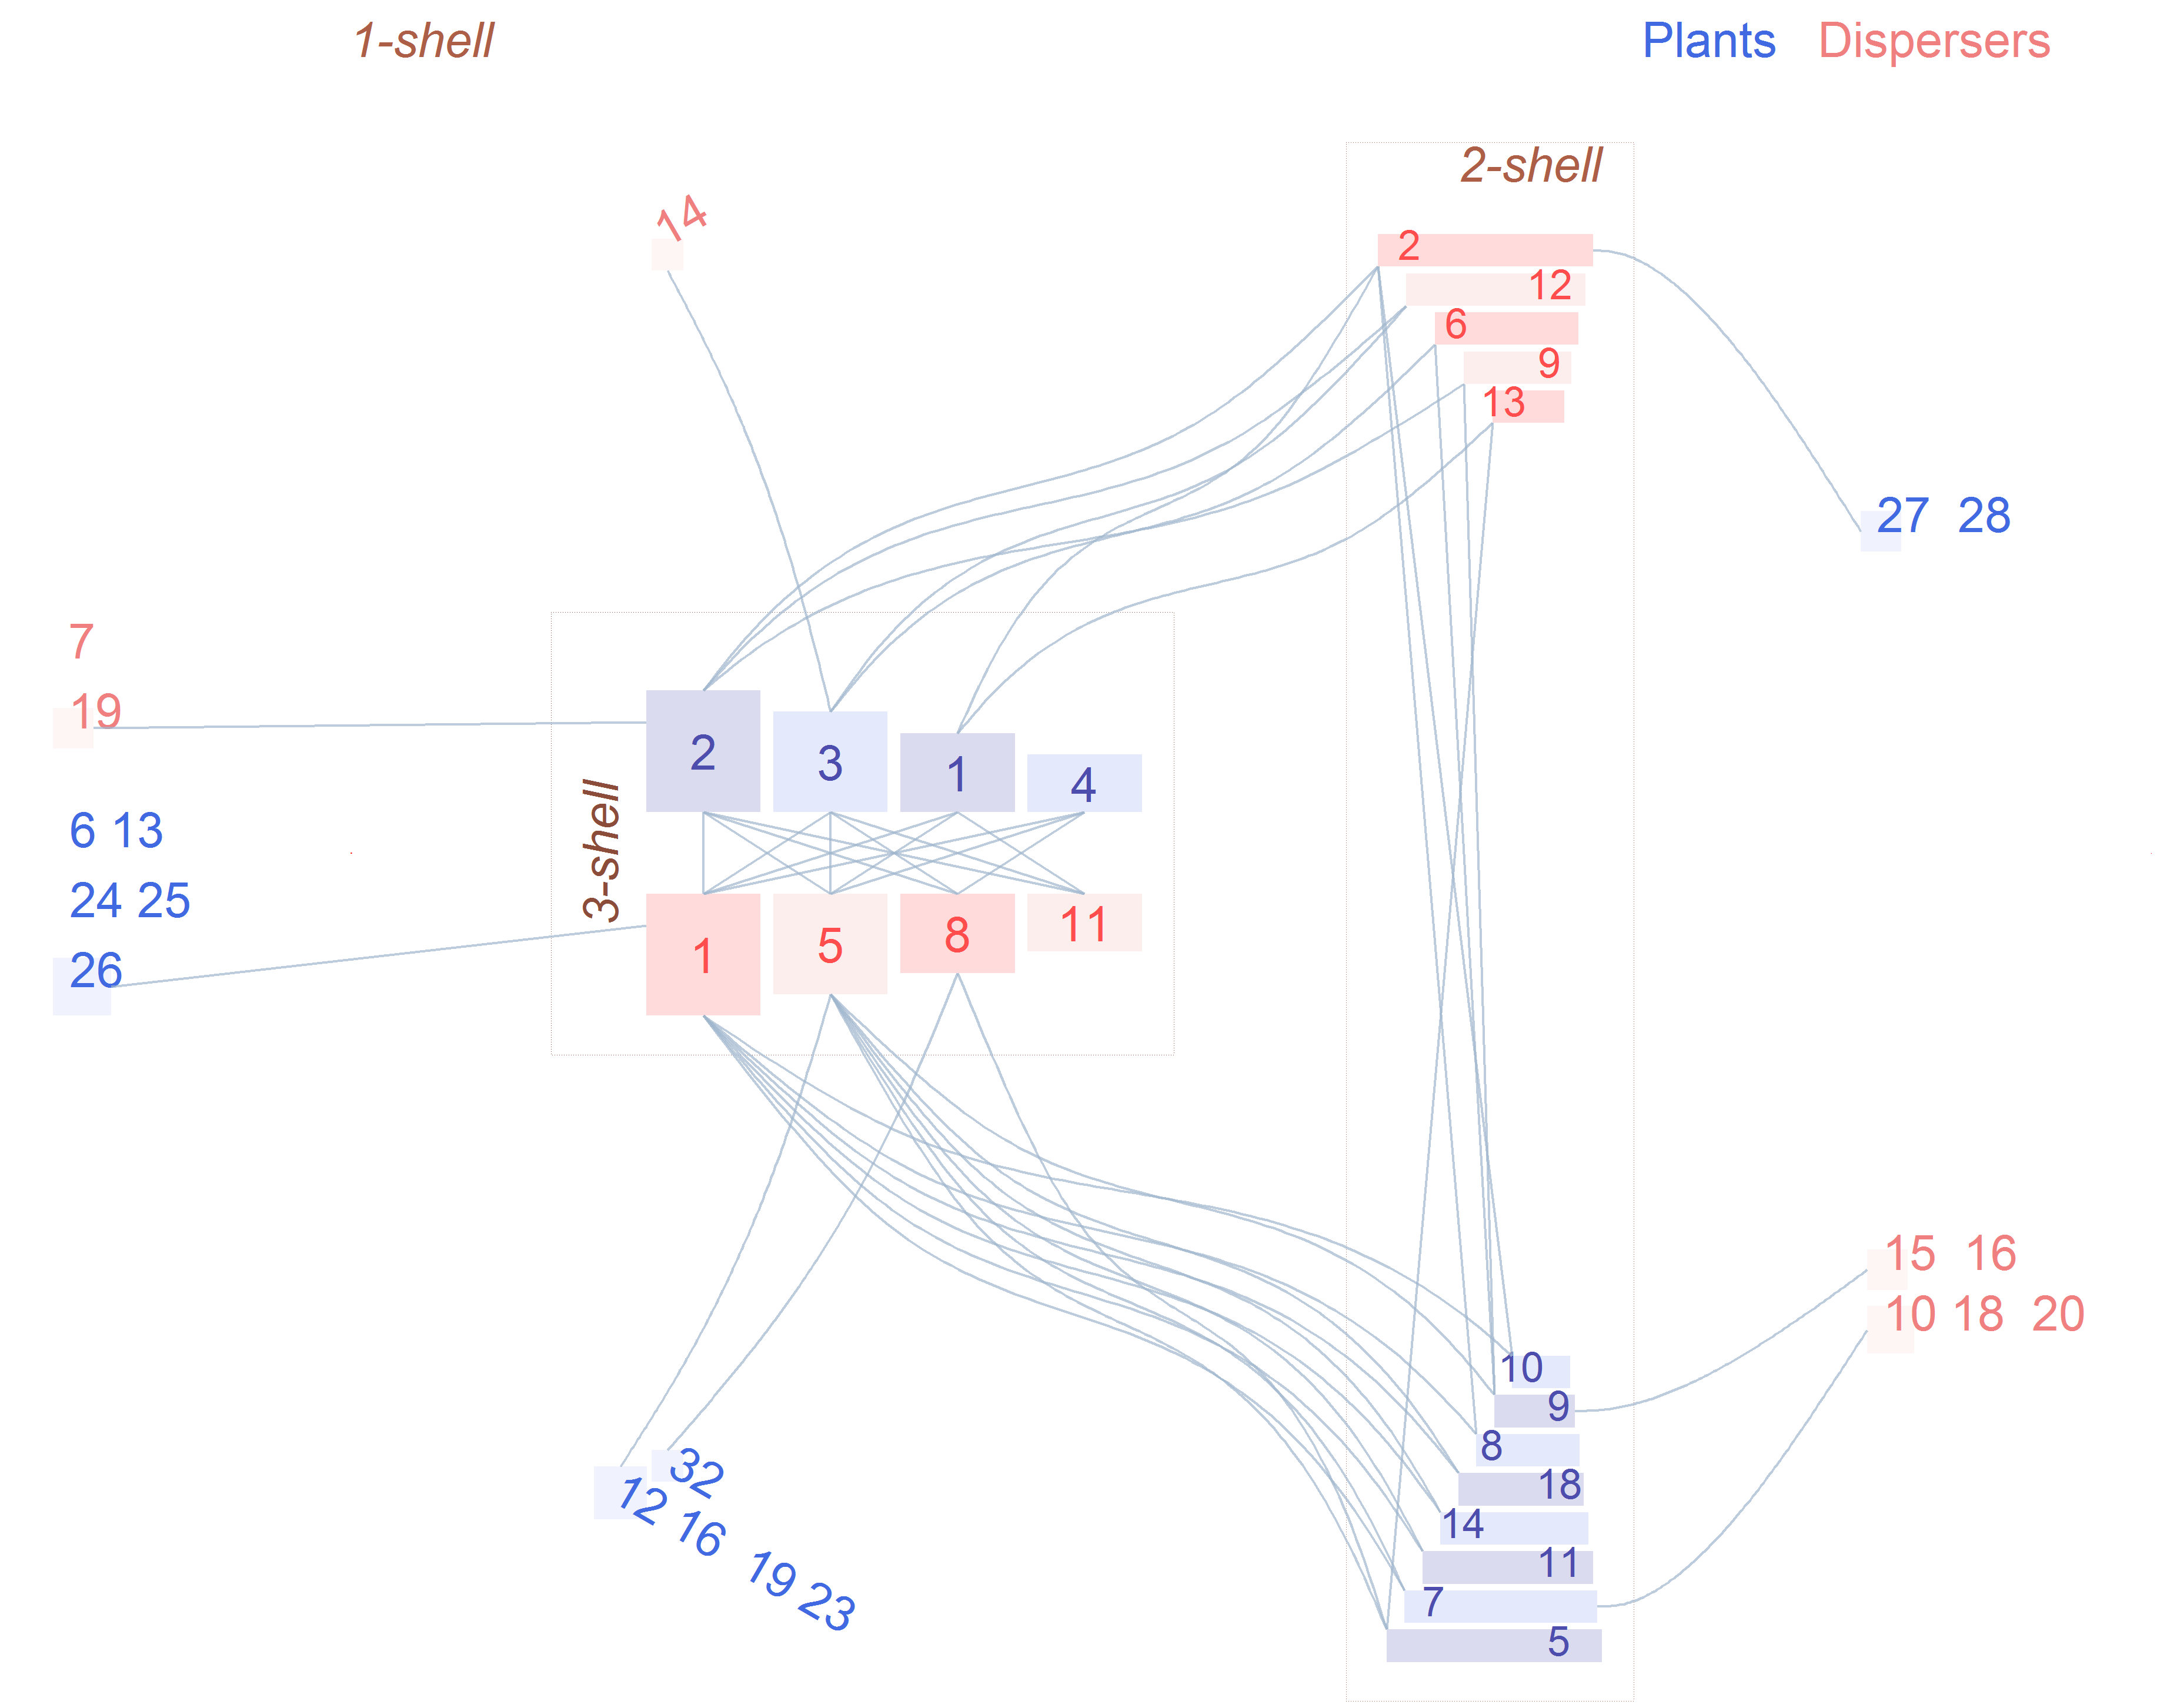
\includegraphics[scale=0.5]{Figures/VIS_M_SD_004_pol3_pol4_ziggurat.png}
\caption {Red de frugívoros $M\_SD\_004$, en la que se han eliminado los polinizadores números $3$ y $4$, los dos de mayor $k_{degree}$, véase la figura \ref{fig:ziggurat}.} 
\label{fig:VIS_M_SD_004_pol3_pol4_ziggurat}
\end{figure}

\clearpage
\begin{figure}[ht!]
\centering
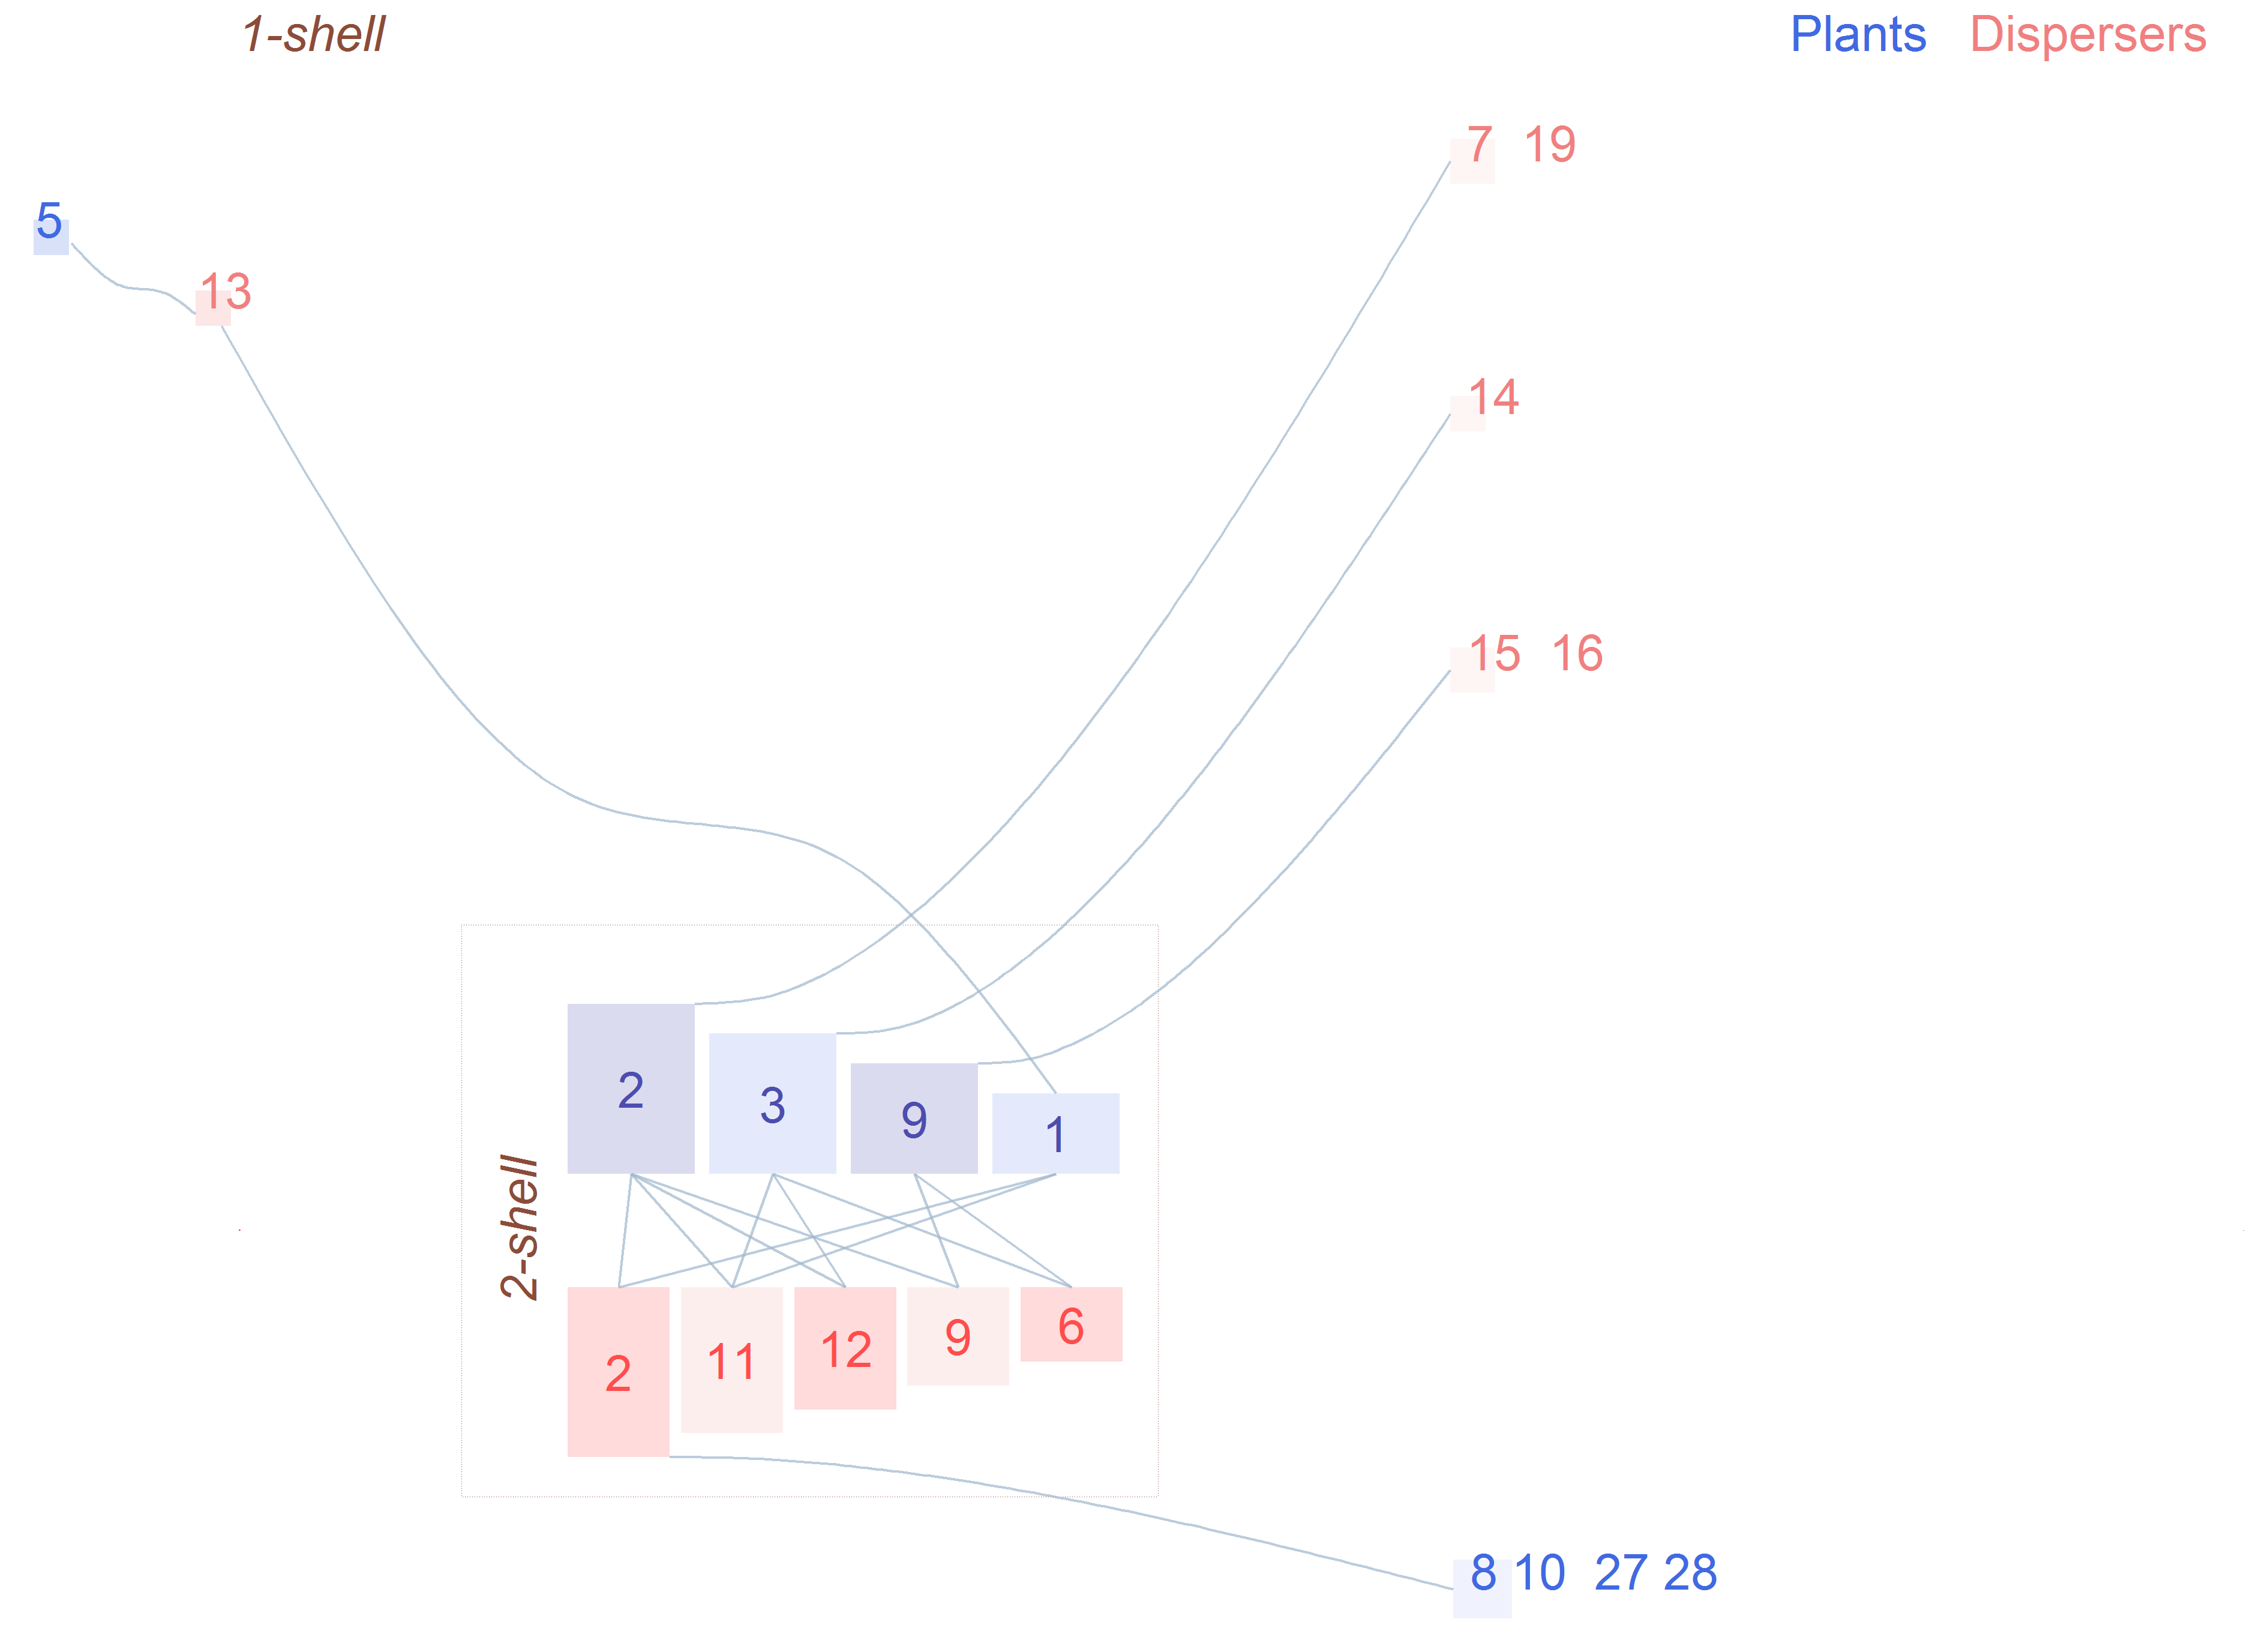
\includegraphics[scale=0.33]{Figures/VIS_M_SD_004_minus_k4_ziggurat.png}
\caption {Red de frugívoros $M\_SD\_004$, en la que se han eliminado todos los polinizadores de la $4$-$shell$, véase la figura \ref{fig:ziggurat}.} 
\label{fig:VIS_M_SD_004_minus_k4_ziggurat}
\end{figure}

\begin{figure}[h!]
\centering
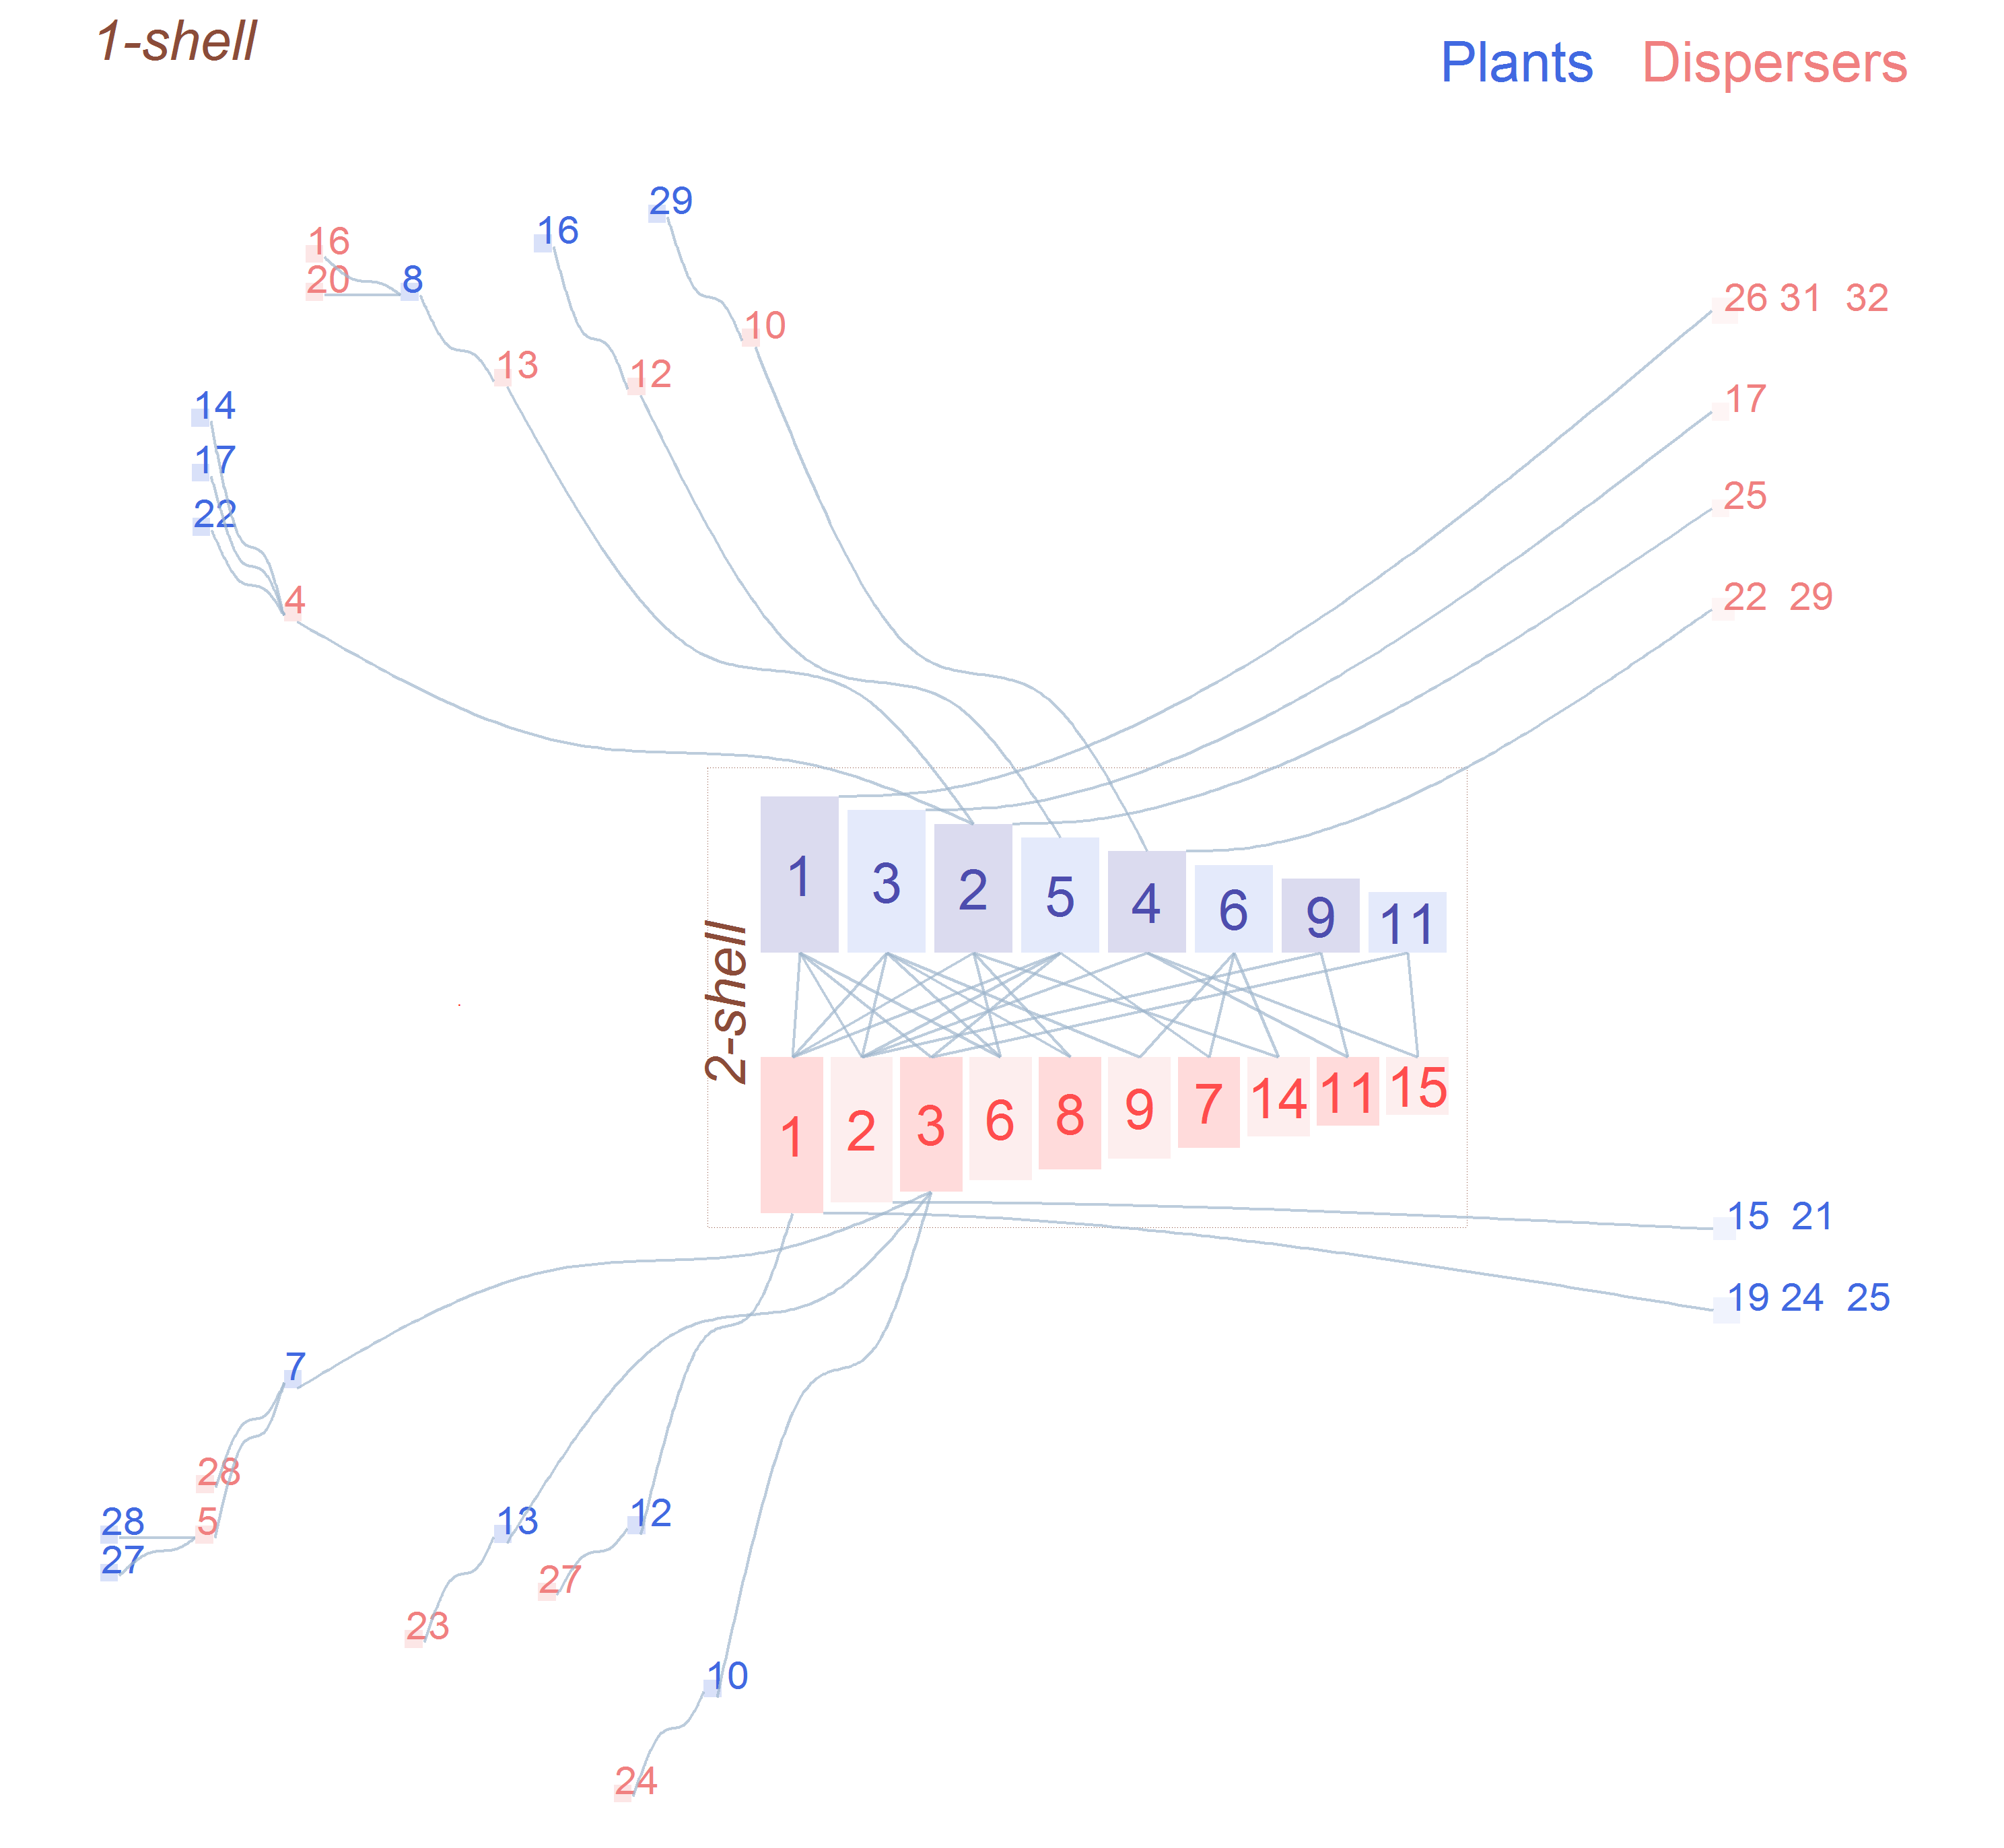
\includegraphics[scale=0.45]{Figures/VIS_M_SD_018_ziggurat.png}
\caption {Red de frugívoros $M\_SD\_018$, en Papúa Nueva Guinea \cite{mack1996notes}.} 
\label{fig:VIS_M_SD_018_ziggurat}
\end{figure}

El diagrama de zigurat permite ver de forma clara la importancia de la \textit{shell} máxima para la estabilidad de la red. Si en la misma red  $M\_SD\_004$ desaparecieran todas las especies de polinizadores de la $4$-$shell$ de manera simultánea ($1$,$3$,$4$,$5$ y $8$) el resultado sería casi catastrófico para la comunidad. El anidamiento cae a $NODF = 3,38$. La red sobreviviente es un pequeño núcleo en $2$-$shell$ y escasas especies en $1$-$shell$ (figura \ref{fig:VIS_M_SD_004_minus_k4_ziggurat}).

En la figura \ref{fig:VIS_Modvskdegree3-sd04} se han representado los diagramas polares de la red intacta, de la red sin los dos polinizadores y de la red sin la $4$-$shell$ y el gráfico de la relación de $\overline k_{degree}$ con $Modularity$ como se hizo en la figura \ref{fig:VIS_Modvskdegree3-sd04}. Desde una posición inicial en la mitad del gráfico, los dos estados degradados se desplazan hacia posiciones de menor $k_{degree}$ y mayor $Modularity$.

\begin{figure}[h!]
\centering
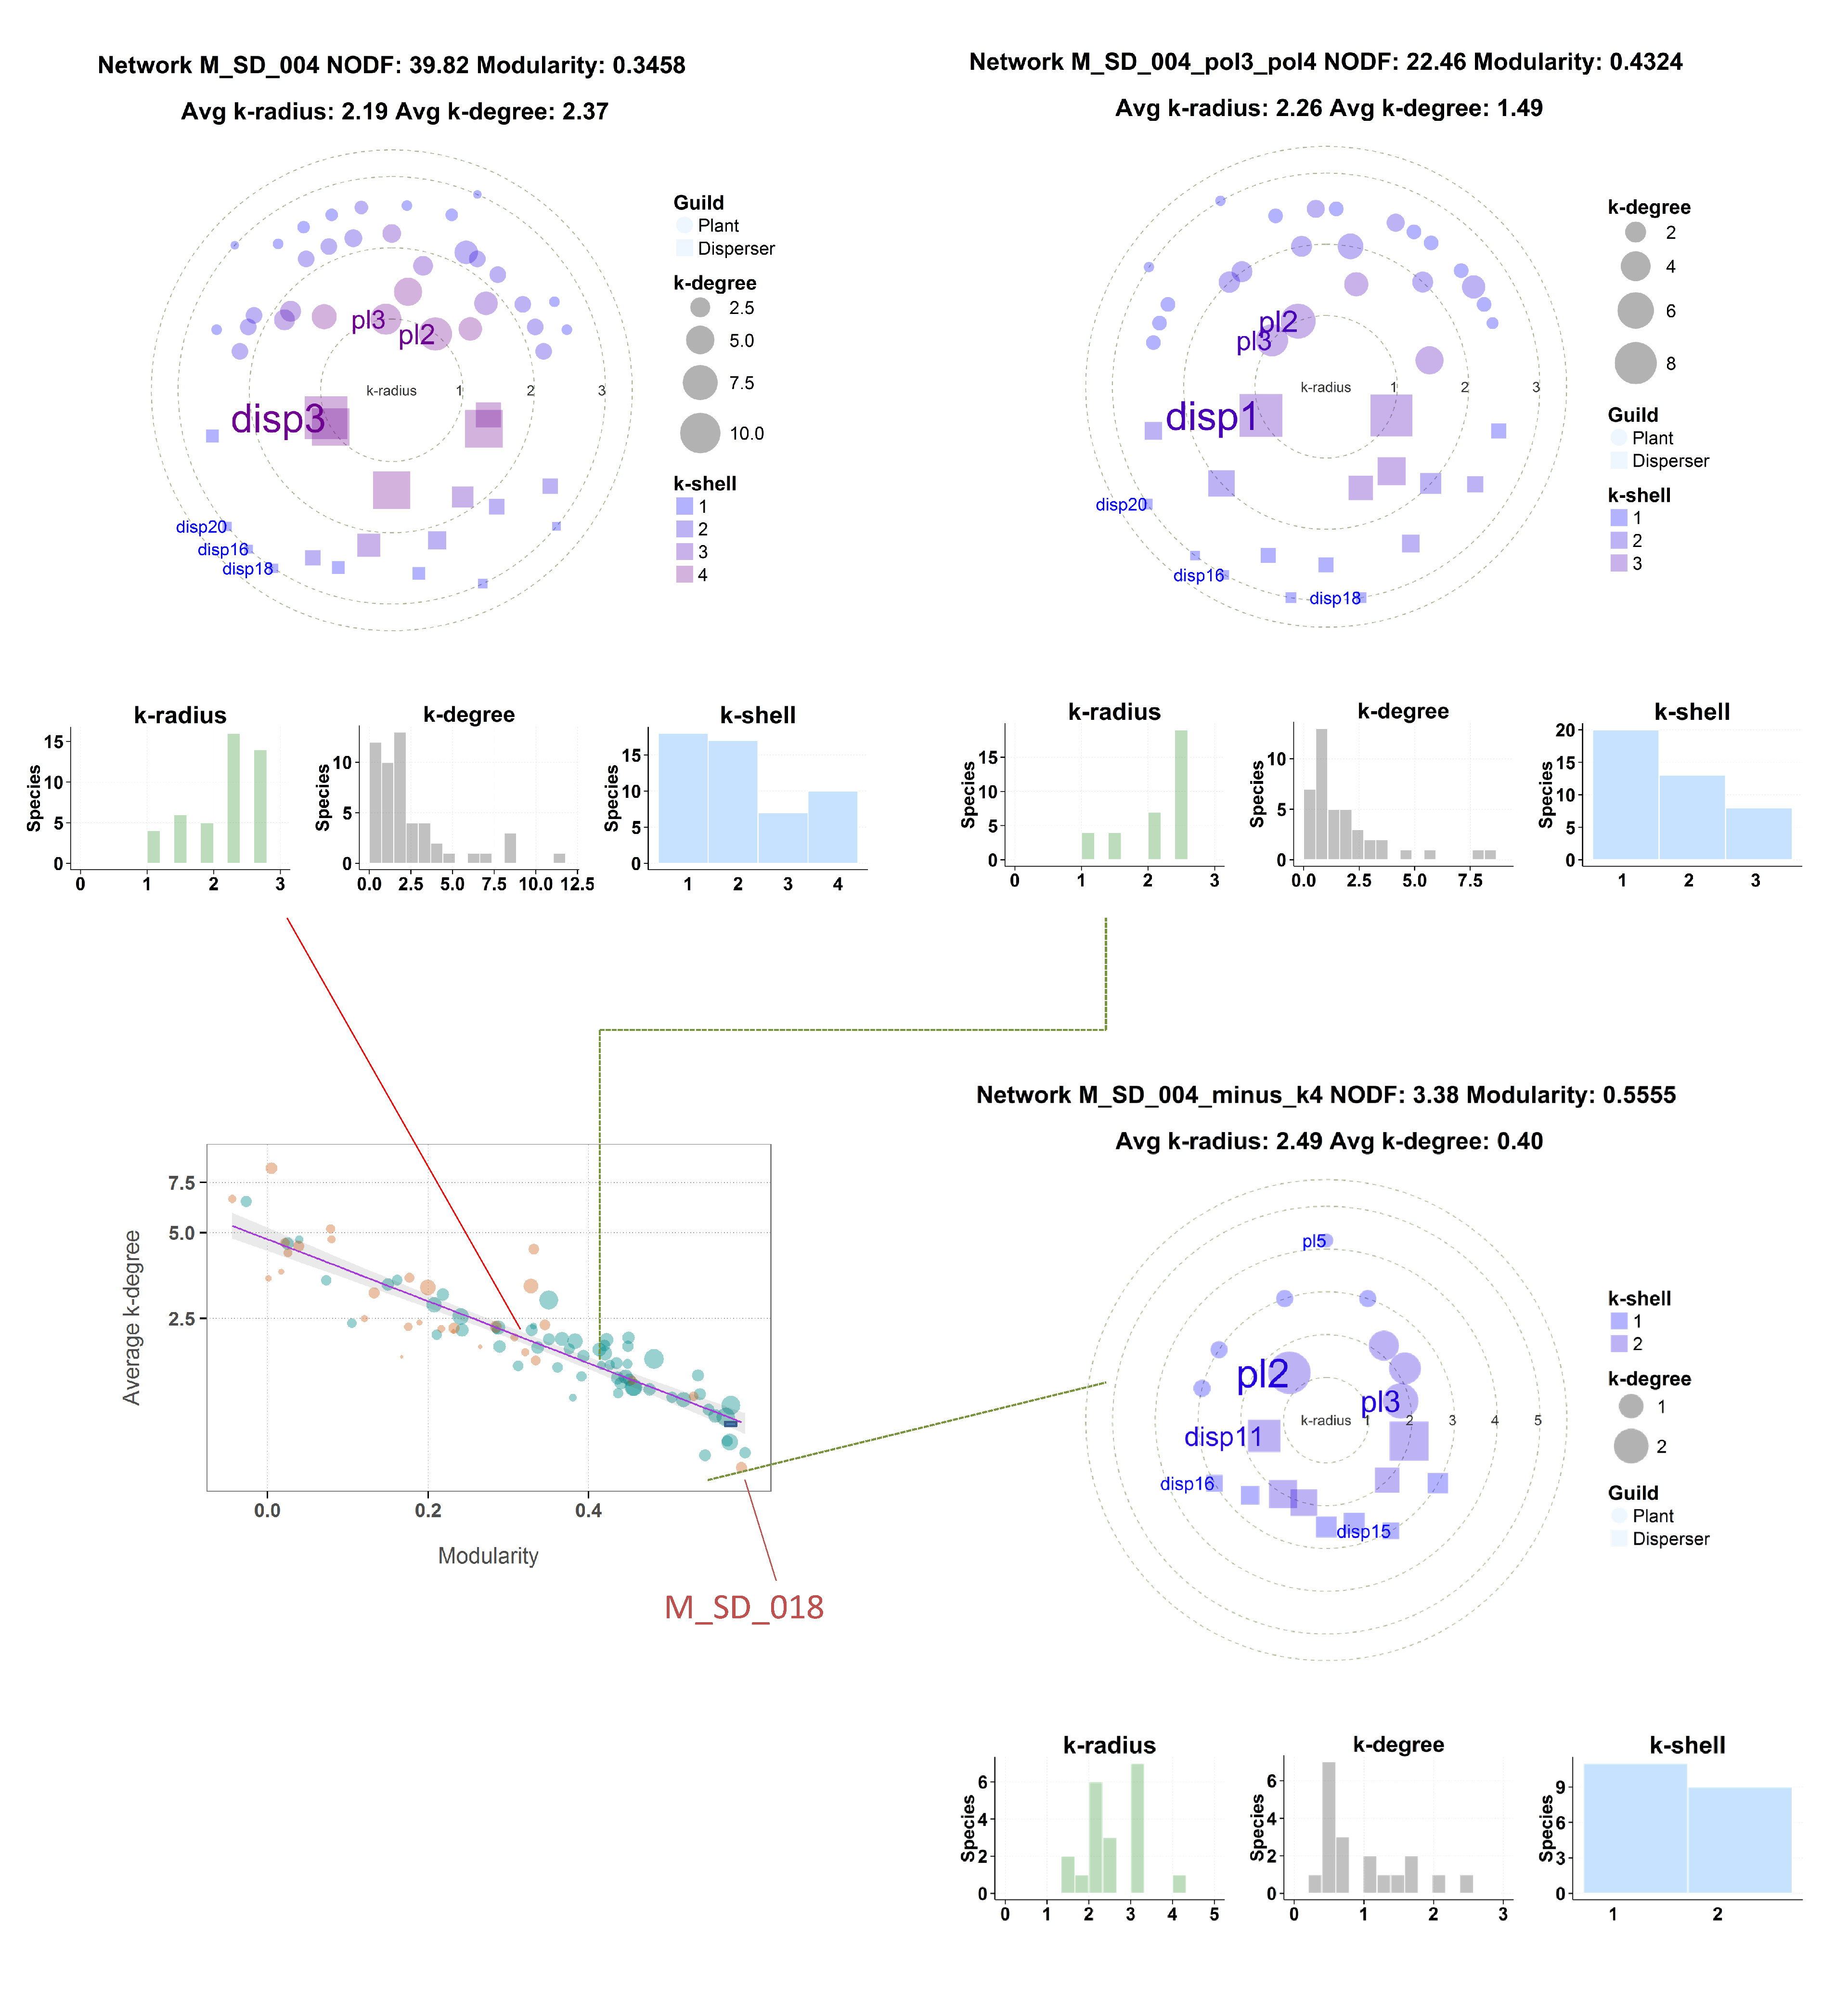
\includegraphics[scale=0.23]{Figures/VIS_Modvskdegree3-sd04.pdf}
\caption {Diagramas polares de la red $M\_SD\_004$ intacta, tras eliminar los dos polinizadores de mayor $k_{degree}$ y tras suprimir la $4$-$shell$ de polinizadores completa.} 
\label{fig:VIS_Modvskdegree3-sd04}
\end{figure}
 
\clearpage
\begin{figure}[ht!]
\centering
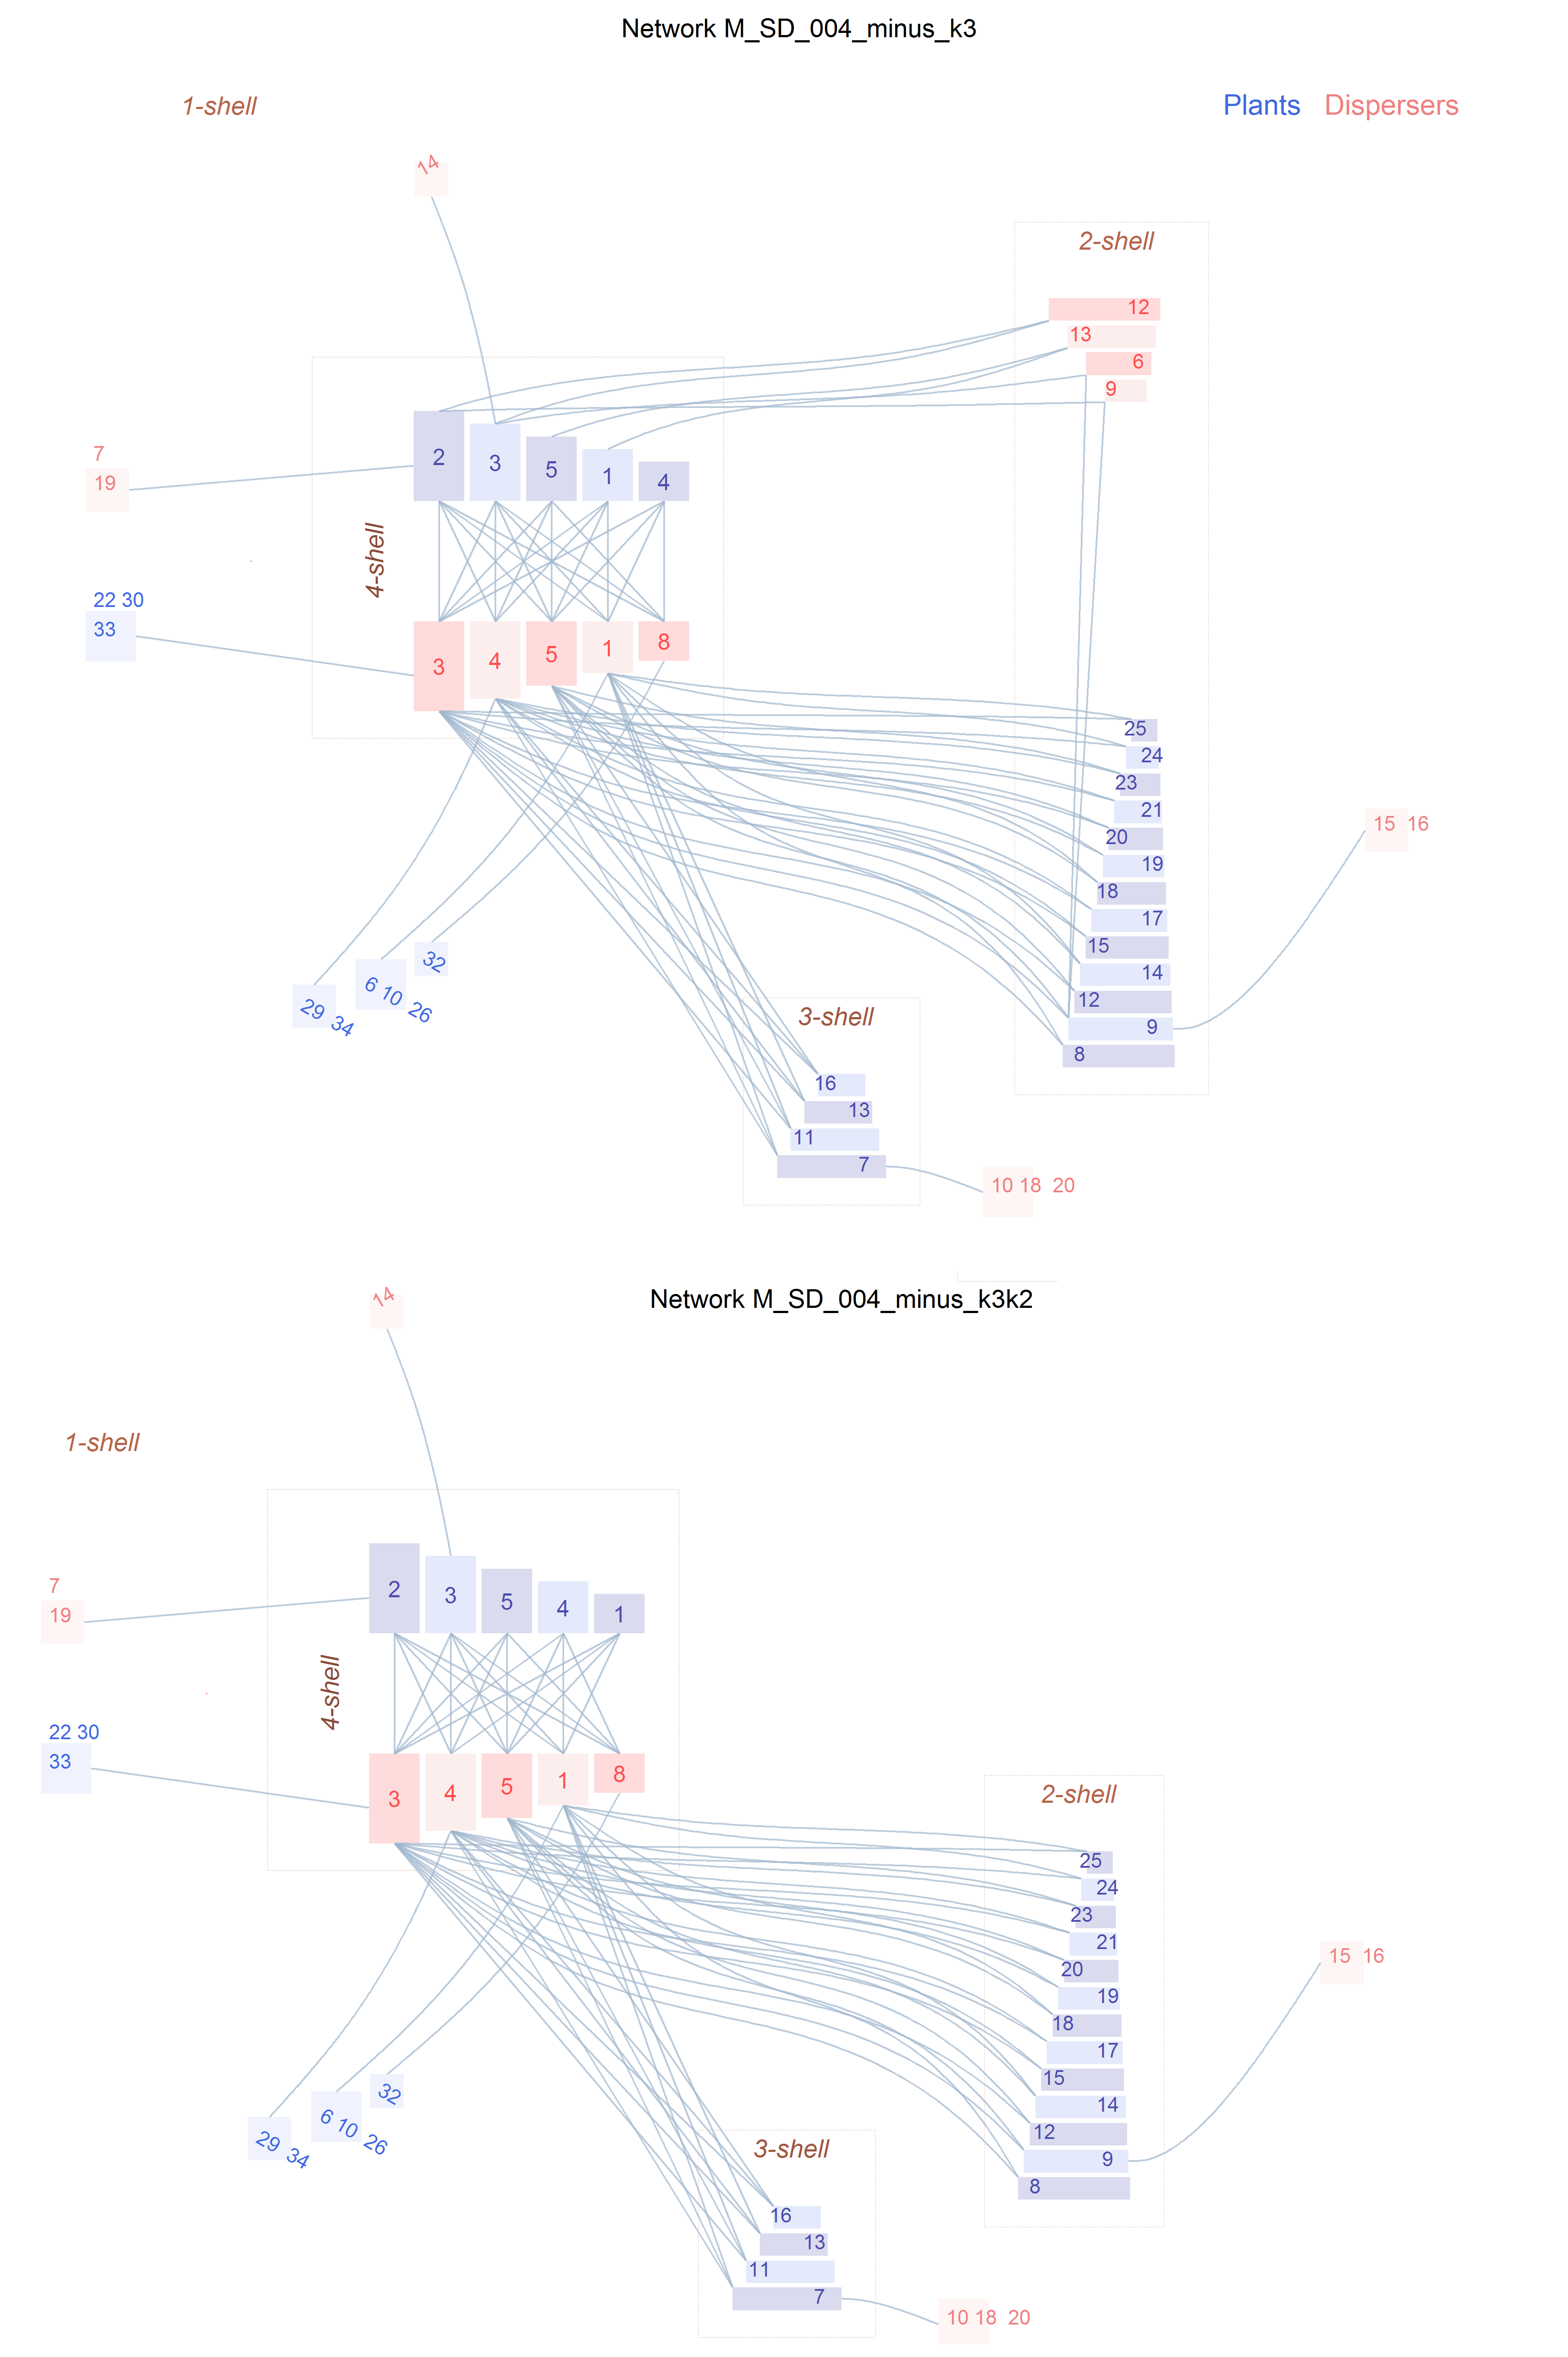
\includegraphics[scale=0.5]{Figures/VIS_M_SD_004_minus_k3k2_ziggurat.png}
\caption {Red de frugívoros $M\_SD\_004$, en la que se han eliminado todos los polinizadores de la $3$-$shell$ ($NODF = 36,24$, $\overline k_{radius} = 2,17$) y la $2$-$shell$ ($NODF = 33,055$, $\overline k_{radius} = 2,15$), véase la figura \ref{fig:ziggurat}.} 
\label{fig:VIS_M_SD_004_minus_k3k2_ziggurat}
\end{figure}

\clearpage
Cabe preguntarse si las redes resultantes de las extinciones se parecen a redes reales. La de toda la colección cuyos parámetros se acercan más a la de la figura \ref{fig:VIS_M_SD_004_minus_k4_ziggurat} es una comunidad de frugívoros que en estado natural tiene un $k$ máximo $2$ (figura \ref{fig:VIS_M_SD_018_ziggurat}). Se ha señalado en el gráfico de correlación de \ref{fig:VIS_Modvskdegree3-sd04} la posición de esta red.

Su aspecto general es muy similar al de lo que queda de la comunidad de Puerto Rico al extinguirse los frugívoros de la \textit{shell} máxima. Esto lleva a pensar que las comunidades mutualistas con bajos índices $k$ máximos pueden ser restos de otras anteriores más complejas que han perdido parte de sus nodos. Alternativamente, podrían ser estados iniciales de formación.

Se ha comprobado como afecta a la red $M\_SD\_004$ la pérdida de los cinco frugívoros de la \textit{shell} máxima, ¿qué ocurre si ese núcleo se mantiene y se destruyen los de índices $k$ menores?

En la imagen superior de la figura \ref{fig:VIS_M_SD_004_minus_k3k2_ziggurat}, se han extinguido las dos especies de frugívoros que formaban la $3$-$shell$. La $NODF$ baja muy poco, de $39,82$ a $36,34$ y el $\overline k_{radius}$ prácticamente no se modifica. El contraste es grande si se compara con el resultado de eliminar los dos frugívoros de mayor $\overline k_{degree}$, tanto en el porcentaje de cambio de las magnitudes como en el de la estructura de la red. Se sigue conservando el índice $k$ máximo $4$.

Si a continuación se extinguen las cuatro especies animales de la $2$-$shell$, tampoco se observan grandes cambios en los parámetros de la red resultante (figura \ref{fig:VIS_M_SD_004_minus_k3k2_ziggurat}, abajo). Esto es así porque los frugívoros desaparecidos tenían casi todos sus enlaces con la $4$-$shell$ de plantas, como consecuencia del anidamiento. Apenas hay arrastre de otras especies (solo las dos plantas de la $1$-$shell$ conectadas a la $3$-$shell$ de animales).

Con este ejemplo se puede entender mejor la importancia del orden de extinción basándose únicamente en el orden de las \textit{k-shells}. Si se conservan las \textit{shells} máximas y la red está bien anidada, la pérdida de otras \textit{shells} de índice inferior no arrastra apenas otras especies. Por el contrario, si hay muchos enlaces entre entre estas \textit{shells} inferiores, el fenómeno puede propagarse dando origen a las extinciones en cascada y la red en conjunto resulta más frágil. En el siguiente capítulo se describe con detalle la influencia de la \textit{k-estructura} en la resistencia de la red.

La conservación de las especies de las \textit{shells} máximas debe ser prioritaria porque de ellas depende en gran medida la supervivencia de toda la comunidad, y el diagrama zigurat es una ayuda gráfica para la comprensión de este hecho.

%\section{Conclusiones}
%
%La visualización de datos es una gran ayuda para la investigación, porque permite observar detalles estructurales. Para ello, las herramientas gráficas deben estar adaptadas a las propiedades de la información. Los gráficos más usados en el estudio de las comunidades mutualistas se vuelven muy confusos cuando la red tiene unas pocas decenas de especies. 
%
%La descomposición \textit{k core} ha permitido definir dos nuevos diagramas, denominados polar y zigurat. El diagrama polar utiliza la descomposición
%como mecanismo de reducción de la información. Permite percibir en qué grado la red es jerárquica y es útil para comparar redes con independencia de sus tamaños.
%
%El diagrama zigurat es más rico. Se representan todas las especies y enlaces y revela con claridad la estructura de \textit{k shells}. Tiene aplicación para comparar la evolución temporal de una red, ya sea por extinciones parciales, por experimentos de reconfiguración o por cualquier otra circunstancia que altere el número de especies y su conectividad. Los diagramas de zigurat tienden a adoptar una serie de figuras tipo que permiten deducir a simple vista algunas propiedades de la red.

\clearpage
\section{Anexo: Red del Parque Nacional de Canaima}
\label{ESTATICA_ANEXO_Canaima}
% Table generated by Excel2LaTeX from sheet 'pl31_indiv'
\begin{table}[htbp]
\fontsize{3mm}{3mm}\selectfont
  \centering

    \begin{tabular}{lrrrlrr}
    \toprule
    $Especie$ & $k_{radius}$ & $k_{degree}$ &      & $Especie$ & $k_{radius}$ & $k_{degree}$ \\
    \midrule
    Planta1 & 2,20 & 5,00 &      & Polinizador1 & 1,00 & 9,80 \\
    Planta2 & 1,00 & 5,96 &      & Polinizador2 & 2,33 & 6,37 \\
    Planta3 & 1,00 & 5,53 &      & Polinizador3 & 1,00 & 7,21 \\
    Planta4 & 3,80 & 1,93 &      & Polinizador4 & 1,00 & 6,75 \\
    Planta5 & 1,00 & 5,53 &      & Polinizador5 & 3,00 & 2,80 \\
    Planta6 & 4,20 & 1,67 &      & Polinizador6 & 1,67 & 5,39 \\
    Planta7 & 2,60 & 3,00 &      & Polinizador7 & 3,00 & 1,81 \\
    Planta8 & 1,00 & 5,46 &      & Polinizador8 & 1,00 & 5,43 \\
    Planta9 & 3,00 & 1,79 &      & Polinizador9 & 2,00 & 3,72 \\
    Planta10 & 1,80 & 3,36 &      & Polinizador10 & 3,00 & 1,55 \\
    Planta11 & 1,40 & 4,00 &      & Polinizador11 & 3,00 & 1,58 \\
    Planta12 & 4,20 & 1,20 &      & Polinizador12 & 4,33 & 1,07 \\
    Planta13 & 1,40 & 4,00 &      & Polinizador13 & 3,00 & 1,41 \\
    Planta14 & 2,60 & 2,10 &      & Polinizador14 & 5,00 & 0,65 \\
    Planta15 & 2,60 & 2,10 &      & Polinizador15 & 3,00 & 1,17 \\
    Planta16 & 4,20 & 0,87 &      & Polinizador16 & 3,00 & 0,96 \\
    Planta17 & 2,20 & 2,03 &      & Polinizador17 & 3,00 & 0,84 \\
    Planta18 & 2,60 & 1,76 &      & Polinizador18 & 3,00 & 1,01 \\
    Planta19 & 4,20 & 0,76 &      & Polinizador19 & 3,00 & 1,08 \\
    Planta20 & 2,60 & 1,67 &      & Polinizador20 & 3,00 & 1,10 \\
    Planta21 & 4,60 & 0,73 &      & Polinizador21 & 5,00 & 0,48 \\
    Planta22 & 2,60 & 1,93 &      & Polinizador22 & 5,00 & 0,40 \\
    Planta23 & 2,60 & 1,33 &      & Polinizador23 & 2,33 & 2,00 \\
    Planta24 & 3,40 & 0,56 &      & Polinizador24 & 5,00 & 0,50 \\
    Planta25 & 6,20 & 0,34 &      & Polinizador25 & 2,33 & 2,00 \\
    Planta26 & 4,20 & 0,67 &      & Polinizador26 & 3,00 & 0,72 \\
    Planta27 & 3,40 & 0,67 &      & Polinizador27 & *    & * \\
    Planta28 & 3,40 & 0,53 &      & Polinizador28 & *    & * \\
    Planta29 & 2,60 & 1,43 &      & Polinizador29 & 5,00 & 0,24 \\
    Planta30 & 2,60 & 0,87 &      & Polinizador30 & 5,00 & 0,22 \\
    Planta31 & 3,00 & 0,76 &      & Polinizador31 & *    & * \\
    Planta32 & *    & *    &      & Polinizador32 & *    & * \\
    Planta33 & 4,60 & 0,53 &      & Polinizador33 & 5,00 & 0,24 \\
    Planta34 & 2,60 & 1,33 &      & Polinizador34 & 3,00 & 0,38 \\
    Planta35 & *    & *    &      & Polinizador35 & 4,33 & 0,33 \\
    Planta36 & 4,60 & 0,53 &      & Polinizador36 & 5,00 & 0,24 \\
    Planta37 & 5,00 & 0,39 &      & Polinizador37 & 4,33 & 0,33 \\
    Planta38 & 2,60 & 1,43 &      & Polinizador38 & 7,00 & 0,16 \\
    Planta39 & 2,60 & 1,43 &      & Polinizador39 & 5,00 & 0,22 \\
    Planta40 & 5,40 & 0,20 &      & Polinizador40 & 5,00 & 0,24 \\
    Planta41 & 2,60 & 1,00 &      & Polinizador41 & 5,00 & 0,24 \\
    Planta42 & 5,80 & 0,20 &      & Polinizador42 & 3,67 & 0,38 \\
    Planta43 & 3,40 & 0,33 &      & Polinizador43 & 3,00 & 0,38 \\
    Planta44 & 4,60 & 0,33 &      & Polinizador44 & 5,00 & 0,24 \\
    Planta45 & 4,60 & 0,33 &      & Polinizador45 & 3,00 & 0,45 \\
    Planta46 & 3,00 & 0,50 &      & Polinizador46 & 3,00 & 0,45 \\
    Planta47 & 2,60 & 1,00 &      & Polinizador47 & 6,33 & 0,20 \\
    Planta48 & 3,40 & 0,33 &      & Polinizador48 & 5,00 & 0,26 \\
         &      &      &      & Polinizador49 & 5,00 & 0,22 \\
    \bottomrule
    \end{tabular}%
    \caption{\label{table:kmag_pl_031} \textit{k magnitudes} de la red  de polinizadores $M\_PL\_031$ del Parque Nacional de Canaima, Venezuela, \cite{ramirez1989biologia}. Valores globales: $\overline k_{radius} = 3,39$; $\overline k_{degree} = 1,57$. Las especies desconectadas de la componente gigante aparecen señaladas con asterisco.}
\end{table}%